\subsection{Model Validations}

All five models have been successfully implemented, while the validation with the figures of the respective publications has only been successful to varying degrees. These five chosen models differ drastically in their ways of modelling photosynthesis and complexity. While it is hard to pinpoint an exact measurement of a model's complexity, a common way is to look at the number of quantities used in the model~\cite{dattnerModelSelectionOrdinary2023}. The highest number of quantities is found in the Saadat2021 model, amassing a total of 292,  which dwarves the much smaller models, Fuente2024 and Matuszynska2016, each with a total of 57 and 73 quantities respectively. The Bellasio2019 and Li2021 models have a total of 134 and 96 quantities each, making them both medium-sized models, in respect to the models analyzed here.

\begin{longtable}{lcccccc}
\caption[Summary of Meta-Information of All the Models.]{\textbf{Summary of Meta-Information of All the Models.}\\The number of variables, parameters, reactions, and derived variables and parameters, and total sum are shown for each model. These values have been extracted directly from the model implementations. A derived quantity, is a quantity that is calculated inside the model. The separation between derived variable and parameter is based on expertise and is not based on a strict rule. However, a main aspect that was considered was with what quantity it was derived from. If the quantity was derived from even a single time-dependent quantity, it is considered a derived variable. The model used are Bellasio2019~\cite{bellasioGeneralisedDynamicModel2019}, Fuente2024~\cite{fuenteMathematicalModelSimulate2024}, Li2021~\cite{liImpactIonFluxes2021}, Matuszynska2016~\cite{matuszynskaMathematicalModelNonphotochemical2016}, and Saadat2021~\cite{saadatComputationalAnalysisAlternative2021}} \label{tab:models-meta} \\
\toprule
 & Variables & Parameters & Reactions & Derived Variables & Derived Parameters & Total \\
\midrule
\endfirsthead
\caption[]{\textbf{Summary of Meta-Information of All the Models.}\\The number of variables, parameters, reactions, and derived variables and parameters, and total sum are shown for each model. These values have been extracted directly from the model implementations. A derived quantity, is a quantity that is calculated inside the model. The separation between derived variable and parameter is based on expertise and is not based on a strict rule. However, a main aspect that was considered was with what quantity it was derived from. If the quantity was derived from even a single time-dependent quantity, it is considered a derived variable. The model used are Bellasio2019~\cite{bellasioGeneralisedDynamicModel2019}, Fuente2024~\cite{fuenteMathematicalModelSimulate2024}, Li2021~\cite{liImpactIonFluxes2021}, Matuszynska2016~\cite{matuszynskaMathematicalModelNonphotochemical2016}, and Saadat2021~\cite{saadatComputationalAnalysisAlternative2021}} \\
\toprule
 & Variables & Parameters & Reactions & Derived Variables & Derived Parameters & Total \\
\midrule
\endhead
\midrule
\multicolumn{7}{r}{Continued on next page} \\
\midrule
\endfoot
\bottomrule
\endlastfoot
Bellasio2019 & 13 & 82 & 17 & 6 & 16 & 134 \\
Fuente2024 & 5 & 31 & 10 & 9 & 2 & 57 \\
Li2021 & 13 & 43 & 20 & 13 & 7 & 96 \\
Matuszynska2016 & 6 & 42 & 8 & 11 & 6 & 73 \\
Saadat2021 & 30 & 167 & 46 & 25 & 24 & 292 \\
\end{longtable}


\emph{Editor's note: In the next sections the figures of the original publications of each model have been recreated. It was tried to complete the recreation process as close as possible to make the comparison as easy as possible. It is important to note, that all figures in this section are own recreations and \textbf{none} have been taken from the original publications. On top of that, these results will only show the differences between the recreations and the original figures and will not present the actual scientific findings of these figures, as that was already done in each publication. It is advised to look at the original publications, as these figures are not included here.}

\subsubsection{Bellasio2019}

All five figures of the publication~\cite{bellasioGeneralisedDynamicModel2019} could be recreated, however each to different degrees. In the recreation of the publication's third figure, all but the d subfigure show a matching recreation of the curves as the publication~\figref{fig:bellasio2019-fig3}. The d subfigure, showing the \gls{gs}, shows a higher value for both the ambient \gls{o2} and low \gls{o2} curves in the lower \gls{ca} range, while at the other end of the spectrum both curves show a much higher similarity to the publication. It has to be noted, that the publication curves of the \gls{ca} scan do not line up on the x-values, a difference that has not been represented in the recreation. This same issue persists in the fourth figure, however its recreation was done successfully~\figref{fig:bellasio2019-fig4}.

\begin{figure}
    \centering
    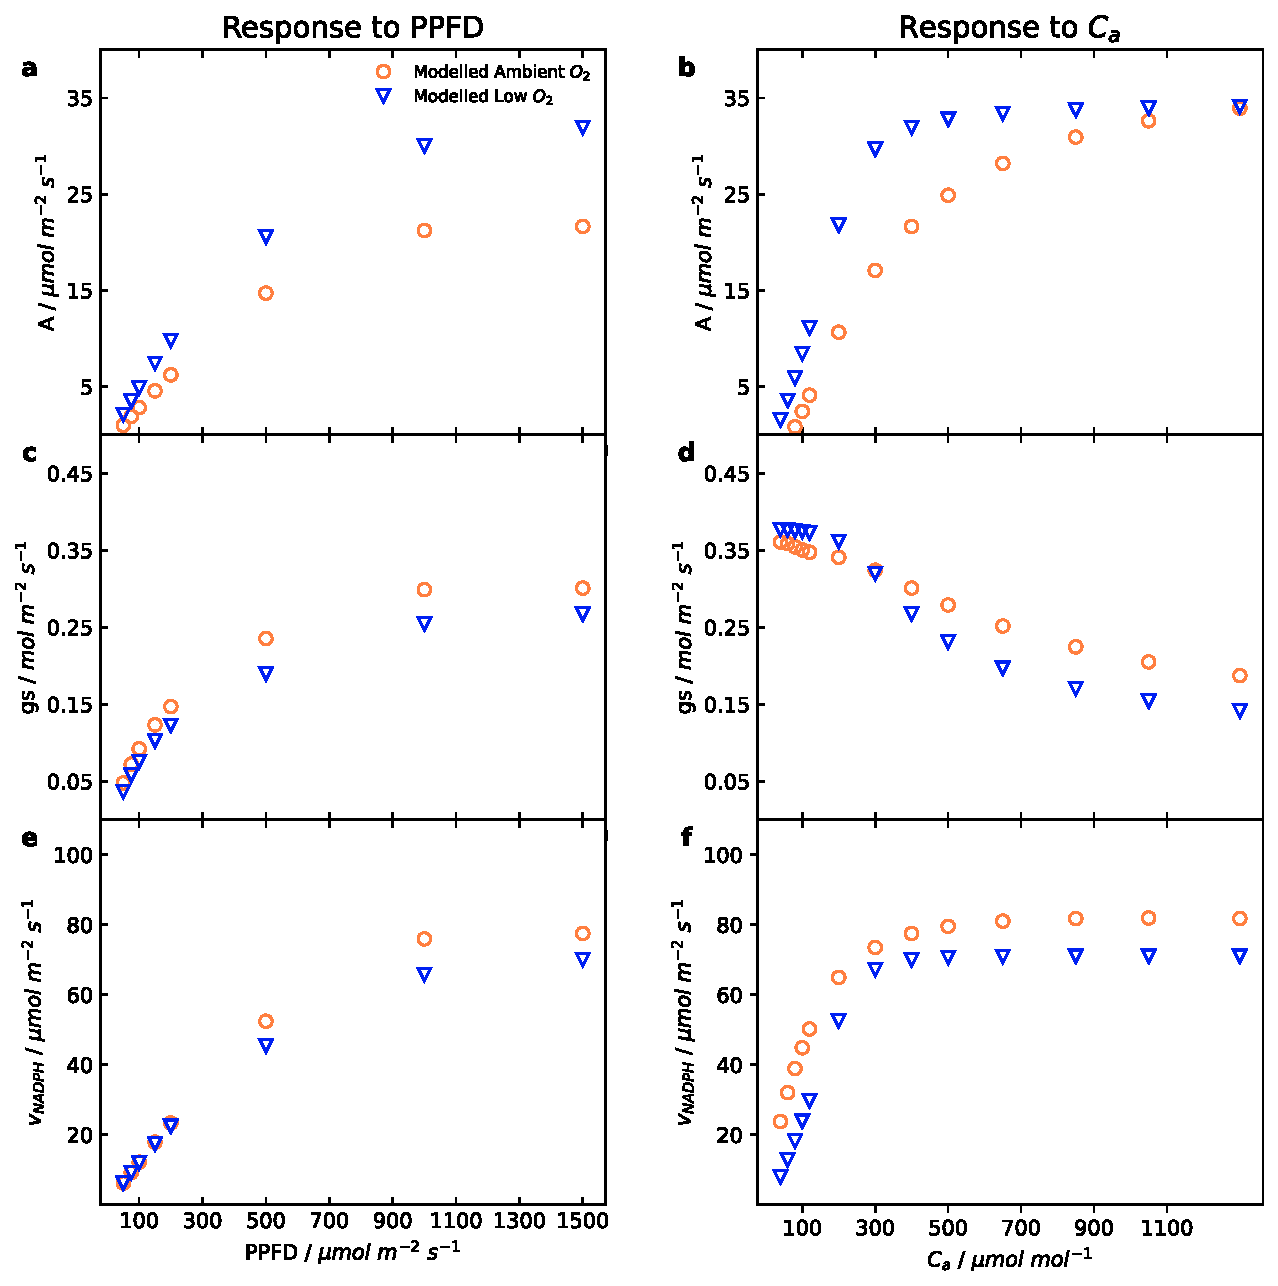
\includegraphics[width=0.7\textwidth]{Figures/Validations/bellasio2019_fig3.pdf}
    \captionvalid{Bellasio2019}{Simulated quasi-steady-state \glsentryshort{ppfd} and \glsentryshort{ca} response curves of different rates.}{A quasi-steady-state scan of \glsentryfull{ppfd} and \glsentryfull{ca} at two different \glsentryfull{o2} concentrations, \qty{210000}{\micro\barp} in orange and \qty{20000}{\micro\barp} in blue. The rates shown, from top to bottom, are \glsentryfull{A}, \glsentryfull{gs}, and \glsentryfull{vfnr}. The scan of \glsentryshort{ppfd} is done at a fixed \glsentryfull{ca} of \qty{400}{\micro\barp}, while the scan of \glsentryshort{ca} is done at a fixed \glsentryshort{ppfd} of \qty{1500}{\micro\mol\per\square\meter\per\second}. The other parameters are kept at their default values. The \glsentryshort{ppfd} values used are 50, 75, 100, 150, 200, 500, 1000, and 1500. For \glsentryshort{ca} are 400, 300, 200, 120, 100, 80, 60, 40, 400, 400, 400, 400, 500, 650, 850, 1050, and 1300. As steady-state cannot be always reached within this model, a quasi-steady-state is assumed to be at a maximum time of \qty{1800}{s}. This figure is recreated from figure 3 of the original publication of the Bellasio2019 model~\cite{bellasioGeneralisedDynamicModel2019}. The experimental data could not be plotted, as there was no access to it. In the publication it is said that a scan of \glsentryfull{ci} was done instead of \glsentryshort{ca}, however, due to many reasons, \glsentryshort{ca} is used here, even though the values of the x-axis are not identical.}
    \label{fig:bellasio2019-fig3}
\end{figure}

\begin{figure}
    \centering
    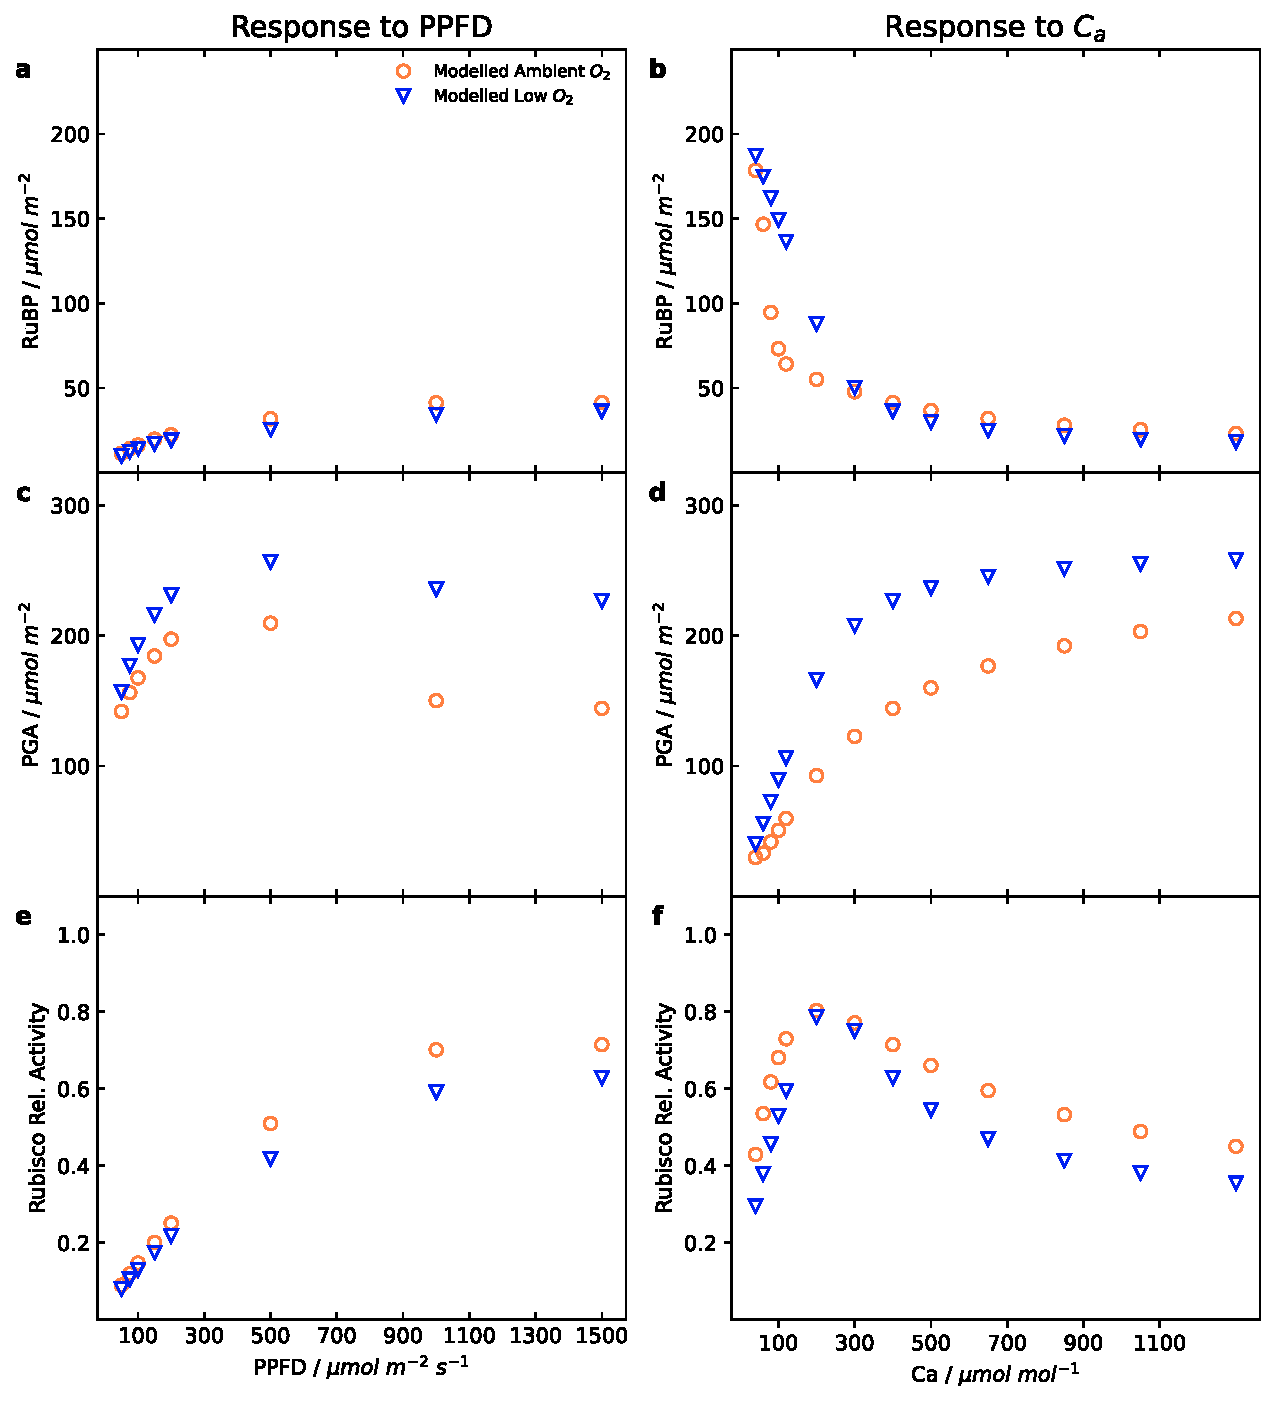
\includegraphics[width=0.7\textwidth]{Figures/Validations/bellasio2019_fig4.pdf}
    \captionvalid{Bellasio2019}{Simulated quasi-steady-state \glsentryshort{ppfd} and \glsentryshort{ca} response curves of metabolic concentrations.}{A quasi-steady-state scan of \glsentryfull{ppfd} and \glsentryfull{ca} at two different \glsentryfull{o2} concentrations, \qty{210000}{\micro\barp} in orange and \qty{20000}{\micro\barp} in blue. The metabolic concentrations shown, from top to bottom, are \glsentryfull{rubp}, \glsentryfull{pga}, and the relative \glsentryfull{rubisco} activity. The two first mentioned were multiplied by the \glsentryfull{Vm} to come to a per area unit and the last is a product of the \glsentryfull{frubp} and the \glsentryfull{Ract}. The scan of \glsentryshort{ppfd} is done at a fixed \glsentryfull{ca} of \qty{400}{\micro\barp}, while the scan of \glsentryshort{ca} is done at a fixed \glsentryshort{ppfd} of \qty{1500}{\micro\mol\per\square\meter\per\second}. The other parameters are kept at their default values. The \glsentryshort{ppfd} values used are 50, 75, 100, 150, 200, 500, 1000, and 1500. For \glsentryshort{ca} are 400, 300, 200, 120, 100, 80, 60, 40, 400, 400, 400, 400, 500, 650, 850, 1050, and 1300. As steady-state cannot be always reached within this model, a quasi-steady-state is assumed to be at a maximum time of \qty{1800}{s}. This figure is recreated from figure 4 of the original publication of the Bellasio2019 model~\cite{bellasioGeneralisedDynamicModel2019}. The experimental data could not be plotted, as there was no access to it. In the publication it is said that a scan of \glsentryfull{ci} was done instead of \glsentryshort{ca}, however, due to many reasons, \glsentryshort{ca} is used here, even though the values of the x-axis are not identical.}
    \label{fig:bellasio2019-fig4}
\end{figure}

The fifth figure has mixed results, when it comes to its recreation~\figref{fig:bellasio2019-fig5}. In all subfigures of the recreation, the first phase of the transition was kept before the zero-point of the x-axis, which is missing in the publication. This was done to make it easier to interpret if the simulation run first also had problems. The results of \gls{A}, \gls{vatp}, \gls{vfnr} at a transition of \qty{50}{\micro\mol\per\square\meter\per\second} to \qty{1500}{\micro\mol\per\square\meter\per\second} match the publication well~\figref[a]{fig:bellasio2019-fig5}, while the reverse transition shows a slightly slower acclimation to the new light intensity~\figref[b]{fig:bellasio2019-fig5}. This same issue persists with the \gls{frubp} in the high to low acclimation~\figref[d]{fig:bellasio2019-fig5}, while the \gls{frubp} in the low to high transition has the same results at the start, but ends at a lower value than the publication~\figref[c]{fig:bellasio2019-fig5}. Both the \gls{Ract} and the \gls{gs} were identically recreated~\figref[c and d]{fig:bellasio2019-fig5}. The results of \gls{pga} end at the identical value to the publication, but the transition is much faster in the low to high light and much slower in the high to low light~\figref[e and f]{fig:bellasio2019-fig5}. The \gls{Pi} results show the same slow acclimation in the low to high transition, however, the recreation recuperates from the fall to a much higher value than the publication~\figref[e]{fig:bellasio2019-fig5}. In the high to low transition, the recreation shows a small negative dip after the transition point and then rises to a stable value, while the publication, has a steady rise to a peak, which falls off a small bit to same stable value as the recreation~\figref[f]{fig:bellasio2019-fig5}. The \gls{rubp} and \gls{dhap} curves in the high to low transition both show a very similar pattern to the publication, except for the same acclimation problem explained prior with \gls{frubp}~\figref[f]{fig:bellasio2019-fig5}. On the low to high transition, however, the \gls{dhap} curve is deemed identical to the publication, while the \gls{rubp} curve shows a faster but with lower peak acclimation than the publication. On top of that, the stable value reached by the \gls{rubp} curve is also lower in the recreation\gls{frubp}~\figref[e]{fig:bellasio2019-fig5}. Lastly, both the ratios of \gls{atp} and \gls{nadph} to their respective totals show a much faster acclimation in the low to high transition, while stabilizing at a higher value than the publication~\figref[g]{fig:bellasio2019-fig5}. The same acclimation issue as with \gls{frubp} is seen in the high to low transition, while the stable value of the \gls{atp} curve is higher and of the \gls{nadph} curve is lower compared to the publication~\figref[h]{fig:bellasio2019-fig5}

\begin{figure}
    \centering
    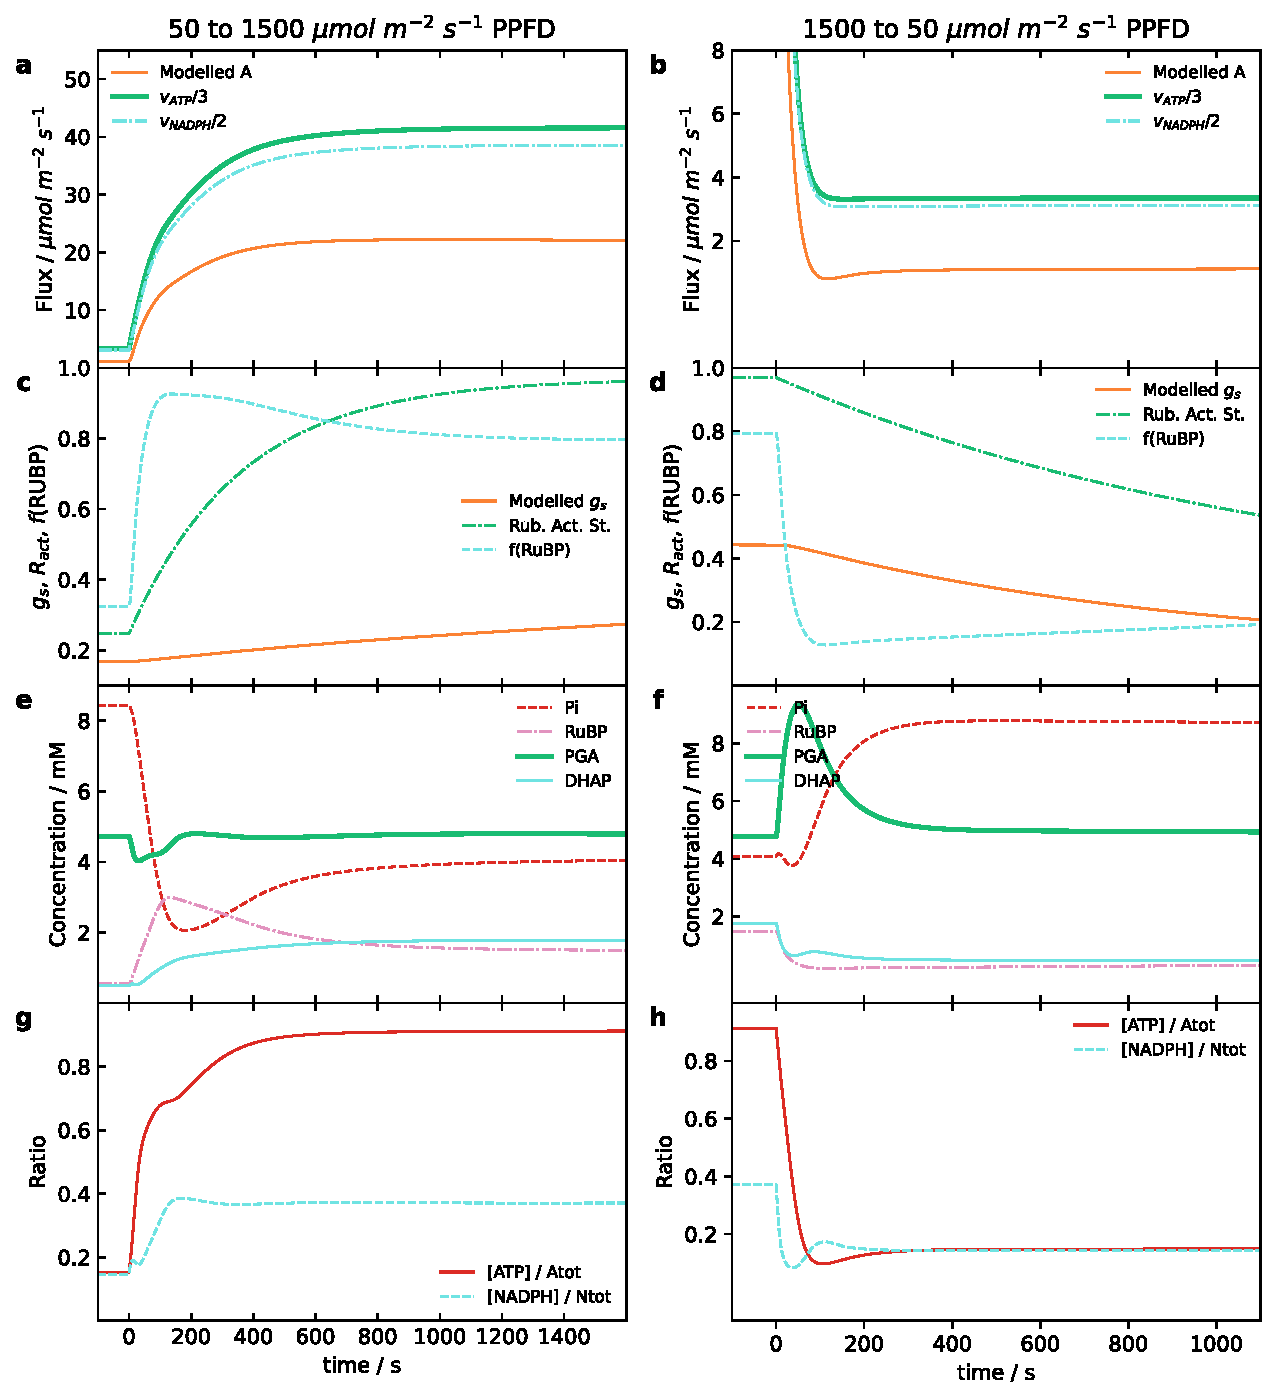
\includegraphics[width=0.7\textwidth]{Figures/Validations/bellasio2019_fig5.pdf}
    \captionvalid{Bellasio2019}{Simulated transition between different \glsentryshort{ppfd}.}{The simulations were done with an acclimation period of \qty{400}{\second} and a second period that reaches quasi-steady-state at \qty{1800}{\second}. Each period is done with a different \glsentryfull{ppfd} to show a transition. On the left, a low to high light intensity, \qty{50}{\micro\mol\per\square\meter\per\second} and \qty{1500}{\micro\mol\per\square\meter\per\second}, transition is done, while on the right the reverse is done. This switch is the zero point on the x-axis. The simulation is run using the default parameters, except \glsentryfull{ca} ($=\qty{350}{\micro\barp}$), \glsentryfull{vcmax} ($=\qty{0.18}{\milli\mol\per\meter\squared\per\second}$), \glsentryfull{tau0} ($=\qty{-0.12}{}$), \glsentryfull{Ki} ($=\qty{3600}{\second}$), and \glsentryfull{Kd} ($=\qty{1200}{\second}$). These parameters were chosen to mimic the environment of the experimental work done. The top row shows the \glsentryfull{A}, the \glsentryfull{vatp}, and \glsentryfull{vfnr}. The top-middle row shows the \glsentryfull{gs}, \glsentryfull{Ract}, and \glsentryfull{frubp}. The bottom-middle row shows the \glsentryfull{Pi}, \glsentryfull{rubp}, \glsentryfull{pga}, and \glsentryfull{dhap}. Lastly, the bottom row shows the ratio of \glsentryfull{atp} and \glsentryfull{nadph} to their respective totals. This figure is recreated from figure 5 of the original publication of the Bellasio2019 model~\cite{bellasioGeneralisedDynamicModel2019}. The experimental data could not be plotted, as there was no access to it.}
    \label{fig:bellasio2019-fig5}
\end{figure}

The sixth figure shows no similarity to the publication at all. However, many transition points, the zero-point on the axis, show a change in the slope of the continuing curves, hinting at a change in the simulation~\figref{fig:bellasio2019-fig6}. The seventh and final figure on the other hand, was successfully recreated, with both the \gls{A} and \gls{phipsii} curves showing the same pattern and values as the publication~\figref{fig:bellasio2019-fig7}. The only difference, is that the \gls{A} at the transition point of ambient to low \gls{o2} is much smoother in the recreation than it is in the publication.

\begin{figure}
    \centering
    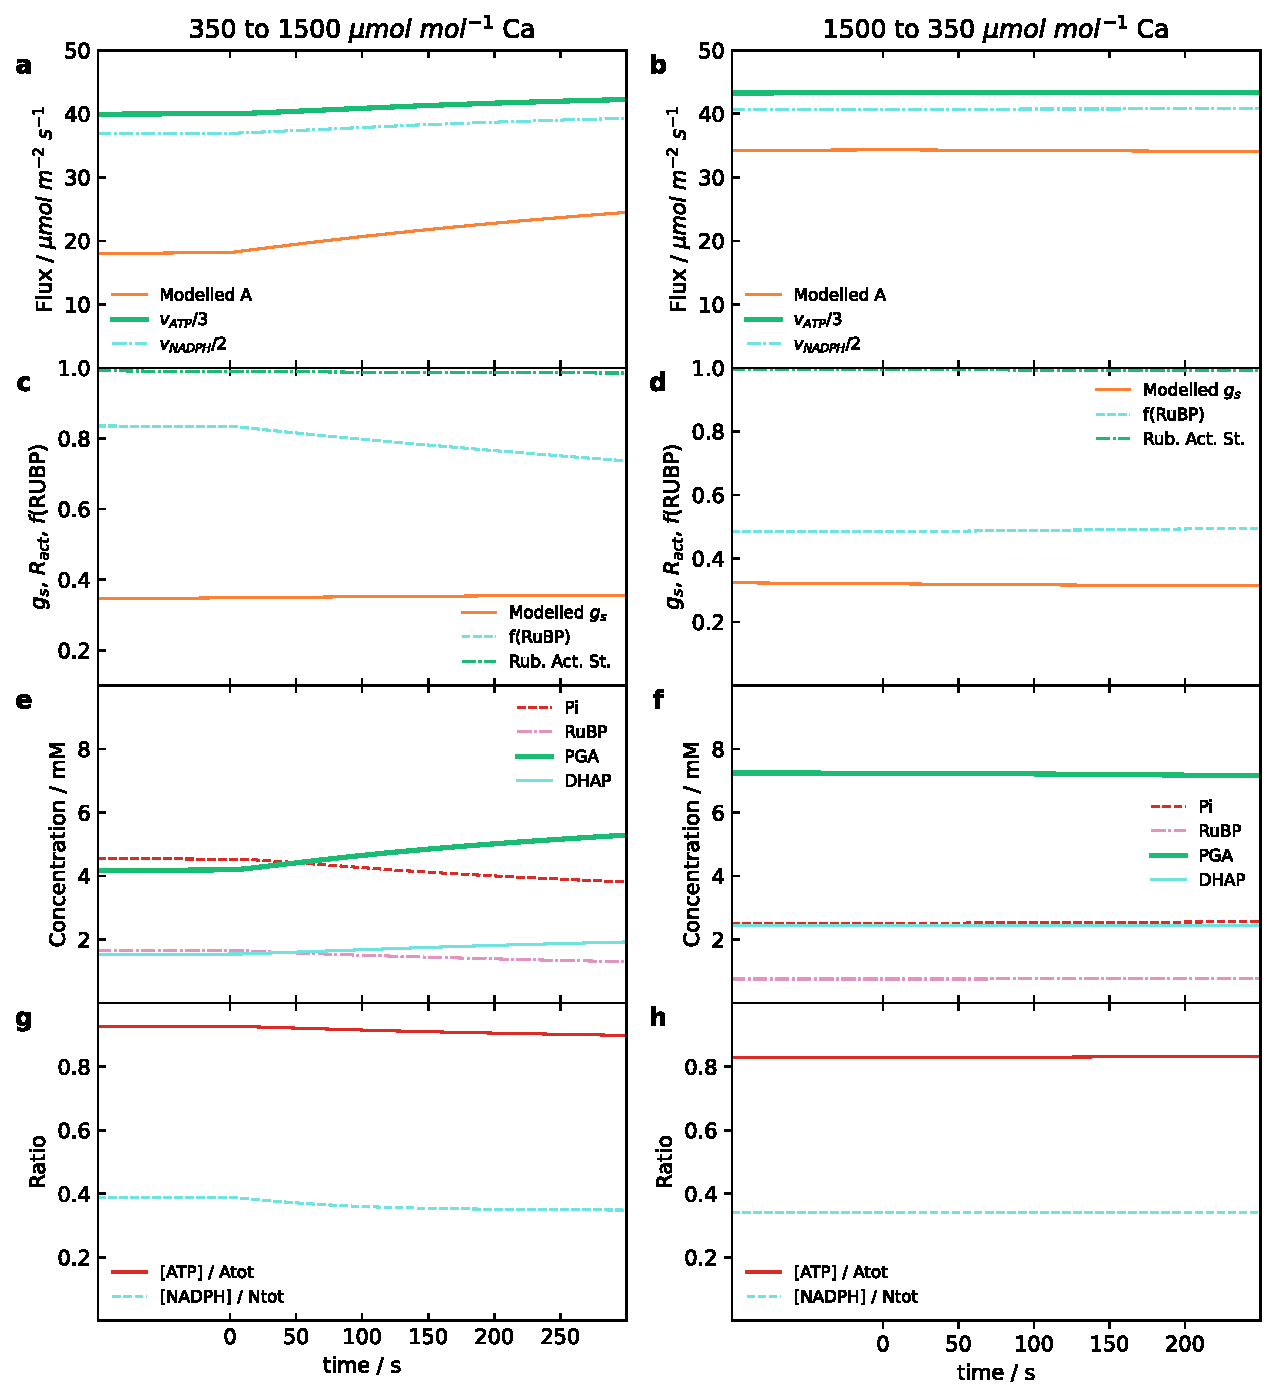
\includegraphics[width=0.7\textwidth]{Figures/Validations/bellasio2019_fig6.pdf}
    \captionvalid{Bellasio2019}{Simulated transition between different \glsentryshort{ca}.}{The simulations were done with an acclimation period of \qty{400}{\second} and a second period that reaches quasi-steady-state at \qty{500}{\second}. Each period is done with a different \glsentryfull{ca} to show a transition. On the left, an ambient to high \glsentryfull{co2} concentration, \qty{350}{\micro\barp} and \qty{1500}{\micro\barp}, transition is done, while on the right the reverse is done. This switch is the zero point on the x-axis. The simulation is run using the default parameters, except \glsentryfull{ppfd} ($=\qty{1500}{\micro\mol\per\square\meter\per\second}$), \glsentryfull{vcmax} ($=\qty{0.18}{\milli\mol\per\meter\squared\per\second}$), \glsentryfull{tau0} ($=\qty{-0.12}{}$), \glsentryfull{Ki} ($=\qty{3600}{\second}$), and \glsentryfull{Kd} ($=\qty{1200}{\second}$). These parameters were chosen to mimic the environment of the experimental work done. The top row shows the \glsentryfull{A}, the \glsentryfull{vatp}, and \glsentryfull{vfnr}. The top-middle row shows the \glsentryfull{gs}, \glsentryfull{Ract}, and \glsentryfull{frubp}. The bottom-middle row shows the \glsentryfull{Pi}, \glsentryfull{rubp}, \glsentryfull{pga}, and \glsentryfull{dhap}. Lastly, the bottom row shows the ratio of \glsentryfull{atp} and \glsentryfull{nadph} to their respective totals. This figure is recreated from figure 6 of the original publication of the Bellasio2019 model~\cite{bellasioGeneralisedDynamicModel2019}.}
    \label{fig:bellasio2019-fig6}
\end{figure}

\begin{figure}
    \centering
    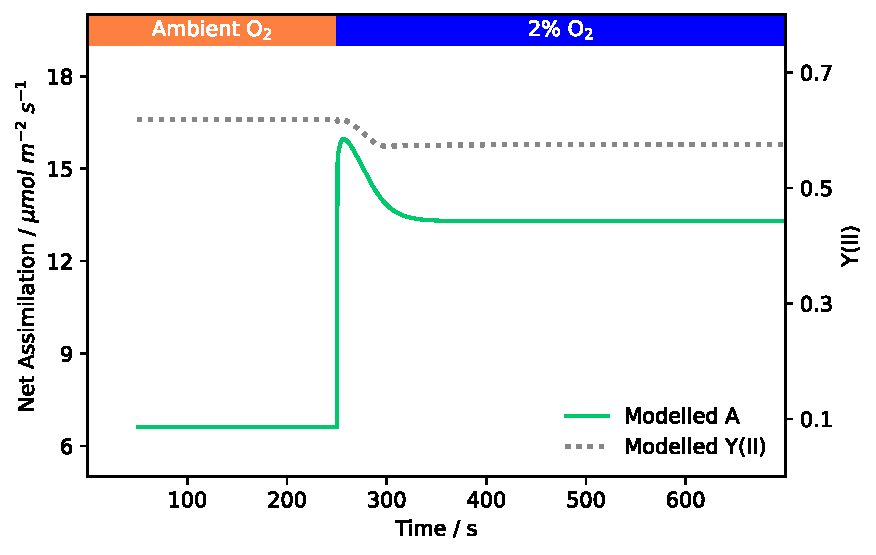
\includegraphics[width=0.7\textwidth]{Figures/Validations/bellasio2019_fig7.pdf}
    \captionvalid{Bellasio2019}{Simulated transition from ambient to low \glsentryshort{o2} concentration.}{Response of the model to a transition from ambient \glsentryfull{o2} concentration (\qty{210000}{\micro\barp}), until steady-state is reached, to low \glsentryfull{o2} concentration (\qty{20000}{\micro\barp}). The simulation is run using the default parameters, except \glsentryfull{ppfd} ($=\qty{300}{\micro\mol\per\square\meter\per\second}$) and \glsentryfull{ca} ($=\qty{200}{\micro\barp}$). Shown in the plot are \glsentryfull{A} (left y-axis) and \glsentryfull{phipsii} (right y-axis). This figure is recreated from figure 6 of the original publication of the Bellasio2019 model~\cite{bellasioGeneralisedDynamicModel2019}. The experimental data could not be plotted, as there was no access to it.}
    \label{fig:bellasio2019-fig7}
\end{figure}

\subsubsection{Fuente2024}

The recreation of the second figure of the Fuente2024 model~\cite{fuenteMathematicalModelSimulate2024} shows a good match to the publication, except for the subfigure at the top right~\figref{fig:fuente2024-fig2}. The \gls{pc_ox} curve fits the same trend as the publication, but is shifted slightly higher. The same applies to the third figure, where all but the \gls{pq_ox} and the \gls{F} curves are near to identical to the publication~\figref{fig:fuente2024-fig3}. Both inaccurate curves are shifted slightly lower in the recreation, especially noticeable in the higher light intensity range.

\begin{figure}
    \centering
    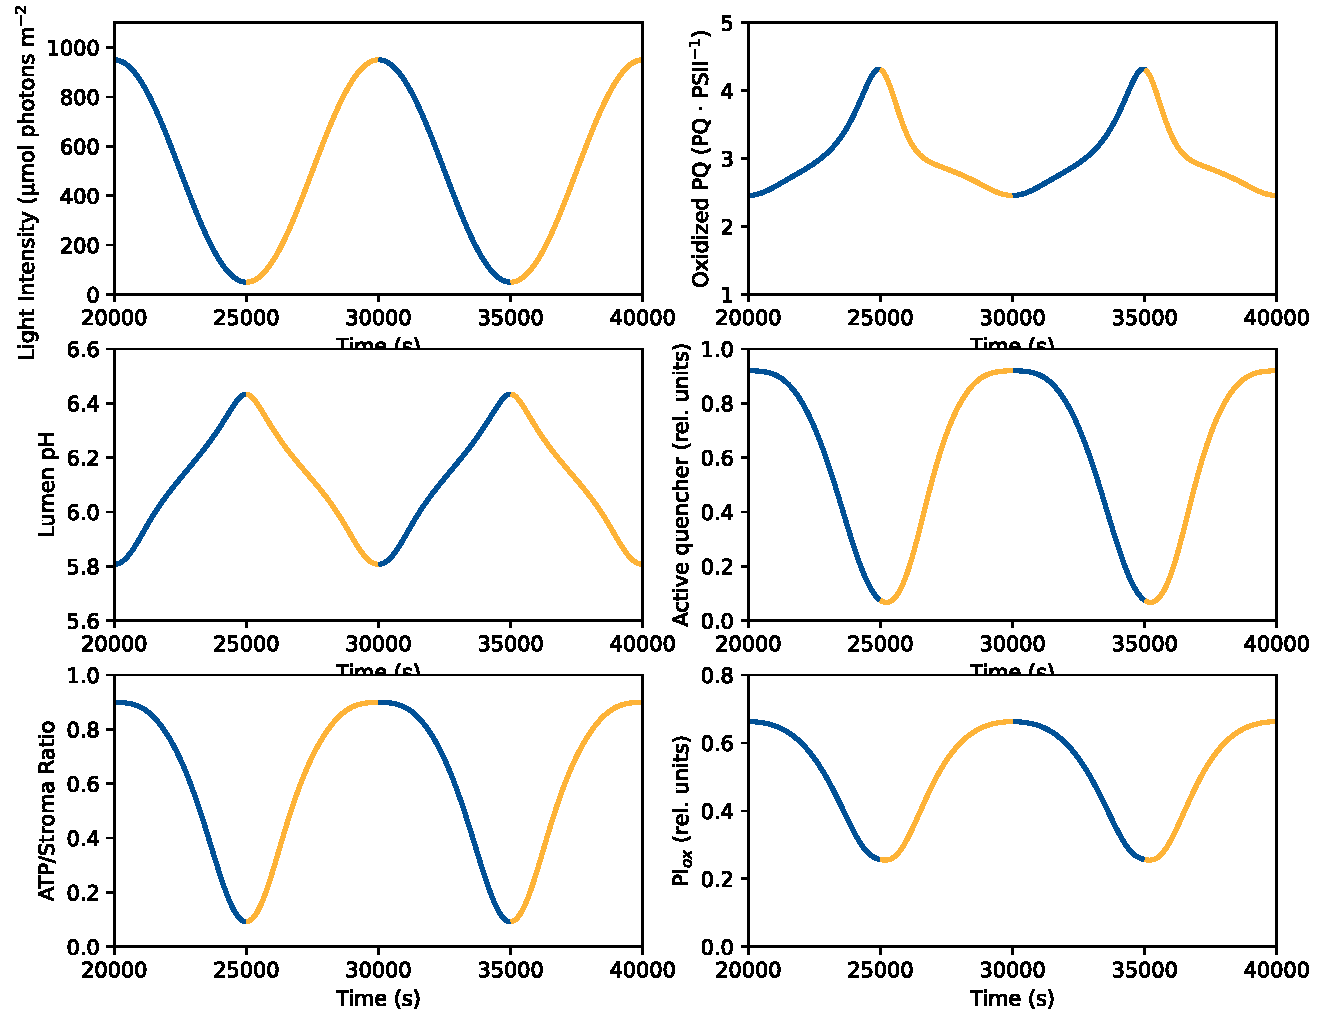
\includegraphics[width=0.7\textwidth]{Figures/Validations/fuente2024_fig2.pdf}
    \captionvalid{Fuente2024}{Results at the end of a long simulation with oscillating light.}{The light intensity used in the simulation is oscillating between \qty{50}{\micro\mol\per\square\meter\per\second} and \qty{950}{\micro\mol\per\square\meter\per\second} with a frequency of \qty[parse-numbers=false]{\frac{1}{10000}}{\per\second}, as seen in the upper left plot. The ascent of light is shown in yellow, while the descent is shown in blue. The results shown are the lumenal pH (middle left), the ratio of \glsentryfull{atp} in the stroma to the \glsentryfull{aptot} (bottom left), the \glsentryfull{pq_ox} (top right), the \glsentryfull{Qactive} (middle right), and the \glsentryfull{psiox} (bottom right). To calculate the lumenal pH, the following equation was used: $\mathrm{pH_{lu}} = -\log_{10}\left(\left[\glsentryshort{h}_\mathrm{lu}\right] \cdot 10^{-6}\right)$. The simulation is run using the default parameters and is simulated to a time of \qty{40000}{\second}, whereas only the last \qty{20000}{\second} are shown in the figure. This figure is recreated from figure 2 of the original publication of the Fuente2024 model~\cite{fuenteMathematicalModelSimulate2024}.}
    \label{fig:fuente2024-fig2}
\end{figure}

\begin{figure}
    \centering
    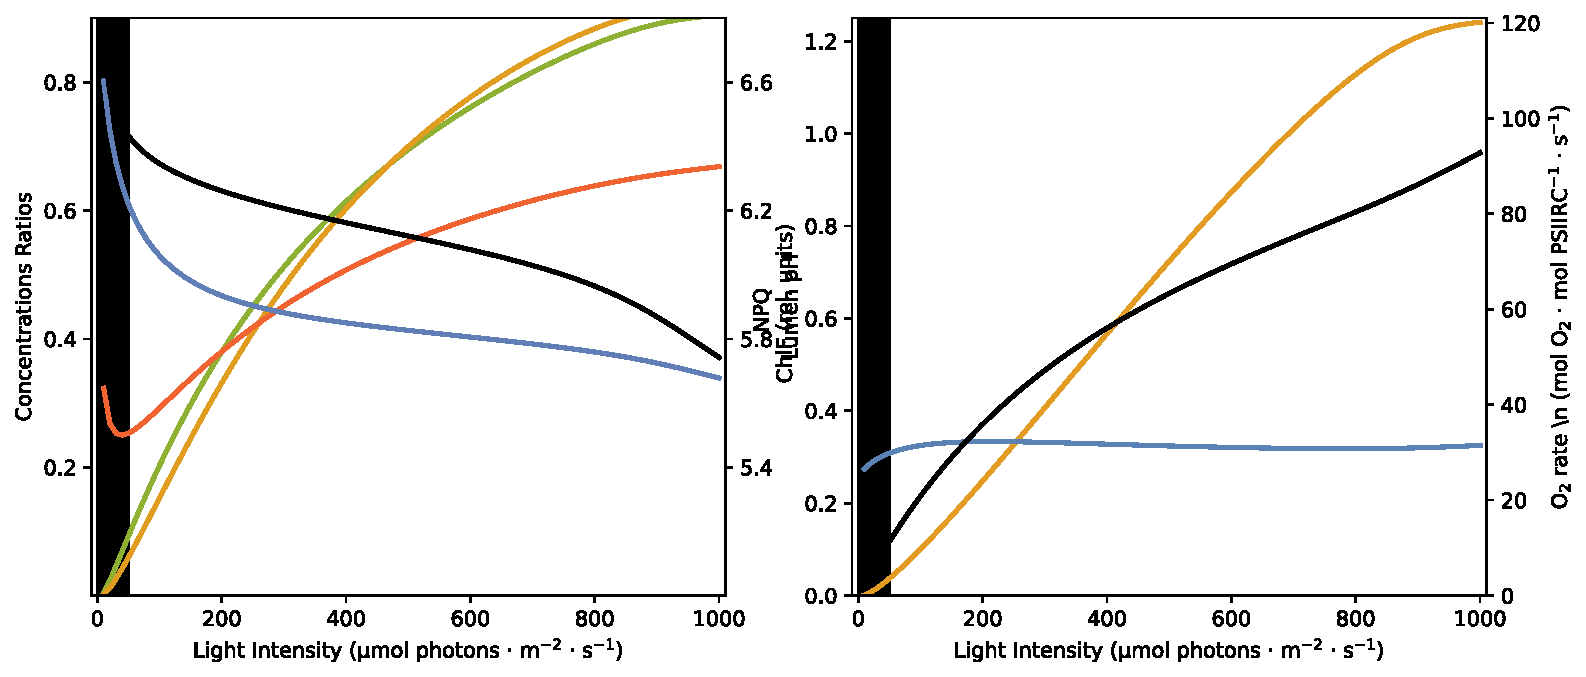
\includegraphics[width=0.7\textwidth]{Figures/Validations/fuente2024_fig3.pdf}
    \captionvalid{Fuente2024}{Steady-state scan of light intensities for several components.}{A steady-state scan of light intensities, from \qty{0}{\micro\mol\per\square\meter\per\second} to \qty{1000}{\micro\mol\per\square\meter\per\second} was done. The left plot shows the ratio of \glsentryfull{atp} in the stroma to the \glsentryfull{aptot} (green), 
    the \glsentryfull{Qactive} (yellow), the lumenal pH (black), the ratio of \glsentryfull{psiox} to the \glsentryfull{psitot} (orange), and the ratio of \glsentryfull{pq_ox} to the \glsentryfull{pqtot}. To calculate the lumenal pH, the following equation was used: $\mathrm{pH_{lu}} = -\log_{10}\left(\left[\glsentryshort{h}_\mathrm{lu}\right] \cdot 10^{-6}\right)$. The right plot shows the \gls{o2} evolution (black), the \glsentryfull{npq} (yellow), and the chlorophyll \glsentryfull{F} (blue), all directly taken from the simulation results. Note the two different y-axis on both plots to showcase different scales. The simulations are run using default parameters, while removing the oscillating light mechanism by setting the amplitude of the oscillation to zero. The light intensity is then inputted as a constant value for each simulation. This figure is recreated from figure 3 of the original publication of the Fuente2024 model~\cite{fuenteMathematicalModelSimulate2024}.}
    \label{fig:fuente2024-fig3}
\end{figure}

The fourth figure shows many similarities to the publications, yet still encompasses issues~\figref{fig:fuente2024-fig4}. The low oscillating light simulation (between \qty{50}{\micro\mol\per\square\meter\per\second} and \qty{150}{\micro\mol\per\square\meter\per\second}) shows a consistent similarity to the publication for the lumenal pH, the ratio of \gls{atp} to \gls{aptot}, and the ratio of \gls{psiox} to \gls{psitot} for all six different frequencies. The curves of the \gls{Qactive} during the low oscillating light stay true to the publication in the lower frequencies (\qty[parse-numbers=false]{\frac{1}{10000}}{\per\second}, \qty[parse-numbers=false]{\frac{1}{1000}}{\per\second}, \qty[parse-numbers=false]{\frac{1}{100}}{\per\second}, the first three rows respectively), while shifting downwards in the higher frequencies (\qty[parse-numbers=false]{}{\per\second}, \qty[parse-numbers=false]{\frac{1}{0.01}}{\per\second}, \qty[parse-numbers=false]{\frac{1}{0.001}}{\per\second}). The recreated \gls{pq_ox} in low oscillation show an upward shift in the lower frequencies, while in the frequencies of \qty[parse-numbers=false]{\frac{1}{0.01}}{\per\second} and \qty[parse-numbers=false]{\frac{1}{0.001}}{\per\second} the shift is ever so slightly down. The high oscillating light simulation (between \qty{50}{\micro\mol\per\square\meter\per\second} and \qty{950}{\micro\mol\per\square\meter\per\second}) is more consistent in its recreation, while still incorporating differences. Both the \gls{pq_ox} and the ratio of \gls{psiox} show an upward shift compared to the publication in all frequencies. In the lower frequencies (\qty[parse-numbers=false]{\frac{1}{10000}}{\per\second}, \qty[parse-numbers=false]{\frac{1}{1000}}{\per\second}, \qty[parse-numbers=false]{\frac{1}{100}}{\per\second}) the lumenal pH, the \gls{Qactive}, and the ratio of \gls{atp} all are identical to the publication. However, in the other frequencies, the latter mentioned is shifted upwards, while the other two down. It has to be noted that most mentioned shifts are minimal, except for the shifts of the \gls{Qactive} in the low frequencies of both oscillating lights and the shifts of the \gls{pq_ox} in the three highest frequencies.

\begin{figure}
    \centering
    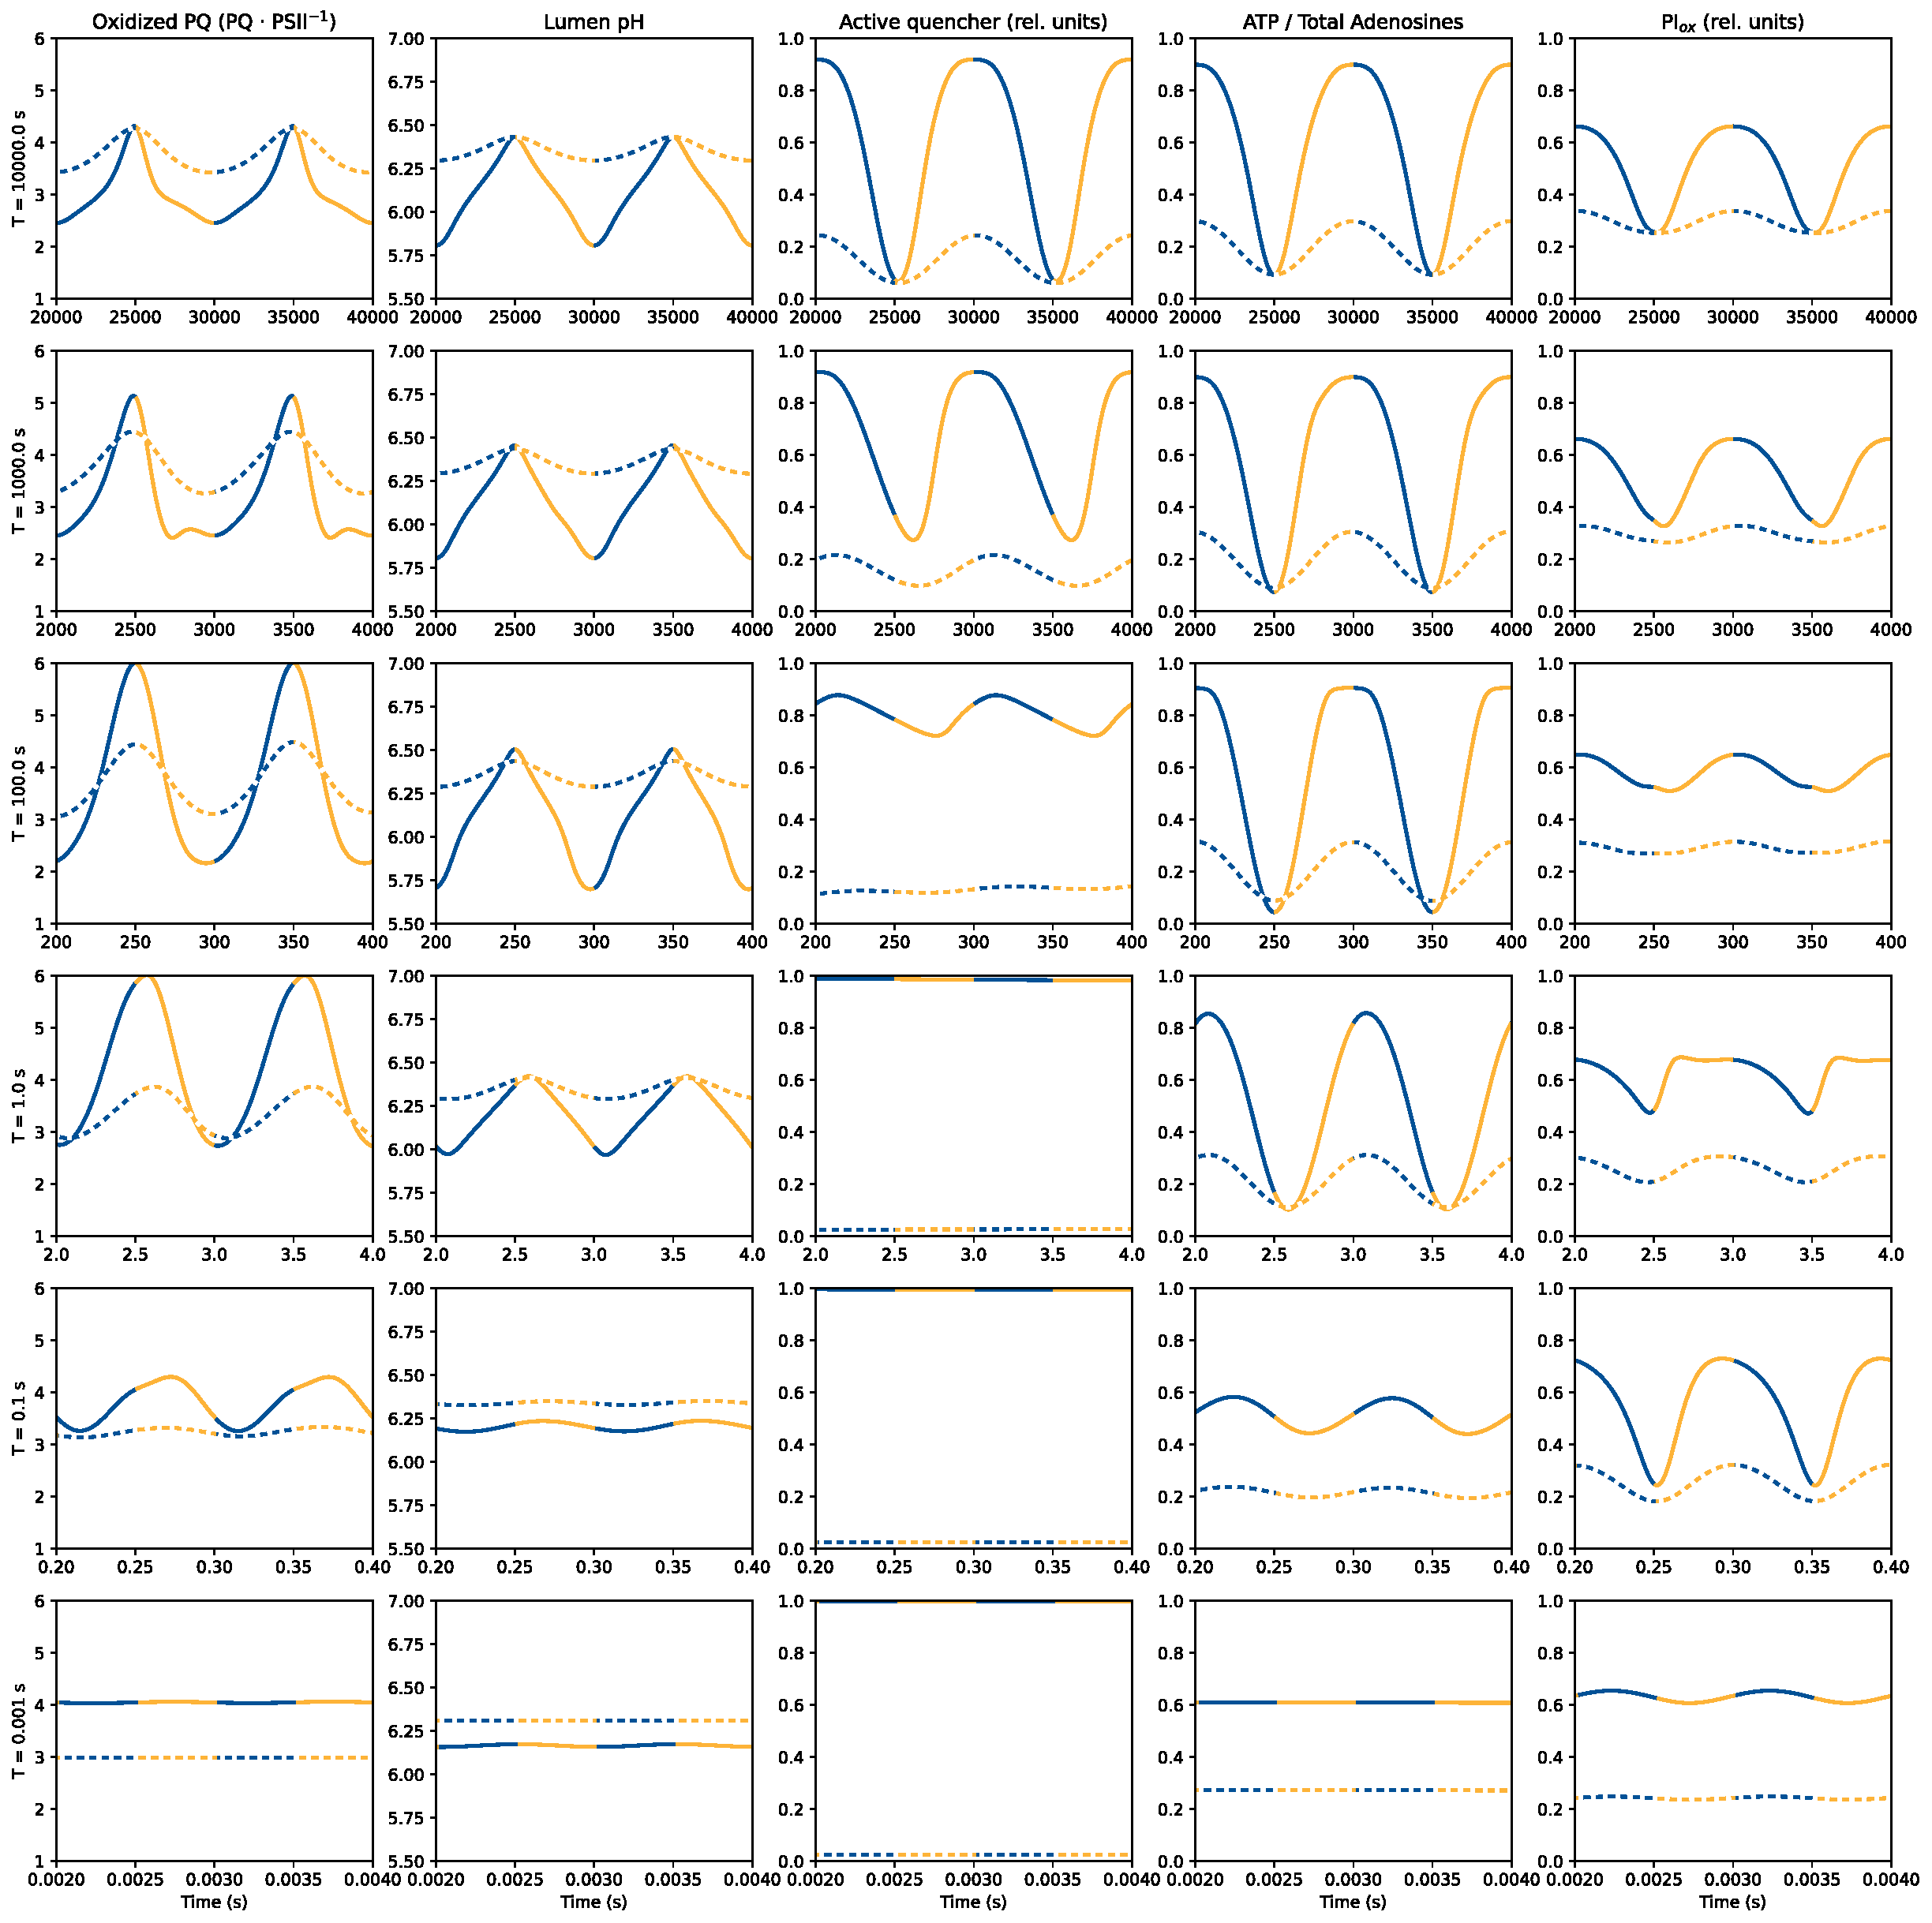
\includegraphics[width=0.7\textwidth]{Figures/Validations/fuente2024_fig4.pdf}
    \captionvalid{Fuente2024}{Results of dependent variables under differing light intensity oscillations conditions.}{Different simulations were done using different settings of the light oscillation. Each row of plots correspond to a different frequency used in the oscillation, with \qty[parse-numbers=false]{\frac{1}{10000}}{\per\second}, \qty[parse-numbers=false]{\frac{1}{1000}}{\per\second}, \qty[parse-numbers=false]{\frac{1}{100}}{\per\second}, \qty[parse-numbers=false]{\frac{1}{1}}{\per\second}, \qty[parse-numbers=false]{1}{\per\second}, and \qty[parse-numbers=false]{\frac{1}{0.001}}{\per\second}, from top to bottom. Additionally, each frequency was simulated twice with differing amplitudes of oscillation. The oscillation was either between \qty{50}{\micro\mol\per\square\meter\per\second} and \qty{950}{\micro\mol\per\square\meter\per\second} (solid) or between \qty{50}{\micro\mol\per\square\meter\per\second} and \qty{150}{\micro\mol\per\square\meter\per\second} (dashed). The ascent of light is shown in yellow, while the descent is shown in blue. The results shown are the \glsentryfull{pq_ox}, the lumenal pH, the \glsentryfull{Qactive}, the ratio of \glsentryfull{atp} in the stroma, and the \glsentryfull{psiox}, from left to right. To calculate the lumenal pH, the following equation was used: $\mathrm{pH_{lu}} = -\log_{10}\left(\left[\glsentryshort{h}_\mathrm{lu}\right] \cdot 10^{-6}\right)$. The simulations are run using the default parameters, while changing the settings of the light oscillation as described. This figure is recreated from figure 4 of the original publication of the Fuente2024 model~\cite{fuenteMathematicalModelSimulate2024}.
    }
    \label{fig:fuente2024-fig4}
\end{figure}

The fifth figure also has similar issues as the last~\figref{fig:fuente2024-fig5}. The \gls{o2} evolution rate is similar to the publication for all the frequencies at the low oscillation, while at the high oscillation it shows an upward shift in the four lower frequencies, while having a downward shift in the other frequencies. The \gls{npq} shows a good match to the publication in both oscillations for the three lower frequencies, while shifting in the higher frequencies. In the low oscillation, the \gls{npq} shifts downwards, while in the high oscillation it shifts upwards. The chlorophyll \gls{F} holds a consistent trend that is comparable to the publication in the low oscillation, and only shows a downward shift in the three highest frequencies. However, the high oscillation results not only show a shift, but also do not follow the correct curvature. In the recreation, the curves are all much more flattened than in the publication, especially in the lower frequencies.

\begin{figure}
    \centering
    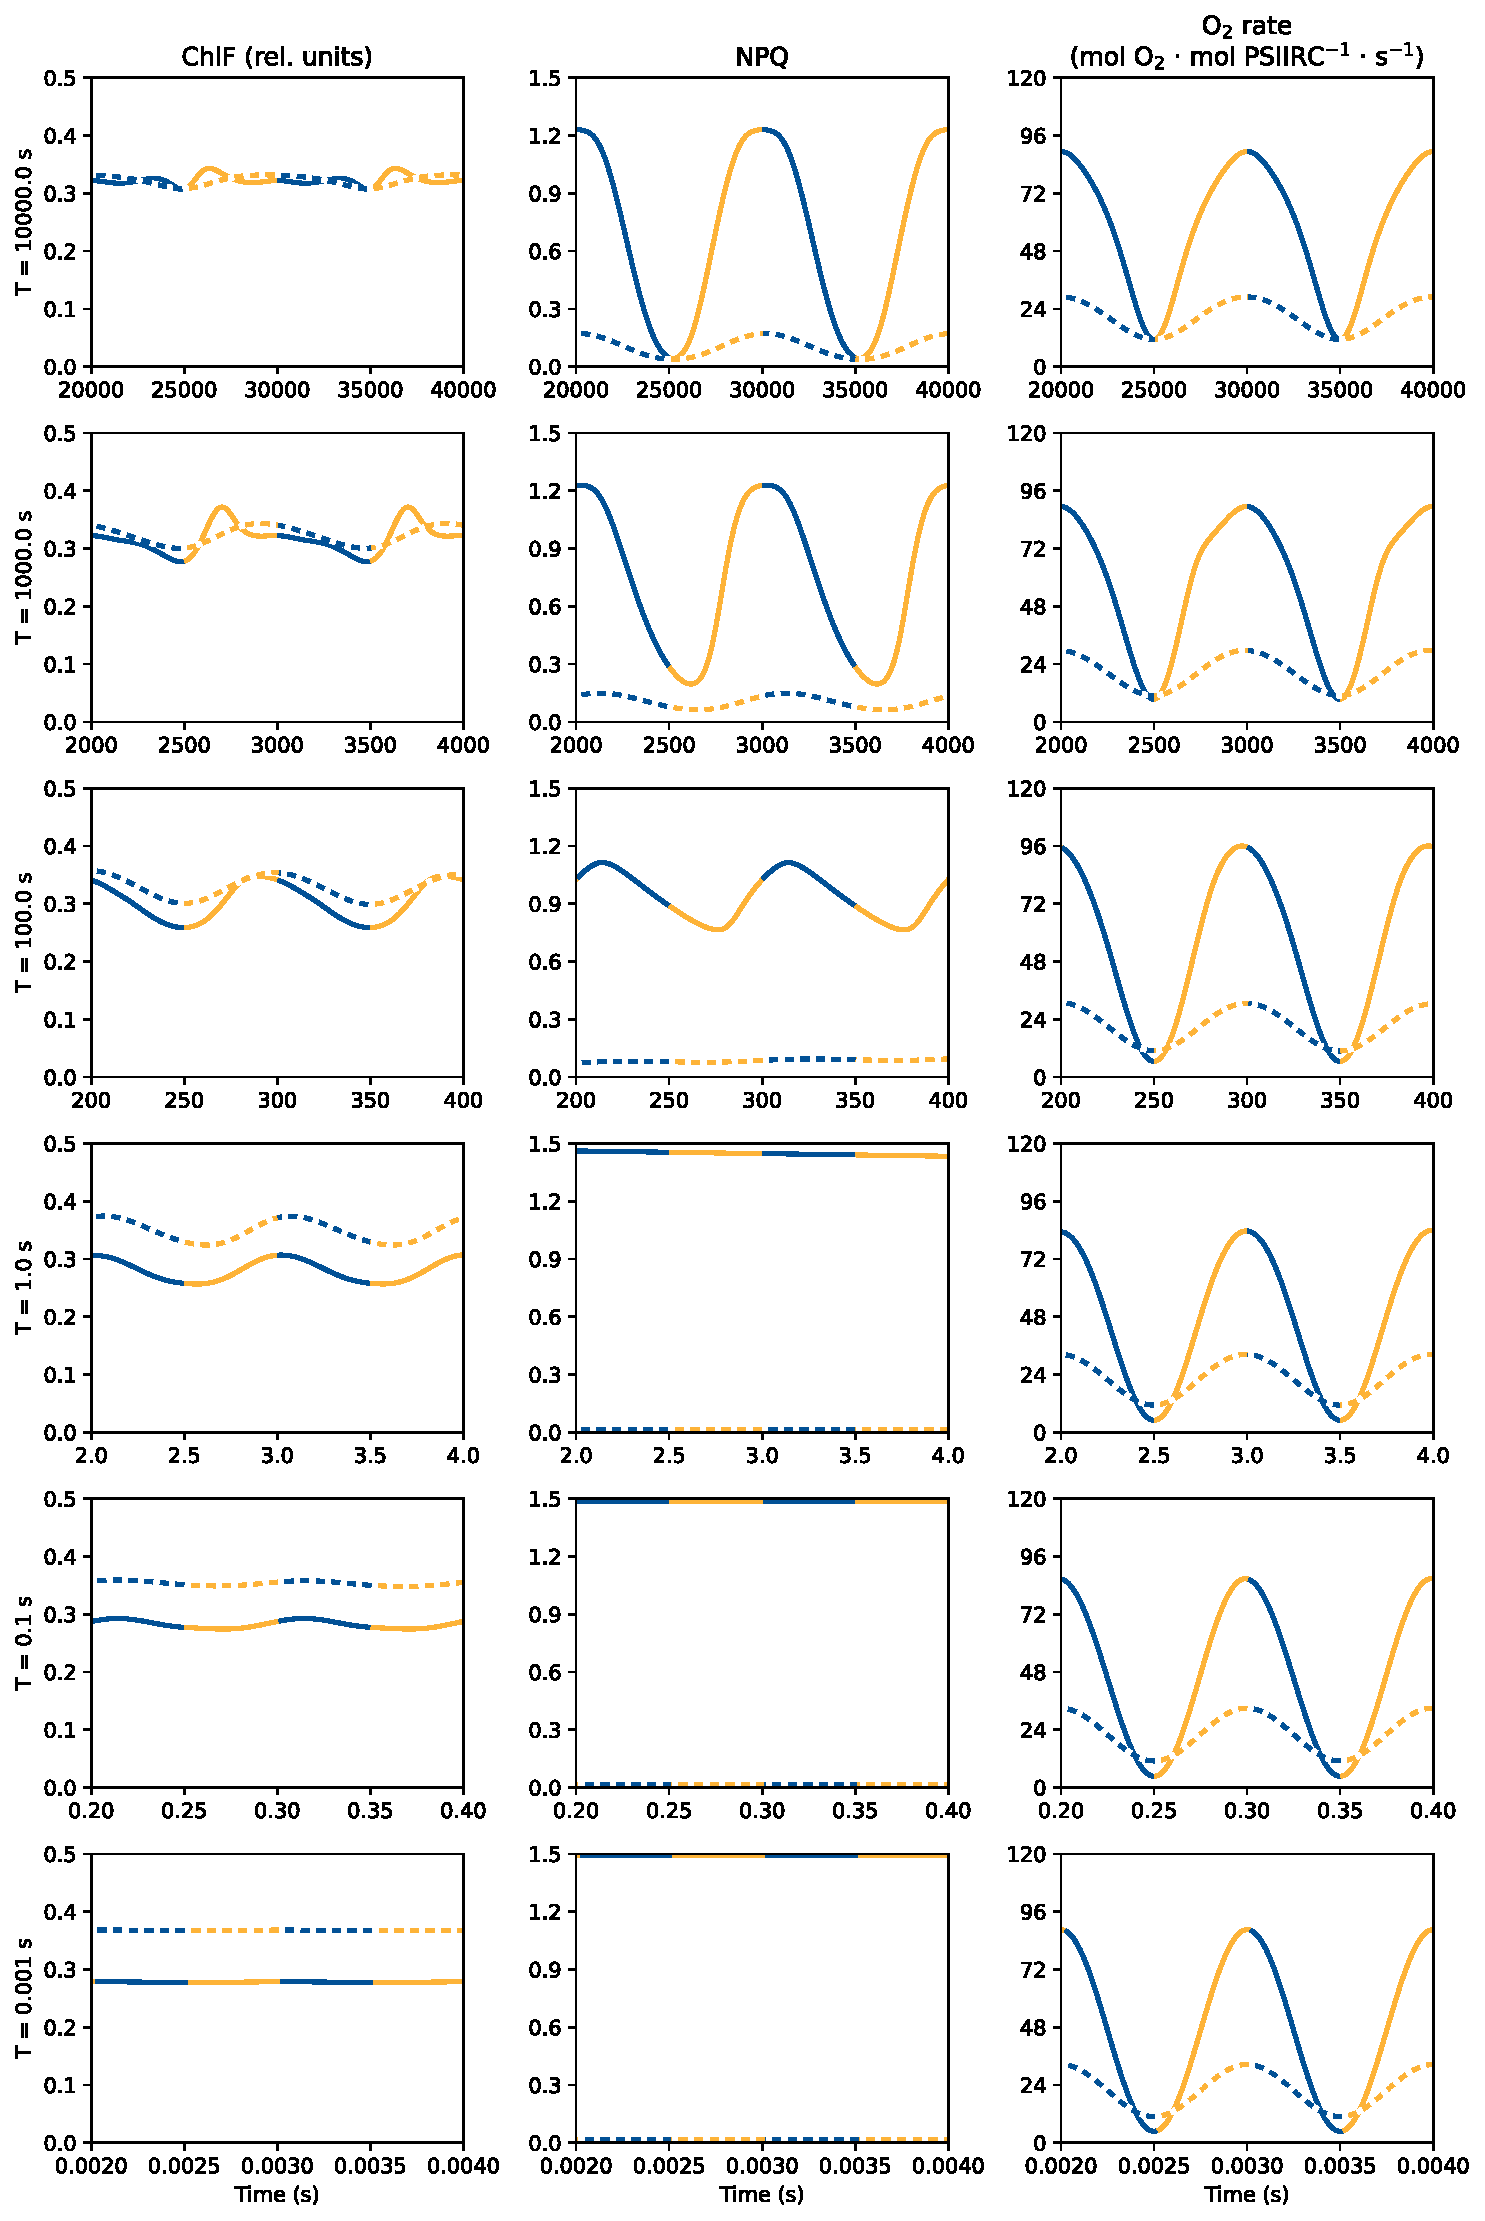
\includegraphics[width=0.7\textwidth]{Figures/Validations/fuente2024_fig5.pdf}
    \captionvalid{Fuente2024}{Results of independent variables under differing light intensity oscillations conditions.}{Different simulations were done using different settings of the light oscillation. Each row of plots correspond to a different frequency used in the oscillation, with \qty[parse-numbers=false]{\frac{1}{10000}}{\per\second}, \qty[parse-numbers=false]{\frac{1}{1000}}{\per\second}, \qty[parse-numbers=false]{\frac{1}{100}}{\per\second}, \qty[parse-numbers=false]{\frac{1}{1}}{\per\second}, \qty[parse-numbers=false]{1}{\per\second}, and \qty[parse-numbers=false]{\frac{1}{0.001}}{\per\second}, from top to bottom. Additionally, each frequency was simulated twice with differing amplitudes of oscillation. The oscillation was either between \qty{50}{\micro\mol\per\square\meter\per\second} and \qty{950}{\micro\mol\per\square\meter\per\second} (solid) or between \qty{50}{\micro\mol\per\square\meter\per\second} and \qty{150}{\micro\mol\per\square\meter\per\second} (dashed). The ascent of light is shown in yellow, while the descent is shown in blue. The results shown are the chlorophyll \glsentryfull{F}, the \glsentryfull{npq}, and the \gls{o2} evolution, from left to right. The simulations are run using the default parameters, while changing the settings of the light oscillation as described. This figure is recreated from figure 5 of the original publication of the Fuente2024 model~\cite{fuenteMathematicalModelSimulate2024}.
    }
    \label{fig:fuente2024-fig5}
\end{figure}

As the prior figures show, the implementation struggled significantly with the \gls{F}, therefore the recreation of the last three figures of the publication, all showing various aspects of this variable, was deemed not possible.

\subsubsection{Li2021}

Some subfigures of the recreation of the third figure of the Li2021 model~\cite{liImpactIonFluxes2021} show a good match to the publication~\figref{fig:li2021-fig3}. In the top row, the \gls{npq} curve of the \gls{wt} with a light intensity of \qty{500}{\micro\mol\per\square\meter\per\second} (first row, third plot) follows the same curve as the other light intensity, a stark rise at the start that forms a peak that slowly falls off to a stable value until the \qty{20}{\minute} mark, and then quickly falls to zero during the dark period. While in the publication, it slowly rises to the stable value and stays there, without first forming a peak, then also quickly drops to zero in the dark. The two last plots could not be reproduced at all, as not enough information was given to be able to recreate them using the model. The first four plots of the bottom row were able to be recreated fully, while the last three show discrepancies with the light intensity of \qty{500}{\micro\mol\per\square\meter\per\second}. As these plots show the difference between the mutant and the \gls{wt} \gls{npq}, the problem of the prior described plot persists in these plots, with the beginning of each curve being shifted upwards compared to the publication.

\begin{figure}
    \centering
    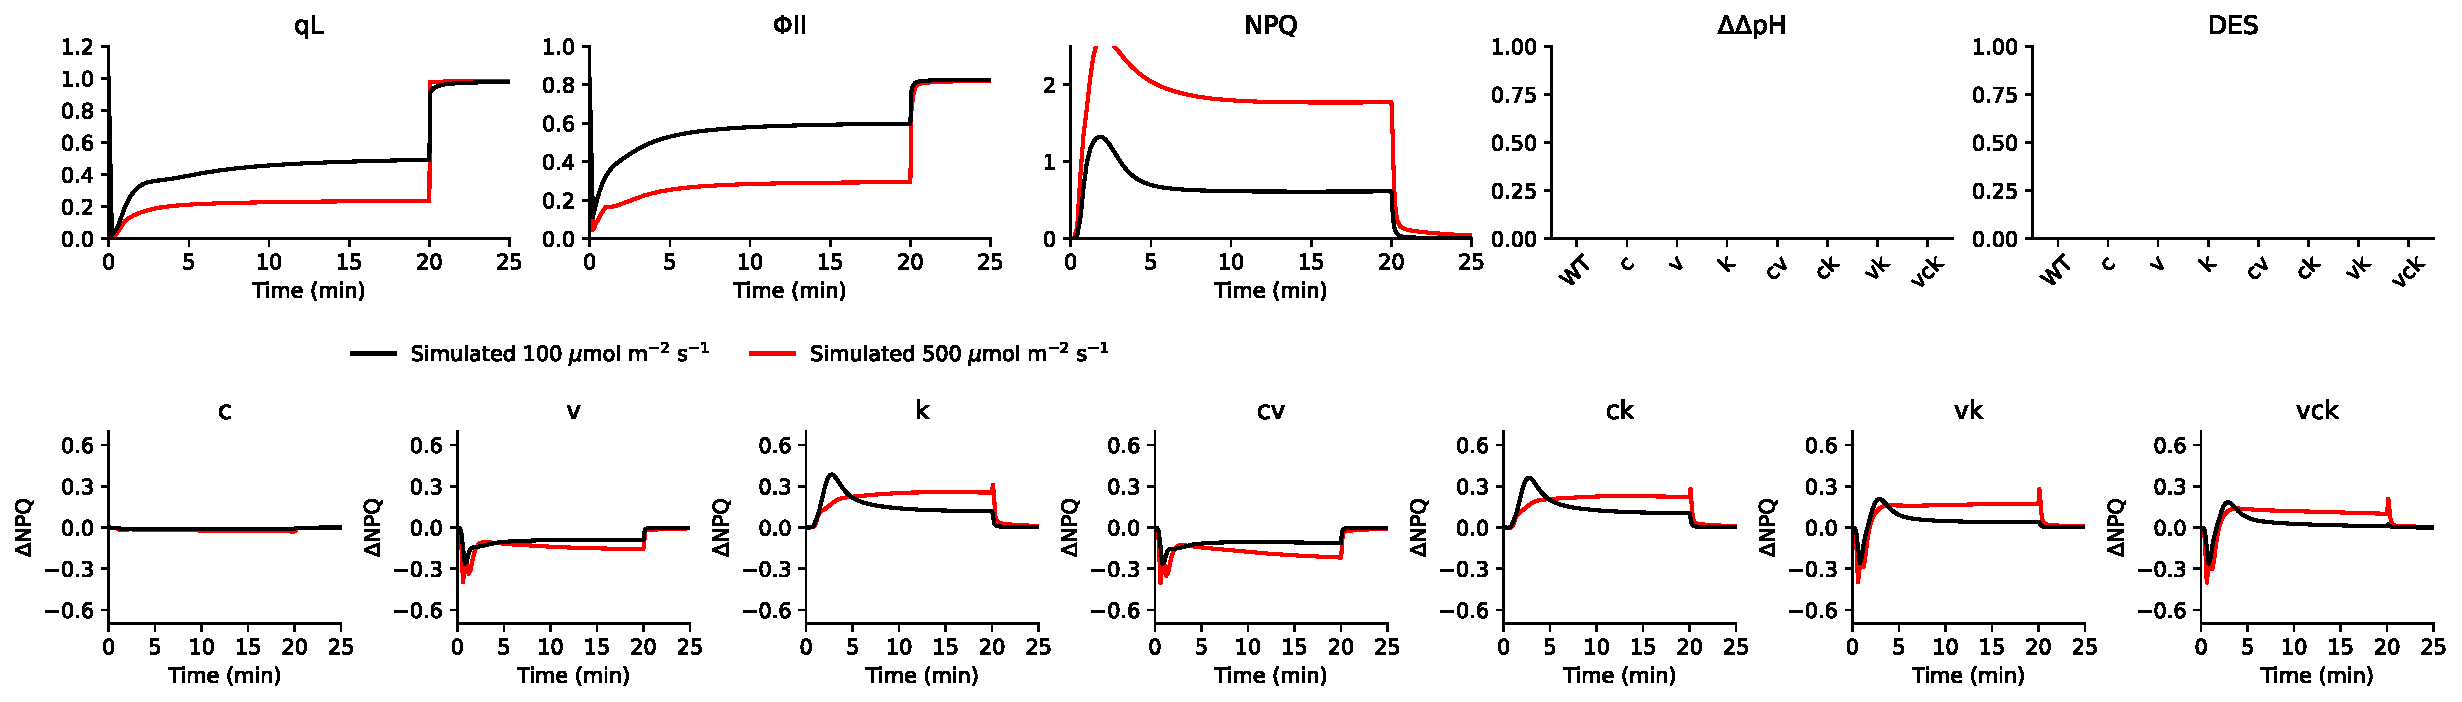
\includegraphics[width=0.7\textwidth]{Figures/Validations/li2021_fig3.pdf}
    \captionvalid{Li2021}{Simulation results of simple light protocol under differing light intensities and mutants.}{
    A simple light protocol consisting of a light period of \qty{20}{\minute}, with a light intensity of \qty{100}{\micro\mol\per\square\meter\per\second} (black) or \qty{500}{\micro\mol\per\square\meter\per\second} (red), and then a dark period of \qty{5}{\minute} was used. This protocol was simulated for several genotypes of \glsentrylong{arabidopsis}, including the \glsentryfull{wt}, and the knockout mutants of the \glsentryfull{clce} (c), \glsentryfull{vccn1} (v), \glsentryfull{kea3} (k), and every variation thereof (cv, ck, vk, vck). The results shown in the top row are the \glsentryfull{qL}, \glsentryfull{phipsii}, and the \glsentryfull{npq} of the \glsentryshort{wt} simulation, for each light intensity. Additionally, there are two empty plots, that are left to make the figure more comparable to the publication, but could not be reproduced. The bottom row shows the difference of \glsentryshort{npq} between the mutant and the \glsentryshort{wt} simulations, for both light intensities. The mutant depicted in the plot is shown in the title of each subplot. The simulations were run using the default parameters, while changing the \glsentryfull{ppfd} to match the light intensities. To create each mutant model, the corresponding rate constant of the rate being knockout was set to zero, for e.g. the rate constant of \glsentryshort{kea3} ($k_\mathrm{KEA}$). This figure is recreated from figure 4 of the original publication of the Li2021 model~\cite{liImpactIonFluxes2021}.
    }
    \label{fig:li2021-fig3}
\end{figure}

The fourth figure was recreated to a good extent, with every plot representing the \qty{100}{\micro\mol\per\square\meter\per\second} light intensity showing a good match to the publication~\figref{fig:li2021-fig4}. However, figure the \qty{500}{\micro\mol\per\square\meter\per\second} light intensity plots show a slight discrepancy, just like in the last figure. All curves follow the approximate trends, while some, like the \gls{dpH} and the \gls{pmf} curves of the \gls{wt} end at too high of a value, or the beginning of the curves show small dips and peaks, like the flux of \glsentryfull{k+lu} in the \gls{vccn1} mutant that rises and forms two peaks, one after another. These inconsistencies can be found throughout the recreated figure, however, only in the plots of the higher light intensity.

\begin{figure}
    \centering
    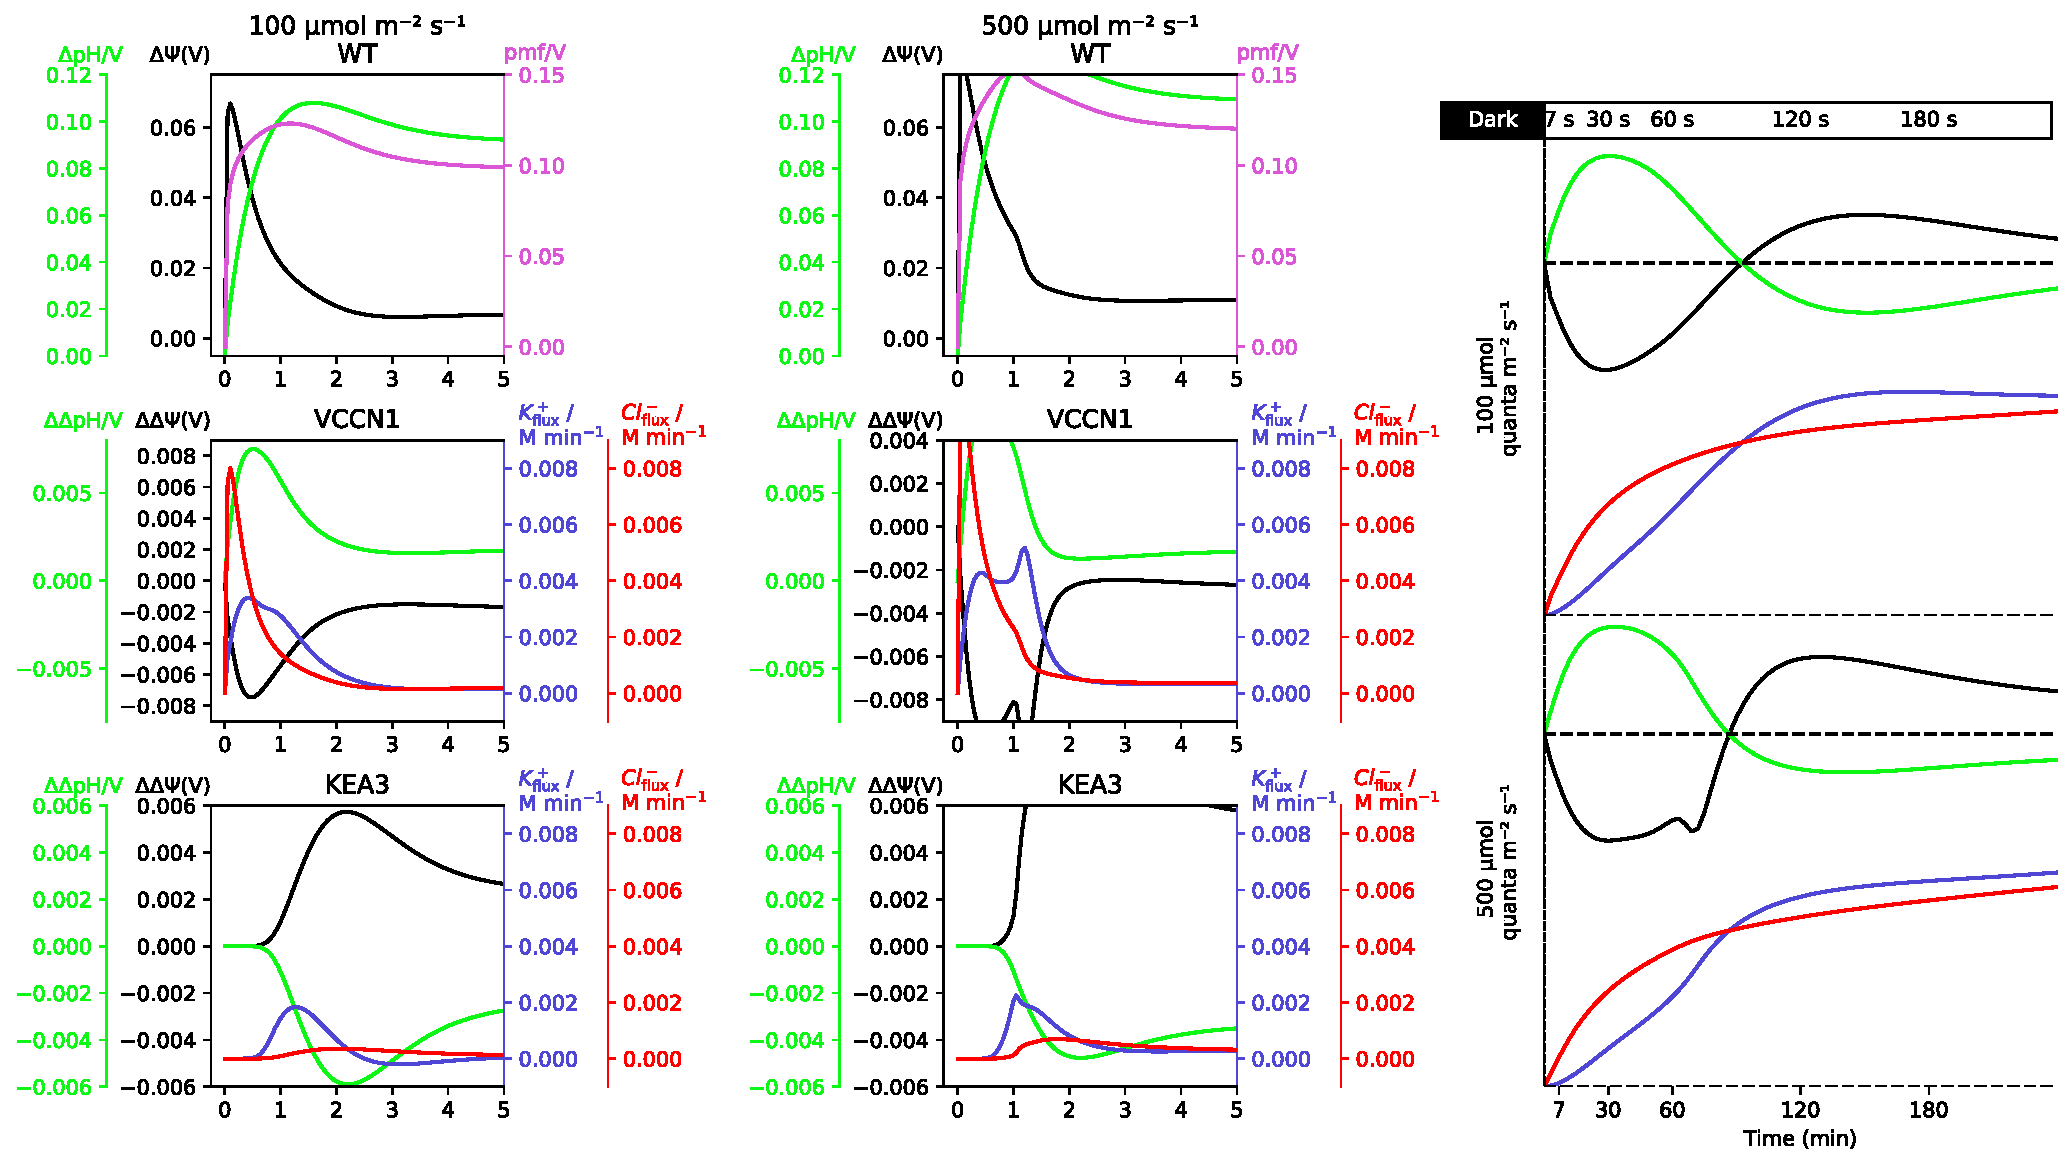
\includegraphics[width=0.7\textwidth]{Figures/Validations/li2021_fig4.pdf}
    \captionvalid{Li2021}{Simulation results of \glsentryshort{kea3} and \glsentryshort{vccn1} knockout mutants under differing light intensities.}{
    The models of the \glsentryfull{wt} (top row), \glsentryfull{vccn1} knockout mutant (middle row),  \glsentryfull{kea3} knockout mutant (bottom row), and the combination of both with the additional \glsentryfull{clce} knockout (right column) were simulated under a light intensity of \qty{100}{\micro\mol\per\square\meter\per\second} (left column, and top row of right column), \qty{500}{\micro\mol\per\square\meter\per\second} (middle column and bottom row of right column). The results shown in the top row of the two left columns are the \glsentryfull{pmf} (pink), the \glsentryfull{dpH} (green), and the \glsentryfull{dpsi} (black), all in Volts, for the \glsentryshort{wt}. In the two last rows of the left columns all curves are differences between the \glsentryshort{wt} and corresponding mutant. These results are the \glsentryfull{dpH} (green) and the \glsentryfull{dpsi} (black) and the fluxes of the \glsentryfull{k+lu} (blue) and \glsentryfull{cl-lu} (red). The fluxes are taken from the model, by getting the right-hand side of each time point of the corresponding \glsentryfull{ode} and by multiplying by 60, to convert from per second to per minute. The same results are plotted on the right column. The simulations were run using the default parameters, while changing the \glsentryfull{ppfd} to match the light intensities. To create each mutant model, the corresponding rate constant of the rate being knockout was set to zero, for e.g. the rate constant of \glsentryshort{kea3} ($k_\mathrm{KEA}$). This figure is recreated from figure 4 of the original publication of the Li2021 model~\cite{liImpactIonFluxes2021}.
    }
    \label{fig:li2021-fig4}
\end{figure}

The recreation of the fifth figure has also some mixed results~\figref{fig:li2021-fig5}. The top row shows a good representation of the first plot, but the second plot has the same problem as the prior plots. The \gls{npq} difference of the \qty{500}{\micro\mol\per\square\meter\per\second} light intensity curve has a too strong rise at the beginning, while getting to the same stable value as the publication. These issues can also be seen in the last plot of the first row, as this plot shows a \qty{2}{\minute} scan of the differences of \gls{npq} at different light intensities. Therefore, all curves in this plot are shifted upwards in comparison to the publication. The first two plots of the middle row show a very good recreation of the publication, while the curve for \gls{vccn1} in the last plot ends at a slightly too high value, compared to the publication. The bottom row starts out with a good match in the first column, but the middle column shows some small mismatches. In both initial plots, the points of the multiplier factor of 10 and 100 are shifted away from the zero point for the \gls{kea3} mutant, while they shift to the zero point for the \gls{vccn1} mutant, compared to the publication. However, the steady-state plots both are a good match to the publication, which cannot be said to the last plot of the bottom row. All the points of the higher multiplier factors are a good match, however, the points of both light intensities of the lower factors are shifted both upwards, where the \qty{500}{\micro\mol\per\square\meter\per\second} light intensity points are shifted much more than the \qty{100}{\micro\mol\per\square\meter\per\second} light intensity points.
\begin{figure}
    \centering
    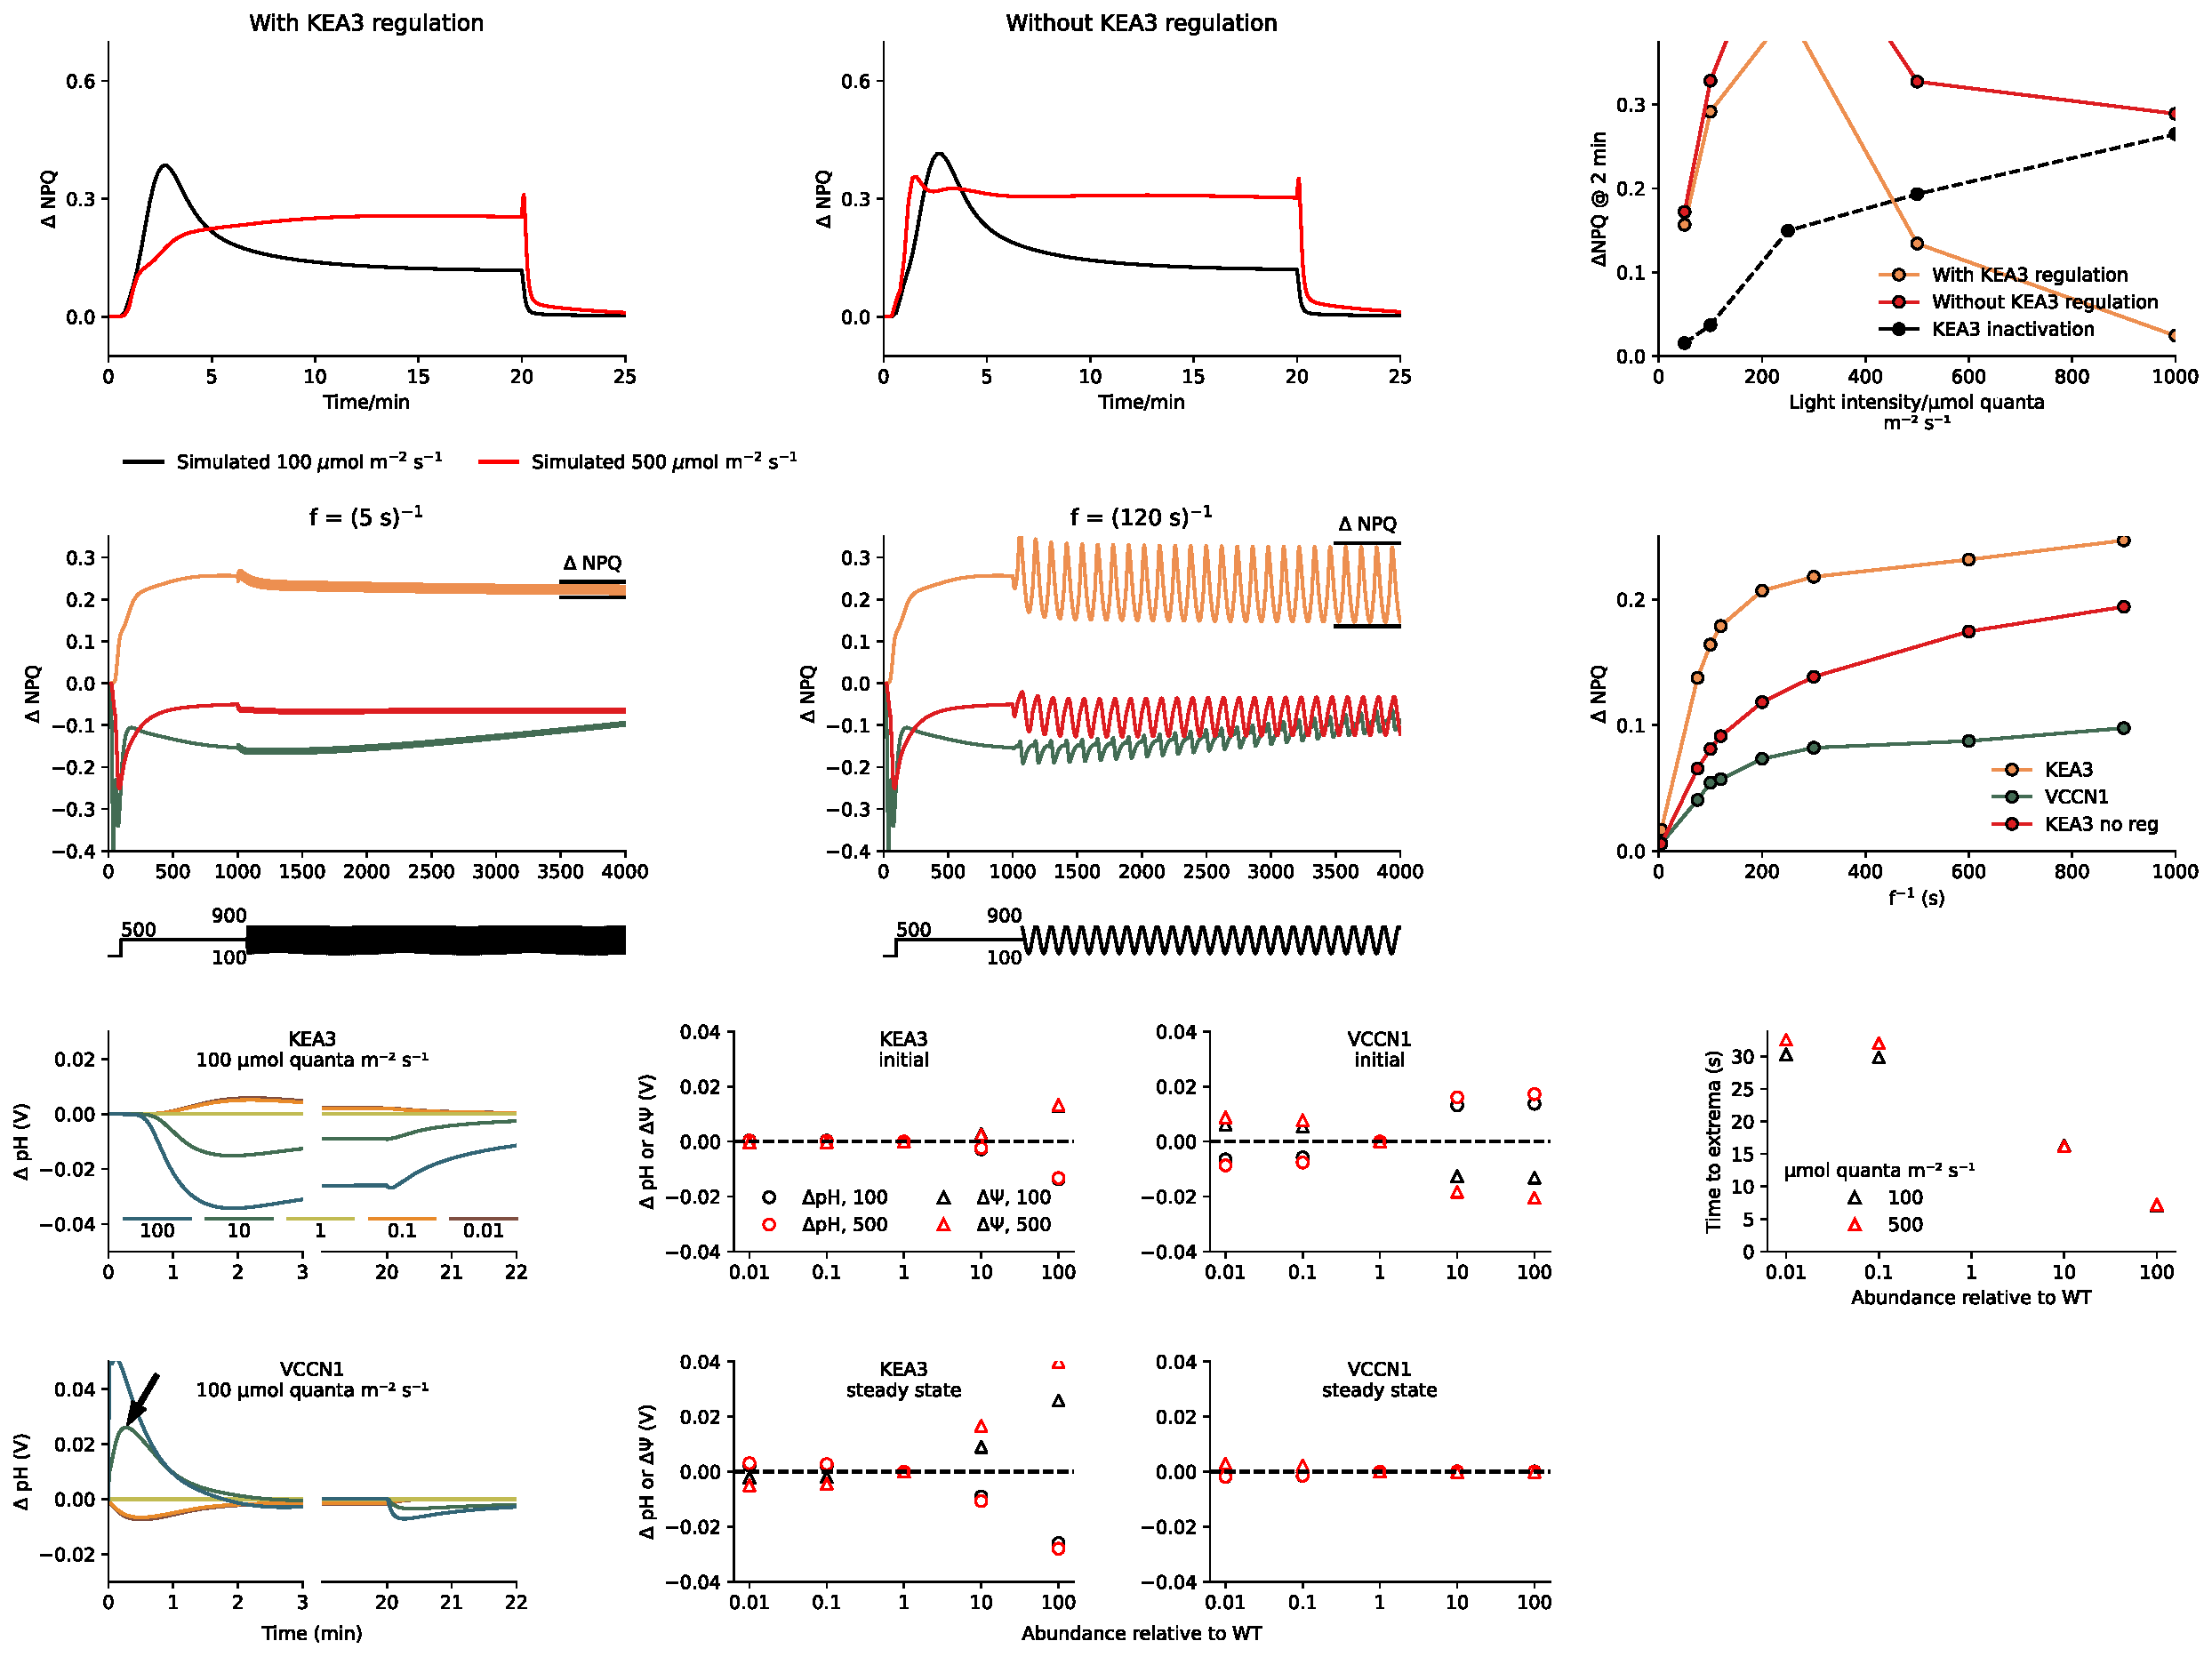
\includegraphics[width=0.7\textwidth]{Figures/Validations/li2021_fig5.pdf}
    \captionvalid{Li2021}{Simulation results of \glsentryshort{kea3} regulation, oscillating light, and different abundances of \glsentryshort{kea3} and \gls{vccn1}.}{
    Three different types of simulation was performed here. The top row shows results of simulations that show the effect of \glsentryfull{kea3} regulation. The first two plots show the results of a simulation following a simple light protocol, with a light period of \qty{20}{\minute} and a dark period of \qty{5}{\minute}. Each plot consists of two simulations, each showing a simulation at either a light intensity of \qty{100}{\micro\mol\per\square\meter\per\second} (black) or \qty{500}{\micro\mol\per\square\meter\per\second} (red). The left plot describes difference of the \glsentryshort{kea3} knockout mutant to the \glsentryshort{wt} simulation, while the right plot describes the difference of a simulation without the \glsentryfull{kea3} regulation mechanism to the \glsentryshort{wt} simulation. To remove the regulation of \glsentryshort{kea3}, the \glsentryfull{qlact} was set to a constant value of one. These plots show the \glsentryfull{npq} over the time series, which is also shown on the right plot, however, as a scan of light intensities at the \qty{2}{\minute} mark. Additionally, a difference curve is also drawn in the plot (black and dashed). The middle row shows the reaction of the model to oscillating light. To simulate this new form of light, a simple sinus curve was used, with the following equation: $\mathrm{PPFD} = \mathrm{PPFD_{base}} + \mathrm{PPFD_{amp}} \cdot \sin\left(2 \pi \cdot \mathrm{f} \cdot t\right)$. In this equation, the $\mathrm{PPFD_{base}}$ shows the value where the oscillation should happen, the $\mathrm{PPFD_{amp}}$ shows the amplitude of the oscillation, and the $\mathrm{f}$ shows the frequency of the oscillation. The two first plots show the difference of \glsentryshort{npq} to the \glsentryshort{wt} of the \glsentryshort{kea3}, \glsentryfull{vccn1}, and without \glsentryshort{kea3} regulation mutants, at two different frequencies. The left at a frequency of \qty[parse-numbers=false]{\frac{1}{5}}{\per\second}, and the right at a frequency of \qty[parse-numbers=false]{\frac{1}{120}}{\per\second}. The simulations were first run to \qty{1000}{\second}
    at a light intensity of \qty{500}{\micro\mol\per\square\meter\per\second} without any oscillation, and then until \qty{4000}{\second} with an oscillation  between \qty{100}{\micro\mol\per\square\meter\per\second} and \qty{900}{\micro\mol\per\square\meter\per\second}. The last plot shows the difference between the extrema of the last wave at varying frequencies of all three mutants. The last row shows the effect of different abundances of \glsentryshort{kea3} and \glsentryshort{vccn1} on the \glsentryfull{dpH} and \glsentryfull{dpsi}. The abundance of either \glsentryshort{kea3} or \glsentryshort{vccn1} was changed by a factor of 100, 10, 1, 0.1, and 0.01, by multiplying the factor to the respective rate constant of the transporter. The simulations run follow the same light protocol as the first row, show the difference of \glsentryshort{dpH} to the normal abundance (1) as a time series for \qty{100}{\micro\mol\per\square\meter\per\second}. The four plots in the middle show the initial and steady-state values of \glsentryshort{dpH} (circles) and \glsentryshort{dpsi} (triangles) at \qty{100}{\micro\mol\per\square\meter\per\second} (black) and \qty{500}{\micro\mol\per\square\meter\per\second} (red), for each abundance, also as a difference to the normal abundance. The initial values were taken as a difference of the value at \qty{50}{\second} to the start of the respective simulation, while the steady-state values were taken at \qty{20}{\minute}. The last plot on the right shows the time it took to reach the extrema of the \glsentryshort{vccn1} abundance time series. An example is marked as an arrow in the bottom left plot. The time point of the extrema of both light intensities is then plotted. All simulations named here were run using the default parameters, unless stated otherwise. To create each mutant model, the corresponding rate constant of the rate being knockout was set to zero, for e.g. the rate constant of \glsentryshort{kea3} ($k_\mathrm{KEA}$). This figure is recreated from figure 5 of the original publication of the Li2021 model~\cite{liImpactIonFluxes2021}.
    }
    \label{fig:li2021-fig5}
\end{figure}

\subsubsection{Matuszynska2016}

In the recreation of the fourth figure of the Matuszynska2016 model~\cite{matuszynskaMathematicalModelNonphotochemical2016}, all three plots show a very good match to the publication~\figref{fig:matuszynska2016-fig4}. As access to the experimental data was possible was given, the experimental values were also plotted. The only thing to note, is that these data points had to be shifted on the x-axis to fit the actual peaks of the simulation. It is assumed that, that was also done for the publication, which is why it was done here.

\begin{figure}
    \centering
    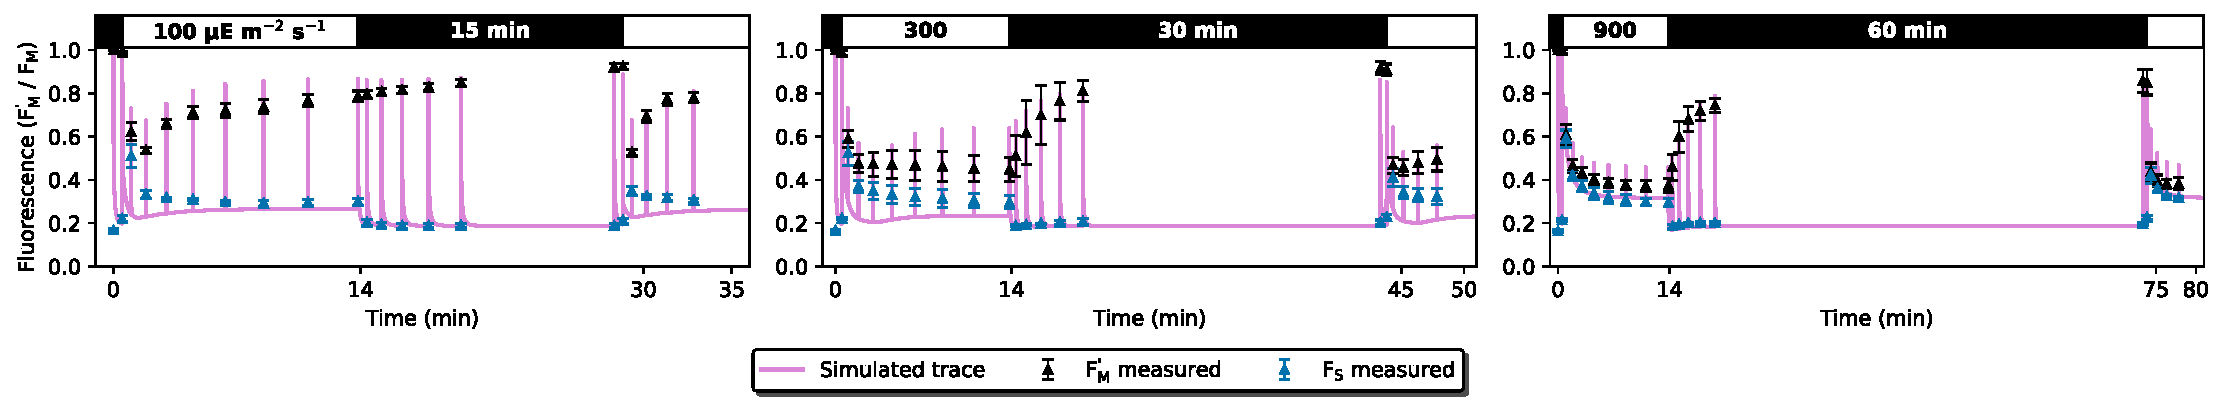
\includegraphics[width=\textwidth]{Figures/Validations/matuszynska2016_fig4.pdf}
    \captionvalid{Matuszynska2016}{Experimental and simulated \glsentryshort{pam} protocol with three different light levels and durations of \glsentrylong{arabidopsis}.}{A \glsentryfull{pam} protocol was done using \glsentrylong{arabidopsis} plants, with three different light levels and durations. The protocols start with a saturating pulse, followed by a dark period of \qty{30}{\second}, then a light period of \qty{14}{\minute} that starts with a saturating pulse and continues with 7 additional ones, all an accumulative 20 seconds apart ($+$\qty{30}{\second}, $+$\qty{50}{\second}, $+$\qty{70}{\second}, etc. from the start of the period). Then another dark period of differing lengths, also starting with a saturating pulse and going along with 5 additional ones, also an accumulative 20 seconds apart. To end the protocol, a final light period of \qty{5}{\minute}, with a saturating pulse to start and 4 additional ones, also an accumulative 20 seconds apart. The three different protocols only differ in the light intensities of the light periods and the duration of the second dark period. The first protocol, shown on the left, has a light intensity of \qty{100}{\micro\mol\per\square\meter\per\second} and a second dark period of \qty{15}{\minute}. The second protocol, shown in the middle, has a light intensity of \qty{300}{\micro\mol\per\square\meter\per\second} and a second dark period of \qty{30}{\minute}. The third protocol, shown on the right, has a light intensity of \qty{900}{\micro\mol\per\square\meter\per\second} and a second dark period of \qty{60}{\minute}. The experimental values shown, are the base \glsentryfull{F} (blue) and the \glsentryfull{Fm} (black). Three replicates for each measurement were done, but only the mean values and standard deviation are shown. The data was taken from the original publication~\cite{matuszynskaMathematicalModelNonphotochemical2016}, therefore all the other meta-information is to be read there. The simulation (pink) was done using the default parameters and changing the \glsentryfull{ppfd} to match the light intensities of the protocols and saturating pulses of \qty{2000}{\micro\mol\per\square\meter\per\second}. Additionally, the \glsentryshort{ppfd} was converted to an internal activation rate, that was calibrated to three light intensities of \glsentryshort{arabidopsis}. This was done by following equation: $\mathrm{Light} = 0.0005833 \cdot \mathrm{PPFD}^2 + 0.2667 \cdot \mathrm{PPFD} + 187.5$. This figure is recreated from figure 4 of the original publication of the Matuszynska2016 model~\cite{matuszynskaMathematicalModelNonphotochemical2016}.}
    \label{fig:matuszynska2016-fig4}
\end{figure}

The fifth figure consists of two different subfigures, the top showing a striking similarity to the publication except for the lumenal pH curve of \qty{300}{\micro\mol\per\square\meter\per\second} and \qty{900}{\micro\mol\per\square\meter\per\second} light intensity, both shifted slightly downwards in the recreation~\figref{fig:matuszynska2016-fig5}. However, both show the same trend through the time series. The phase plane trajectory on the other hand, shows only a slight similarity. The highest lumenal pH reaches at higher \gls{Q} activity is that of 7, while in the publication it is near to 8. Overall, the trajectories are all shifted downwards in the recreation, except for the trajectory of \qty{100}{\micro\mol\per\square\meter\per\second}, which shows the most similarity to the publication. On top of that, the steady-state values are also all shifted downwards and the points attributed to the light intensities, are not in the same places as in the publication.

\begin{figure}
    \centering
    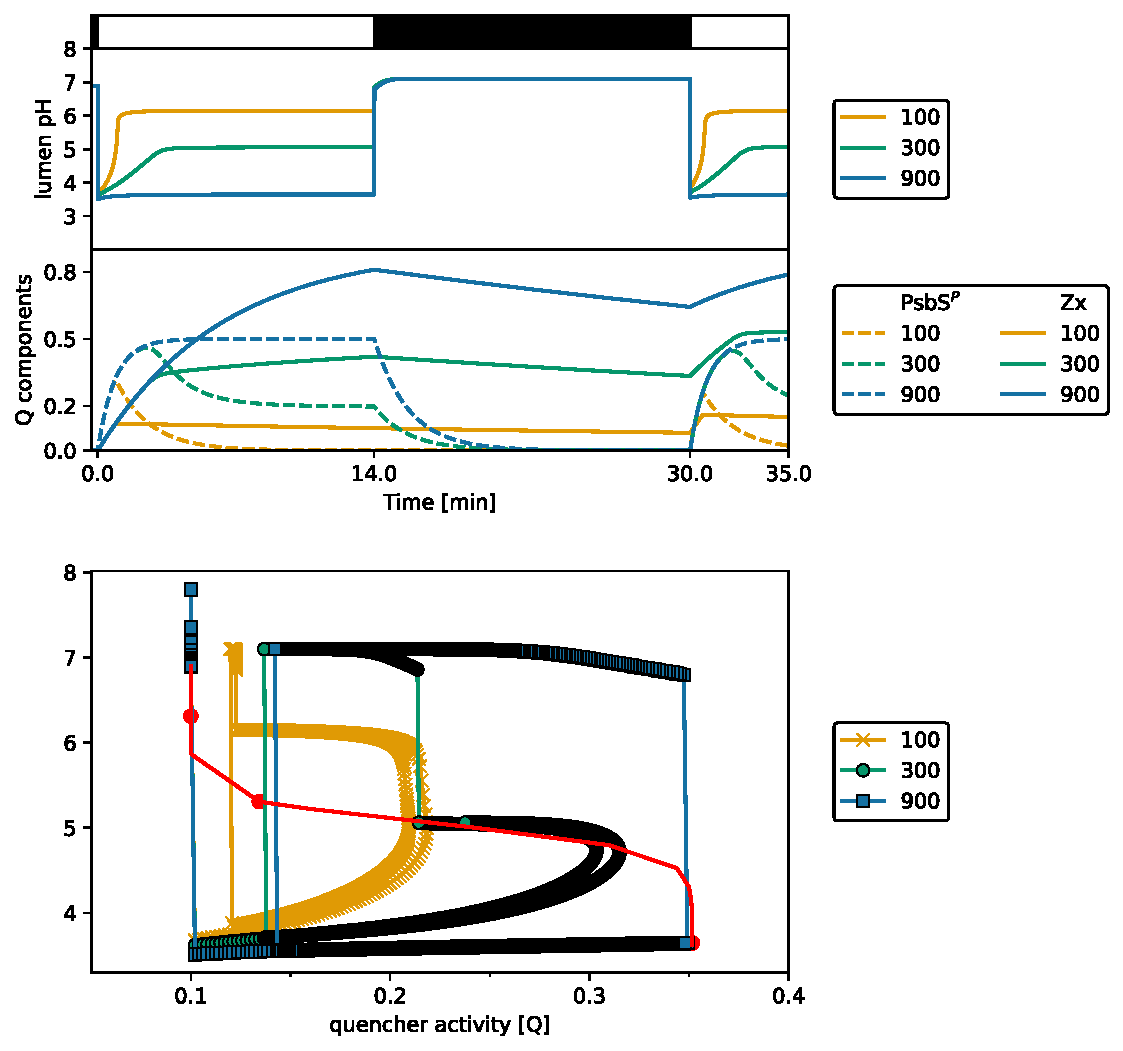
\includegraphics[width=0.7\textwidth]{Figures/Validations/matuszynska2016_fig5.pdf}
    \captionvalid{Matuszynska2016}{Visualisation of lumenal pH and quencher components in response to different light intensities.}{A protocol of dark and light periods was used to simulate the model at three different light intensities. The protocol starts with a dark period of \qty{30}{\second}, followed by a light period of \qty{14}{\minute}, then another dark period of \qty{16}{\minute}, and ending with a final light period of \qty{5}{\minute}. The three different light intensities used in the light periods were \qty{100}{\micro\mol\per\square\meter\per\second} (yellow), \qty{300}{\micro\mol\per\square\meter\per\second} (green), and \qty{900}{\micro\mol\per\square\meter\per\second} (blue). The time series of each simulation is shown in the top plot, for the lumenal pH and the concentration of the quencher components \glsentryfull{psbsp} and \glsentryfull{zx}. The bottom plot shows a phase plane trajectory of the \glsentryfull{Q} and the lumenal pH for each light intensity. Each simulation was done with the default parameters of the model, whereas the light intensities were inputted using the conversion of \glsentryfull{ppfd} to an internal activation rate for \glsentrylong{arabidopsis} by following equation: $\mathrm{Light} = 0.0005833 \cdot \mathrm{PPFD}^2 + 0.2667 \cdot \mathrm{PPFD} + 187.5$. This figure is recreated from figure 5 of the original publication of the Matuszynska2016 model~\cite{matuszynskaMathematicalModelNonphotochemical2016}.}
    \label{fig:matuszynska2016-fig5}
\end{figure}

The last figure could also be successfully recreated, with only two small discrepancies~\figref{fig:matuszynska2016-fig6}. The first is that the first value of the \gls{phipsii} curve in the recreation is much lower than in the publication and the second is that the recreation misses the last value of the \gls{phipsii} curve. Other than that, both simulation results and experimental data show a very good match to the publication. Here it should also be noted that the experimental data was shifted on the x-axis to fit the peaks of the simulation, as was done for the prior figure.

\begin{figure}
    \centering
    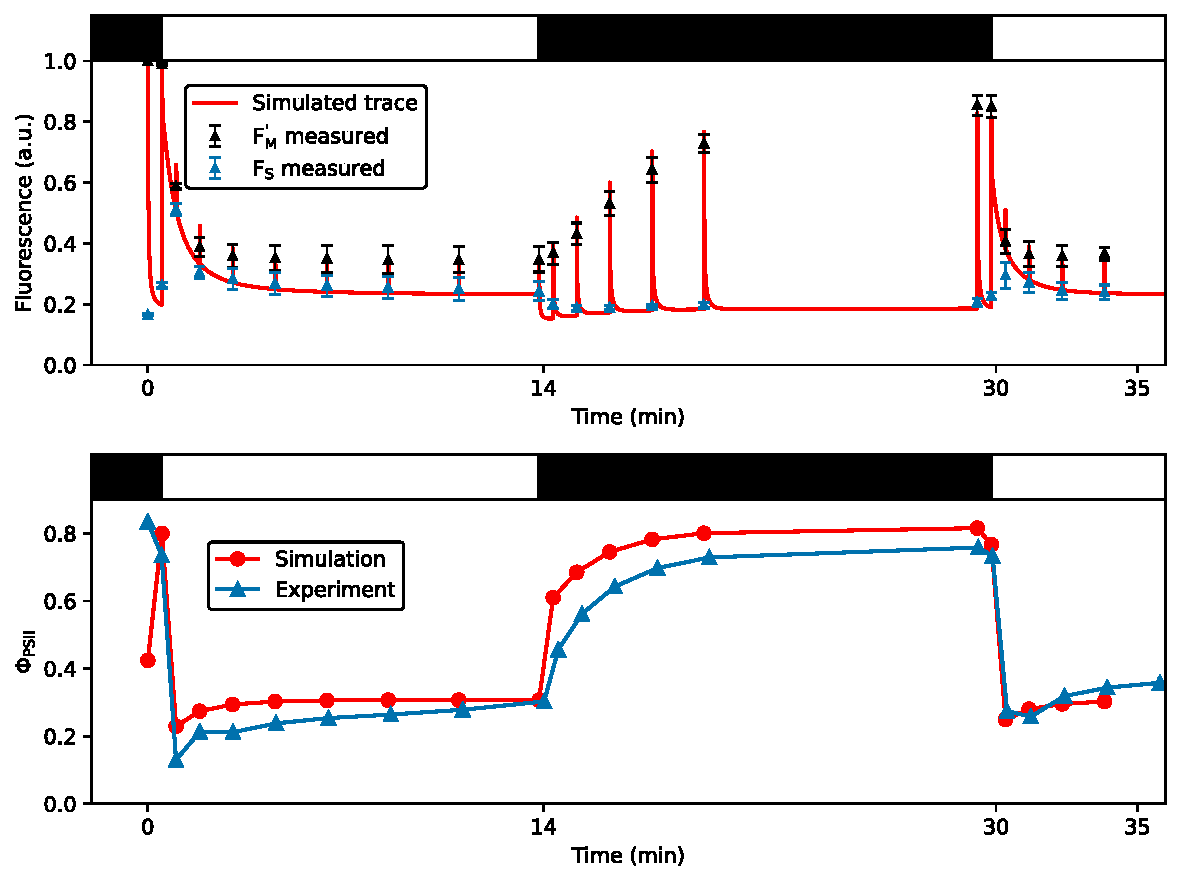
\includegraphics[width=0.7\textwidth]{Figures/Validations/matuszynska2016_fig6.pdf}
    \captionvalid{Matuszynska2016}{Experimental and simulated \glsentryshort{pam} protocol of \glsentrylong{epipremnum}.}{A \glsentryfull{pam} protocol was done using \glsentrylong{epipremnum} plants that starts with a saturating pulse, followed by a dark period of \qty{30}{\second}, then a light period of \qty{14}{\minute} of a light intensity of that starts with a saturating pulse and continues with 7 additional ones, all an accumulative 20 seconds apart ($+$\qty{30}{\second}, $+$\qty{50}{\second}, $+$\qty{70}{\second}, etc. from the start of the period). Then another dark period of \qty{16}{\minute}, also starting with a saturating pulse and going along with 5 additional ones, also an accumulative 20 seconds apart, except for the last that occurs \qty{30}{\second}. To end the protocol, a final light period of \qty{5}{\minute}, with a saturating pulse to start and 4 additional ones, also an accumulative 20 seconds apart. The light intensity used for the light periods is \qty{100}{\micro\mol\per\square\meter\per\second}, while the dark is \qty{0}{\micro\mol\per\square\meter\per\second}. The experimental values shown, are the base \glsentryfull{F} (blue) and the \glsentryfull{Fm} (black) at the top and the \glsentryfull{phipsii} at the bottom. Three replicates for each measurement were done, but only the mean values are shown and also the standard deviation for the \glsentryshort{F}. The data was taken from the original publication~\cite{matuszynskaMathematicalModelNonphotochemical2016}, therefore all the other meta-information is to be read there. To change the model to the \glsentryshort{epipremnum} version, only the \glsentryfull{gamma2} was changed ($=1$). However, the conversion of the \glsentryshort{ppfd} to an internal activation rate was done using the following equation: $\mathrm{Light} = 0.0004167 \cdot \mathrm{PPFD}^2 + 0.3333 \cdot \mathrm{PPFD} + 862.5$. With these changes the model was simulated using the same \glsentryshort{pam} protocol and the same results were plotted to the corresponding experimental data (red). This figure is recreated from figure 6 of the original publication of the Matuszynska2016 model~\cite{matuszynskaMathematicalModelNonphotochemical2016}.}
    \label{fig:matuszynska2016-fig6}
\end{figure}

\subsubsection{Saadat2021}

The second, third, fifth, and sixth figure of the Saadat2021 model~\cite{saadatComputationalAnalysisAlternative2021} were successfully recreated, without any discrepancies~(see \hyperref[fig:saadat2021-fig2]{Fig.~\ref*{fig:saadat2021-fig2}}, \hyperref[fig:saadat2021-fig3]{Fig.~\ref*{fig:saadat2021-fig3}}, \hyperref[fig:saadat2021-fig5]{Fig.~\ref*{fig:saadat2021-fig5}}, and \hyperref[fig:saadat2021-fig6]{Fig.~\ref*{fig:saadat2021-fig6}} respectively). The fourth figure, however, shows the correct trends, but the parameter range, where limit cycle oscillations of the \gls{kcyc} parameter were observed, could not be recreated. This issue made it therefore impossible to fully recreate the figure, which is why the lines in the recreation are much more jagged than in the publication~\figref{fig:saadat2021-fig4}.

\begin{figure}
    \centering
    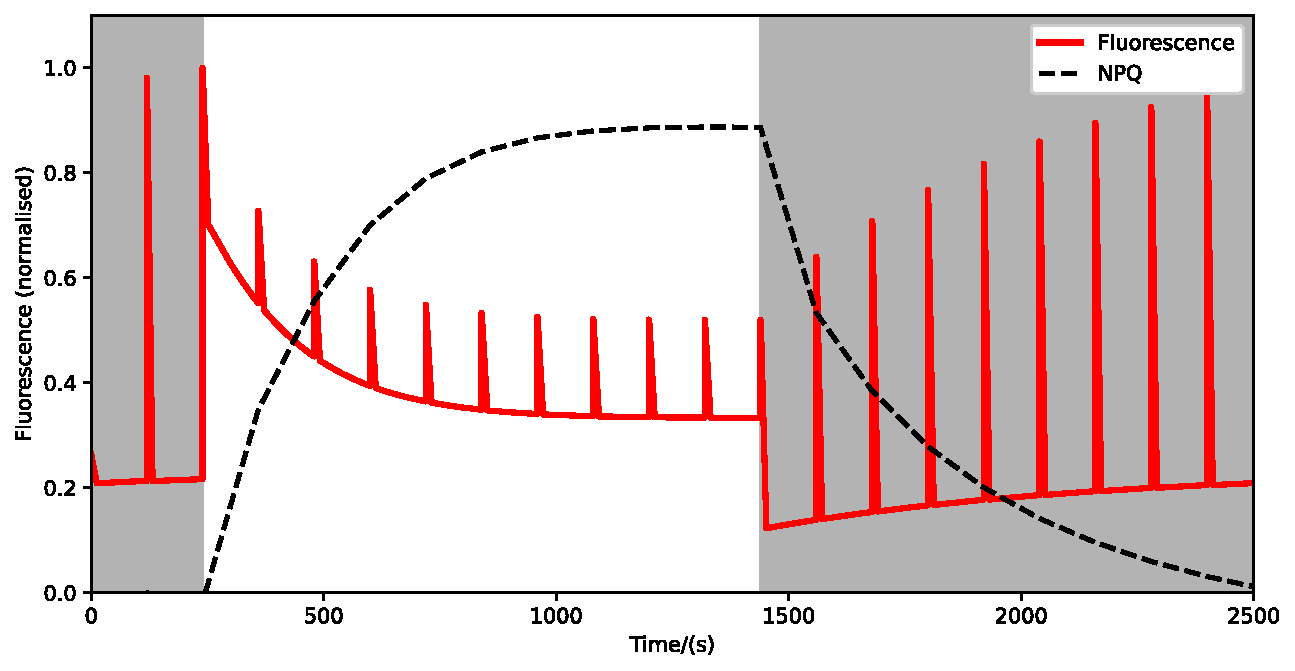
\includegraphics[width=0.7\textwidth]{Figures/Validations/saadat2021_fig2.pdf}
    \captionvalid{Saadat2021}{Results of a generic \gls{pam} protocol.}{The generic \glsentryfull{pam} protocol starts with a \qty{4}{\minute} dark period with a saturating pulse at the \qty{2}{\minute} mark. At the end of the dark period, another saturating pulse indicates the start of an actinic light period that goes on for \qty{10}{\minute}, with saturating pulses every \qty{2}{\minute}. Then another dark period of \qty{18}{\minute} starts, again with a saturating pulse at the start and at each \qty{2}{\minute} mark. The light intensity used for the actinic light period is \qty{1000}{\micro\mol\per\square\meter\per\second}, while the dark periods are \qty{40}{\micro\mol\per\square\meter\per\second}. Each saturating pulse was simulated for \qty{0.8}{\second} at a light intensity of \qty{5000}{\micro\mol\per\square\meter\per\second}. The simulation is run using the default parameters and initial conditions of the model, except for the \glsentryfull{kcyc} ($=0$) to match an organism with no cyclic electron flow. The values of light intensity were inputted directly to the \glsentryfull{ppfd} parameter of the model. The results shown are the \glsentryfull{F} which was normalized to the maximum value of that series (red), and the \glsentryfull{npq} (black), which was calculated by using the \glsentryshort{F} and \glsentryfull{Fm}~\cleverref{Eq.}{eq:npq}. This figure is recreated from figure 2 of the original publication of the Saadat2021 model~\cite{saadatComputationalAnalysisAlternative2021}.}
    \label{fig:saadat2021-fig2}
\end{figure}

\begin{figure}
    \centering
    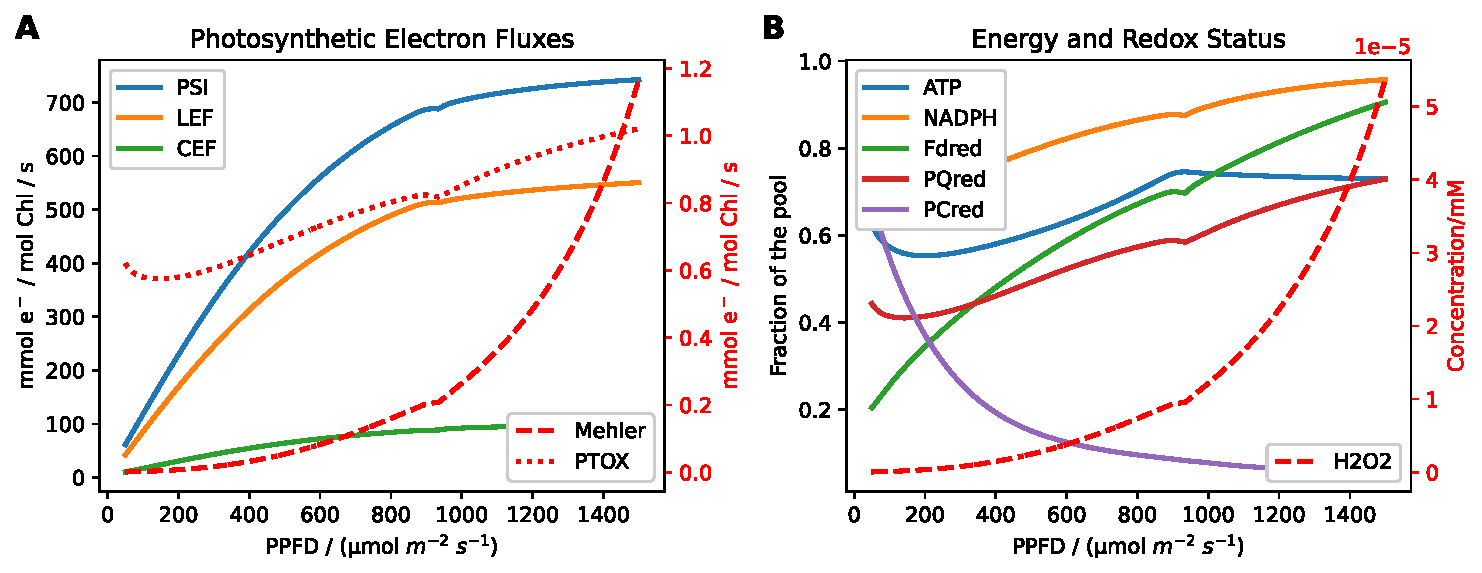
\includegraphics[width=0.7\textwidth]{Figures/Validations/saadat2021_fig3.pdf}
    \captionvalid{Saadat2021}{Results of a steady-state scan of \glsentryshort{ppfd}.}{The model was simulated to steady-state under different \glsentryfull{ppfd} values, ranging from \qty{50}{\micro\mol\per\square\meter\per\second} to \qty{1500}{\micro\mol\per\square\meter\per\second}. The results are separated in two different plots, differentiating between photosynthetic electron fluxes and the energy and redox status. The left side shows the \glsentryfull{vpsi} (blue), the \glsentryfull{lef} (orange, and calculated by doubling the \glsentryfull{vpsii}), the \glsentryfull{vcyc} (green), the \glsentryfull{vmehler} (red and dashed), and the \glsentryfull{vptox} (red and dotted). On the right side the ratios of \glsentryfull{atp} (blue), \glsentryfull{nadph}  (orange), \glsentryfull{fdred} (green), \glsentryfull{pqred} (red), and \glsentryfull{pcred} (purple) to their total pools are shown. Additionally the concentration of \glsentryfull{h2o2} (red, dashed) is also plotted. The simulation is run using the default parameters and initial conditions of the model, while changing only the \glsentryfull{ppfd} to the desired value for each simulation. This figure is recreated from figure 3 of the original publication of the Saadat2021 model~\cite{saadatComputationalAnalysisAlternative2021}.
    }
    \label{fig:saadat2021-fig3}
\end{figure}

\begin{figure}
    \centering
    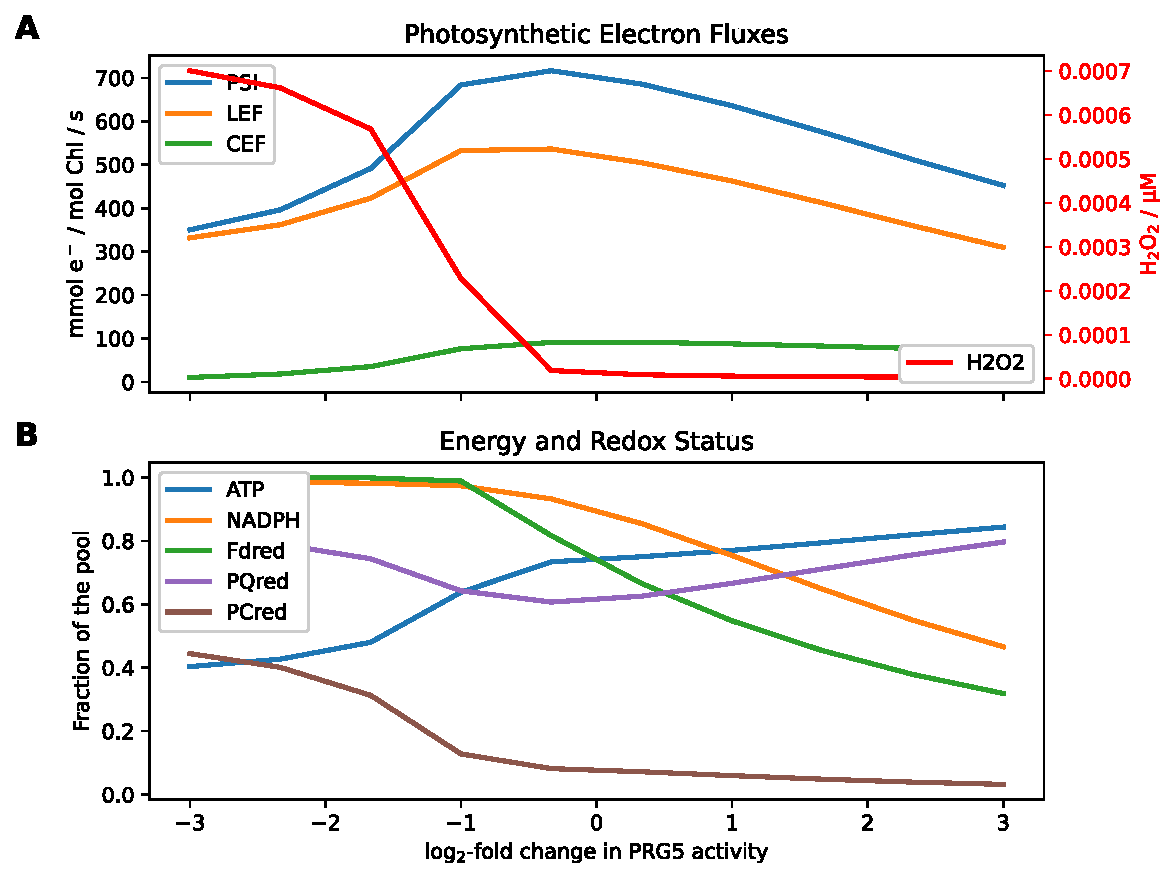
\includegraphics[width=0.7\textwidth]{Figures/Validations/saadat2021_fig4.pdf}
    \captionvalid{Saadat2021}{Results of a steady-state scan of aletered \glsentryshort{cef}.}{The model was simulated to steady-state under different \glsentryfull{kcyc} values representing $\log_2$-fold changes ranging from negative three to three. The results are separated in two different plots, differentiating between photosynthetic electron fluxes and the energy and redox status. The top plot shows the \glsentryfull{vpsi} (blue), the \glsentryfull{lef} (orange, and calculated by doubling the \glsentryfull{vpsii}), the \glsentryfull{vcyc} (green), and the concentration of \glsentryfull{h2o2} (red). In the bottom plot the ratios of \glsentryfull{atp} (blue), \glsentryfull{nadph}  (orange), \glsentryfull{fdred} (green), \glsentryfull{pqred} (red), and \glsentryfull{pcred} (purple) to their total pools are shown. The simulation is run at a \glsentryfull{ppfd} of \qty{1000}{\micro\mol\per\square\meter\per\second}, otherwise using the default parameters and initial conditions of the model, while changing only the \glsentryshort{kcyc} to the desired value for each simulation. Due to issues of singular ranges of \glsentryshort{kcyc} not being able to be simulated to steady-state, only a few values could actually be plotted, to bee seen by the jaggedness of the lines. This figure is recreated from figure 3 of the original publication of the Saadat2021 model~\cite{saadatComputationalAnalysisAlternative2021}.}
    \label{fig:saadat2021-fig4}
\end{figure}

\begin{figure}
    \centering
    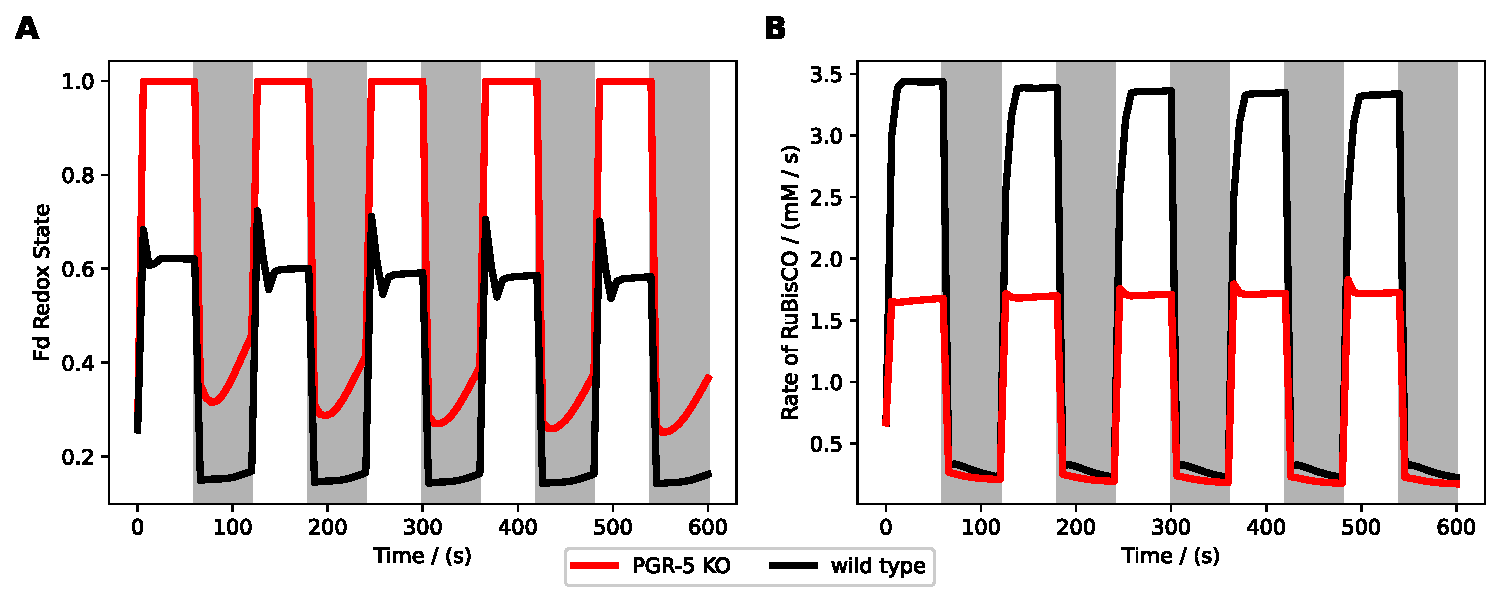
\includegraphics[width=0.7\textwidth]{Figures/Validations/saadat2021_fig5.pdf}
    \captionvalid{Saadat2021}{Comparison of results of a wildtype and knockout mutant simulation under varying light intensities.}{A simple fluctuating light protocol was used to simulate a wildtype (black) and a knockout mutant (red) of the model. The protocol undergoes a total of 10 periods, each of them lasting \qty{1}{\minute}. The light intensities of the periods alternate between light and dark, using a light intensity of \qty{600}{\micro\mol\per\square\meter\per\second} and \qty{40}{\micro\mol\per\square\meter\per\second}, respectively. The wildtype simulation was run using the default parameters and initial conditions of the model, while the knockout mutant was simulated by setting the \glsentryfull{kcyc} to zero. Each light intensity was inputted into the \glsentryfull{ppfd} parameter of the models. The results shown are the ratio of \glsentryfull{fdred} to its total pool on the left, and the \glsentryfull{vc} on the right. This figure is recreated from figure 5 of the original publication of the Saadat2021 model~\cite{saadatComputationalAnalysisAlternative2021}.}
    \label{fig:saadat2021-fig5}
\end{figure}

\begin{figure}
    \centering
    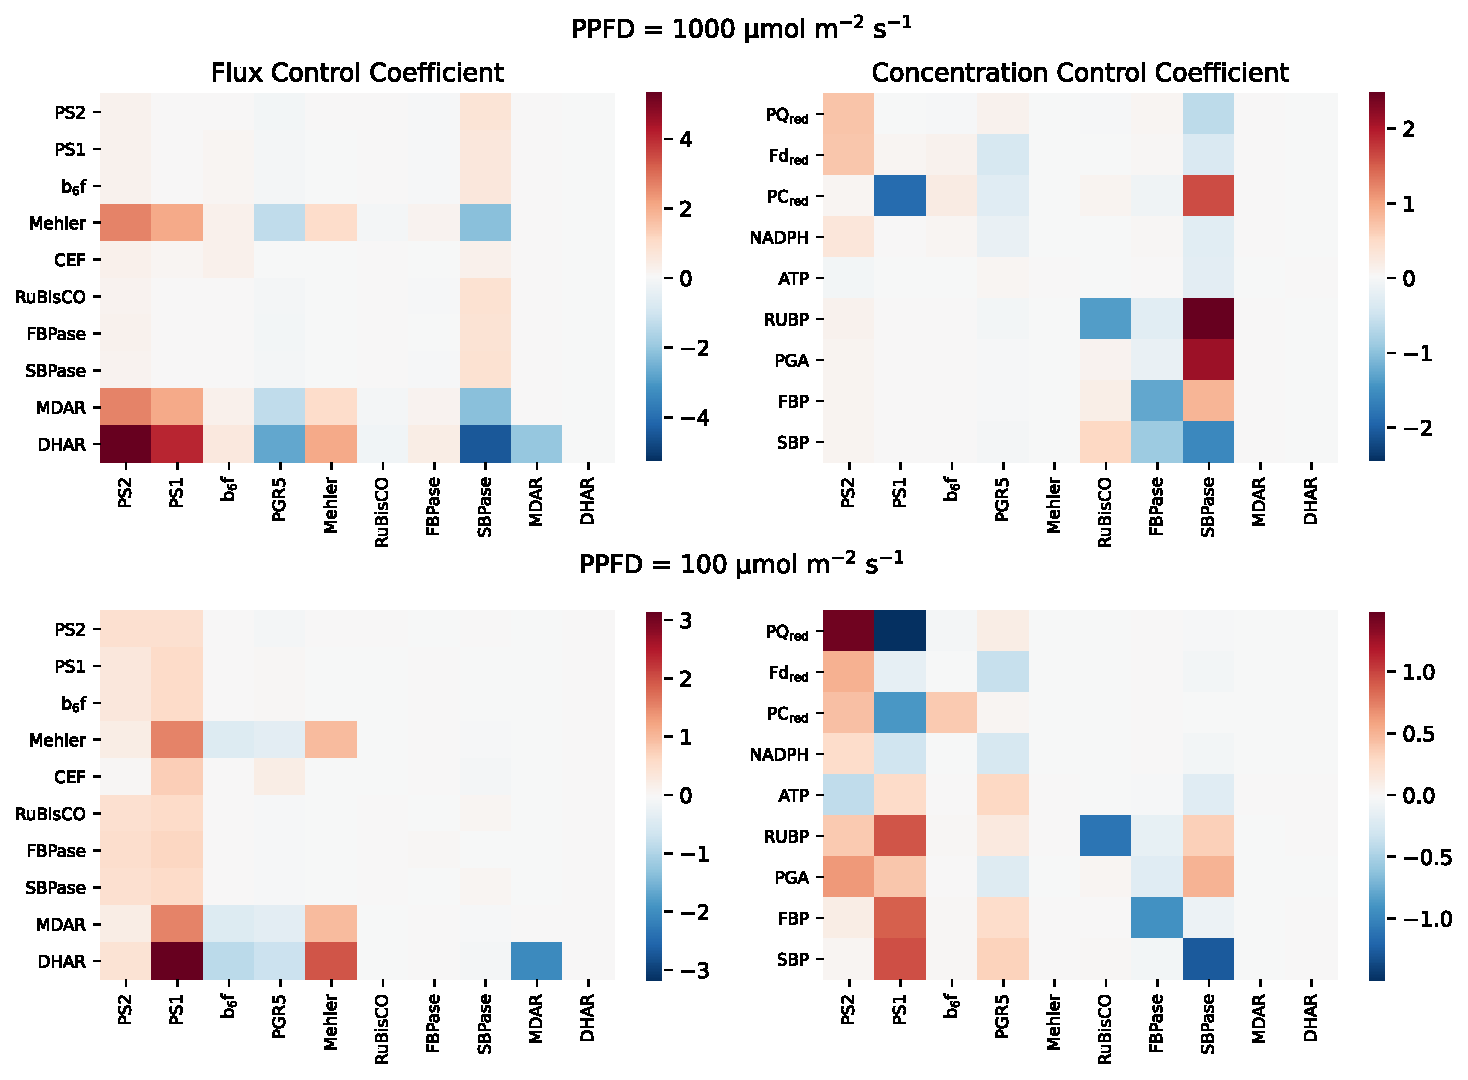
\includegraphics[width=0.7\textwidth]{Figures/Validations/saadat2021_fig6.pdf}
    \captionvalid{Saadat2021}{\glsentryshort{mca} of key aspects of the model under two different light intensities.}{A \glsentryfull{mca} was done to the model under two different light intensities, \qty{1000}{\micro\mol\per\square\meter\per\second} (top) and \qty{1000}{\micro\mol\per\square\meter\per\second} (bottom). The results of the fluxes can be found on the left, while on the right are the variables. The parameters that were used for the \glsentryshort{mca} are the control coefficients of the fluxes with the same names. The following were used, given from left to right on the x-axis of each heatmap: \glsentryfull{psiitot}, \glsentryfull{psitot}, \glsentryfull{kcatb6f}, \glsentryfull{kcyc}, \glsentryfull{kmehler}, \glsentryfull{kcatvc}, \glsentryfull{kcatfbpase}, \glsentryfull{kcatsbpase}, \glsentryfull{kcatmdareduct}, and \glsentryfull{kcatdhar}. These parameters were displaced by $\pm 1\%$. The simulations were otherwise done using the default parameters and initial conditions of the model, while changing only the \glsentryfull{ppfd} to the desired value for each simulation. This figure is recreated from figure 6 of the original publication of the Saadat2021 model~\cite{saadatComputationalAnalysisAlternative2021}.
    }
    \label{fig:saadat2021-fig6}
\end{figure}

The last figure of the publication includes the same parameter range as the fourth figure, therefore the same issue is observed in the recreation. However in this case, the recreation could not be completed at all, as the specific range of the \gls{kcyc} parameter where these oscillations are found is not well documented.

\subsection{Model Demonstrations}

\subsubsection{Daylight Simulation}

The light intensity during the chosen day period follows an approximate bell curve, common for these sorts of graphs. As sunlight is not a constant source, but may change dynamically due to weather conditions, the light intensity shows simple peaks and valleys during the entire day. This allows to test the capabilities of the models to simulate complex and dynamic light protocols, which is a common issue for many models. In this case, all but the Li2021 model show results to varying degree~\figref{fig:daylight-demon}.

The Bellasio2019 model shows a clear response to the changing light conditions, both the \gls{vc} and the \gls{atp} and \gls{nadph} ratio rising and falling with the light intensity during the day. However, at approximately 10:30, both reach a plateau, that goes on until approximately 16:00, where the light intensity begins to fall. There the \gls{vc} slowly begins to fall to 0 until the end of the simulation, while the \gls{atp} and \gls{nadph} ratio slowly rises until 18:00 and then falls following the pattern of the \gls{vc} line. As this model does not have a quantity representing \gls{F}, it cannot be plotted.

The Fuente2024 model only has a representative quantity for \gls{F}, which follows the light intensity pattern very closely. However, in the moments of lower light, the \gls{F} values are more sensitive to the light fluctuations, as for example the peak at 08:00 causes the \gls{F} to rise to the same values as during the highest light intensities. Additionally, the \gls{F} values show a small rise when the day begins to end, which does not follow the light intensity pattern. However, in the higher light intensities, the \gls{F} values do follow the light intensity pattern very closely.

The Matuszynska2016 model, also only shows a representative quantity for \gls{F}, which also follows the light intensity pattern very closely. Just like with the Fuente2024 model, the \gls{F} values follow the light pattern closest during the higher light intensities, while during the lower light intensities, they are more sensitive to the light fluctuations. Interestingly, this model also shows a small rise in \gls{F} values when the day begins to end.

The Saadat2021 model shows all three representative quantities, \gls{vc}, \gls{atp} and \gls{nadph} ratio, and \gls{F}. The \gls{vc} values show a clear correlative response to the light intensity, rising and falling with the light intensity during the day. Comparatively to the Bellasio2019 model, these values also reach a plateau at 10:30 and slowly fall after 16:00. Contrary to the other models though, both the \gls{atp} and \gls{nadph} ratio, and the \gls{F} values show an anticorrelative response to the light intensities. Especially the \gls{F} which drops significantly during the higher light intensities, while rising during the lower light intensities. It also reaches a plateau at 10:30, but then slowly rises at 16:00, to reach approximately the same starting value as of the start of the day. The \gls{atp} and \gls{nadph} ratio also shows a similar pattern, but with less significant changes.

\begin{figure}
    \centering
    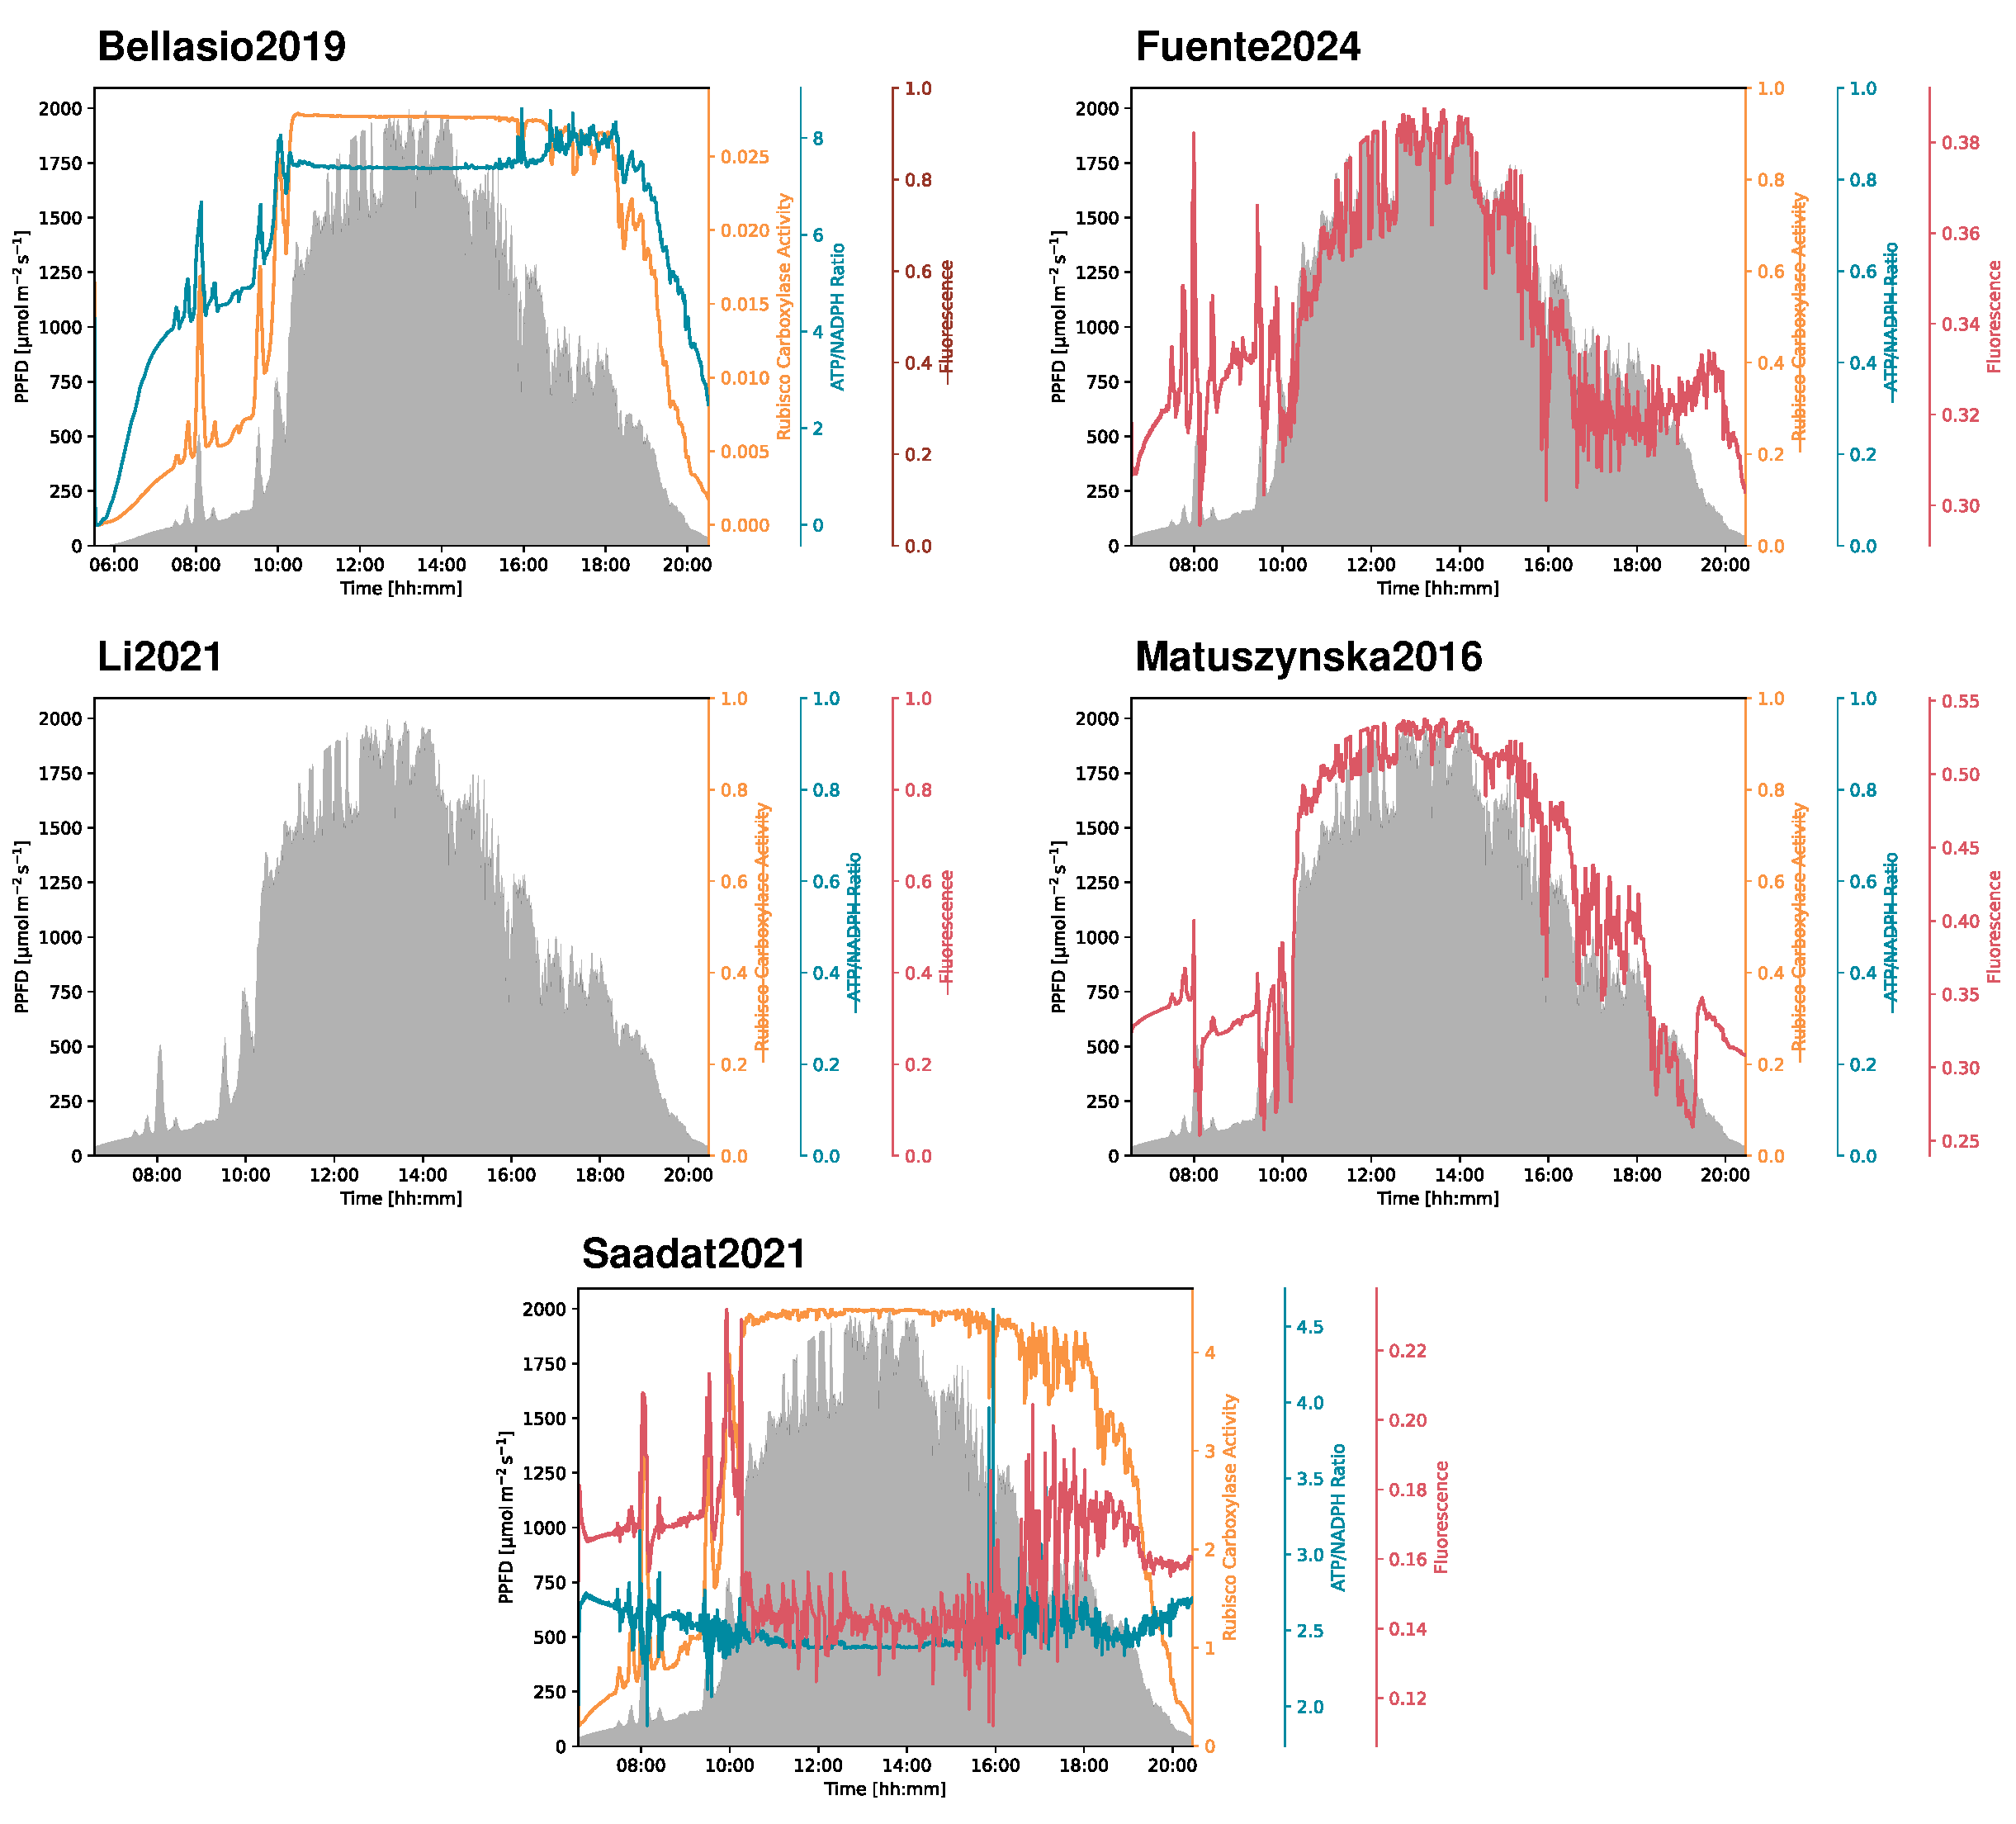
\includegraphics[width=0.7\textwidth]{Figures/Demonstrations/daysimulation.pdf}
    \captionprof{Combined Daylight Simulation demonstrations of all models.}{Sample simulation of a day cycle using real \glsentryfull{ppfd} data from Kansas, USA on June 19, 2023. The data was obtained from the \glsentryfull{neon} data portal~\cite{nationalecologicalobservatorynetworkneonPhotosyntheticallyActiveRadiation2023} and is used to create a protocol for the light intensity \glsentryshort{ppfd} over the course of the day, in a minute interval. The data used is filtered to only show a \glsentryshort{ppfd} that equals or is higher than \qty{40}{\micro\mol\per\square\meter\per\second}. This threshold is chosen as it has shown to allow most models to still simulate the photosynthetic machinery, while still being a decent representation of the actual daylight conditions. The simulation is run using the default parameters and initial conditions of each model, and the \glsentryfull{vc}, \glsentryfull{atp} and \glsentryfull{nadph} ratio, and \glsentryfull{F} results is plotted over the course of the day, if possible. The results do not represent actual plant behavior, but show the capabilities of the model to simulate complex and more realistic light protocols.} 
    \label{fig:daylight-demon}
\end{figure}

\subsubsection{FvCB Add-on}

Only the Bellasio2019 and Saadat2021 models have a successful demonstration of the \gls{fvcb} add-on, as the other models do not have the required quantities'~\figref{fig:fvcb-demon}. The Fuente2024, Li2021 and Matuszynska2016 models all do not include a representation for \gls{vc} and \gls{co2}. Without these, a \gls{fvcb} style assimilation could not be calculated.

The Bellasio2019 on the other hand, shows a very distinct correlation between the simulation results and the min-W \gls{fvcb} model, with general parameters used~\cite{lochockiWidelyUsedVariants2025a}. However, once the simulation is done at higher \gls{ci} values, both the \gls{vc} and \gls{A} values drop below the \gls{fvcb} model. On top of that, they are small divots in the simulation results, which may be resulted in an unsuccessful steady-state analysis, and therefore an automatic rescue to a quasi-steady-state, \qty{1800}{s}, was performed.

The Saadat2021 model results have approximately the same shape of curve than the \gls{fvcb} model, but the ascent is much steeper. This can be seen, by the \gls{A} of the Saadat2021 model beginning lower but ending higher than the \gls{fvcb} \gls{A}. Both of the \gls{vc} start at the same point, namely \qty{0}{\micro\mol\per\meter\squared\per\second}, but the Saadat2021 model also reaches a higher value.

\begin{figure}
    \centering
    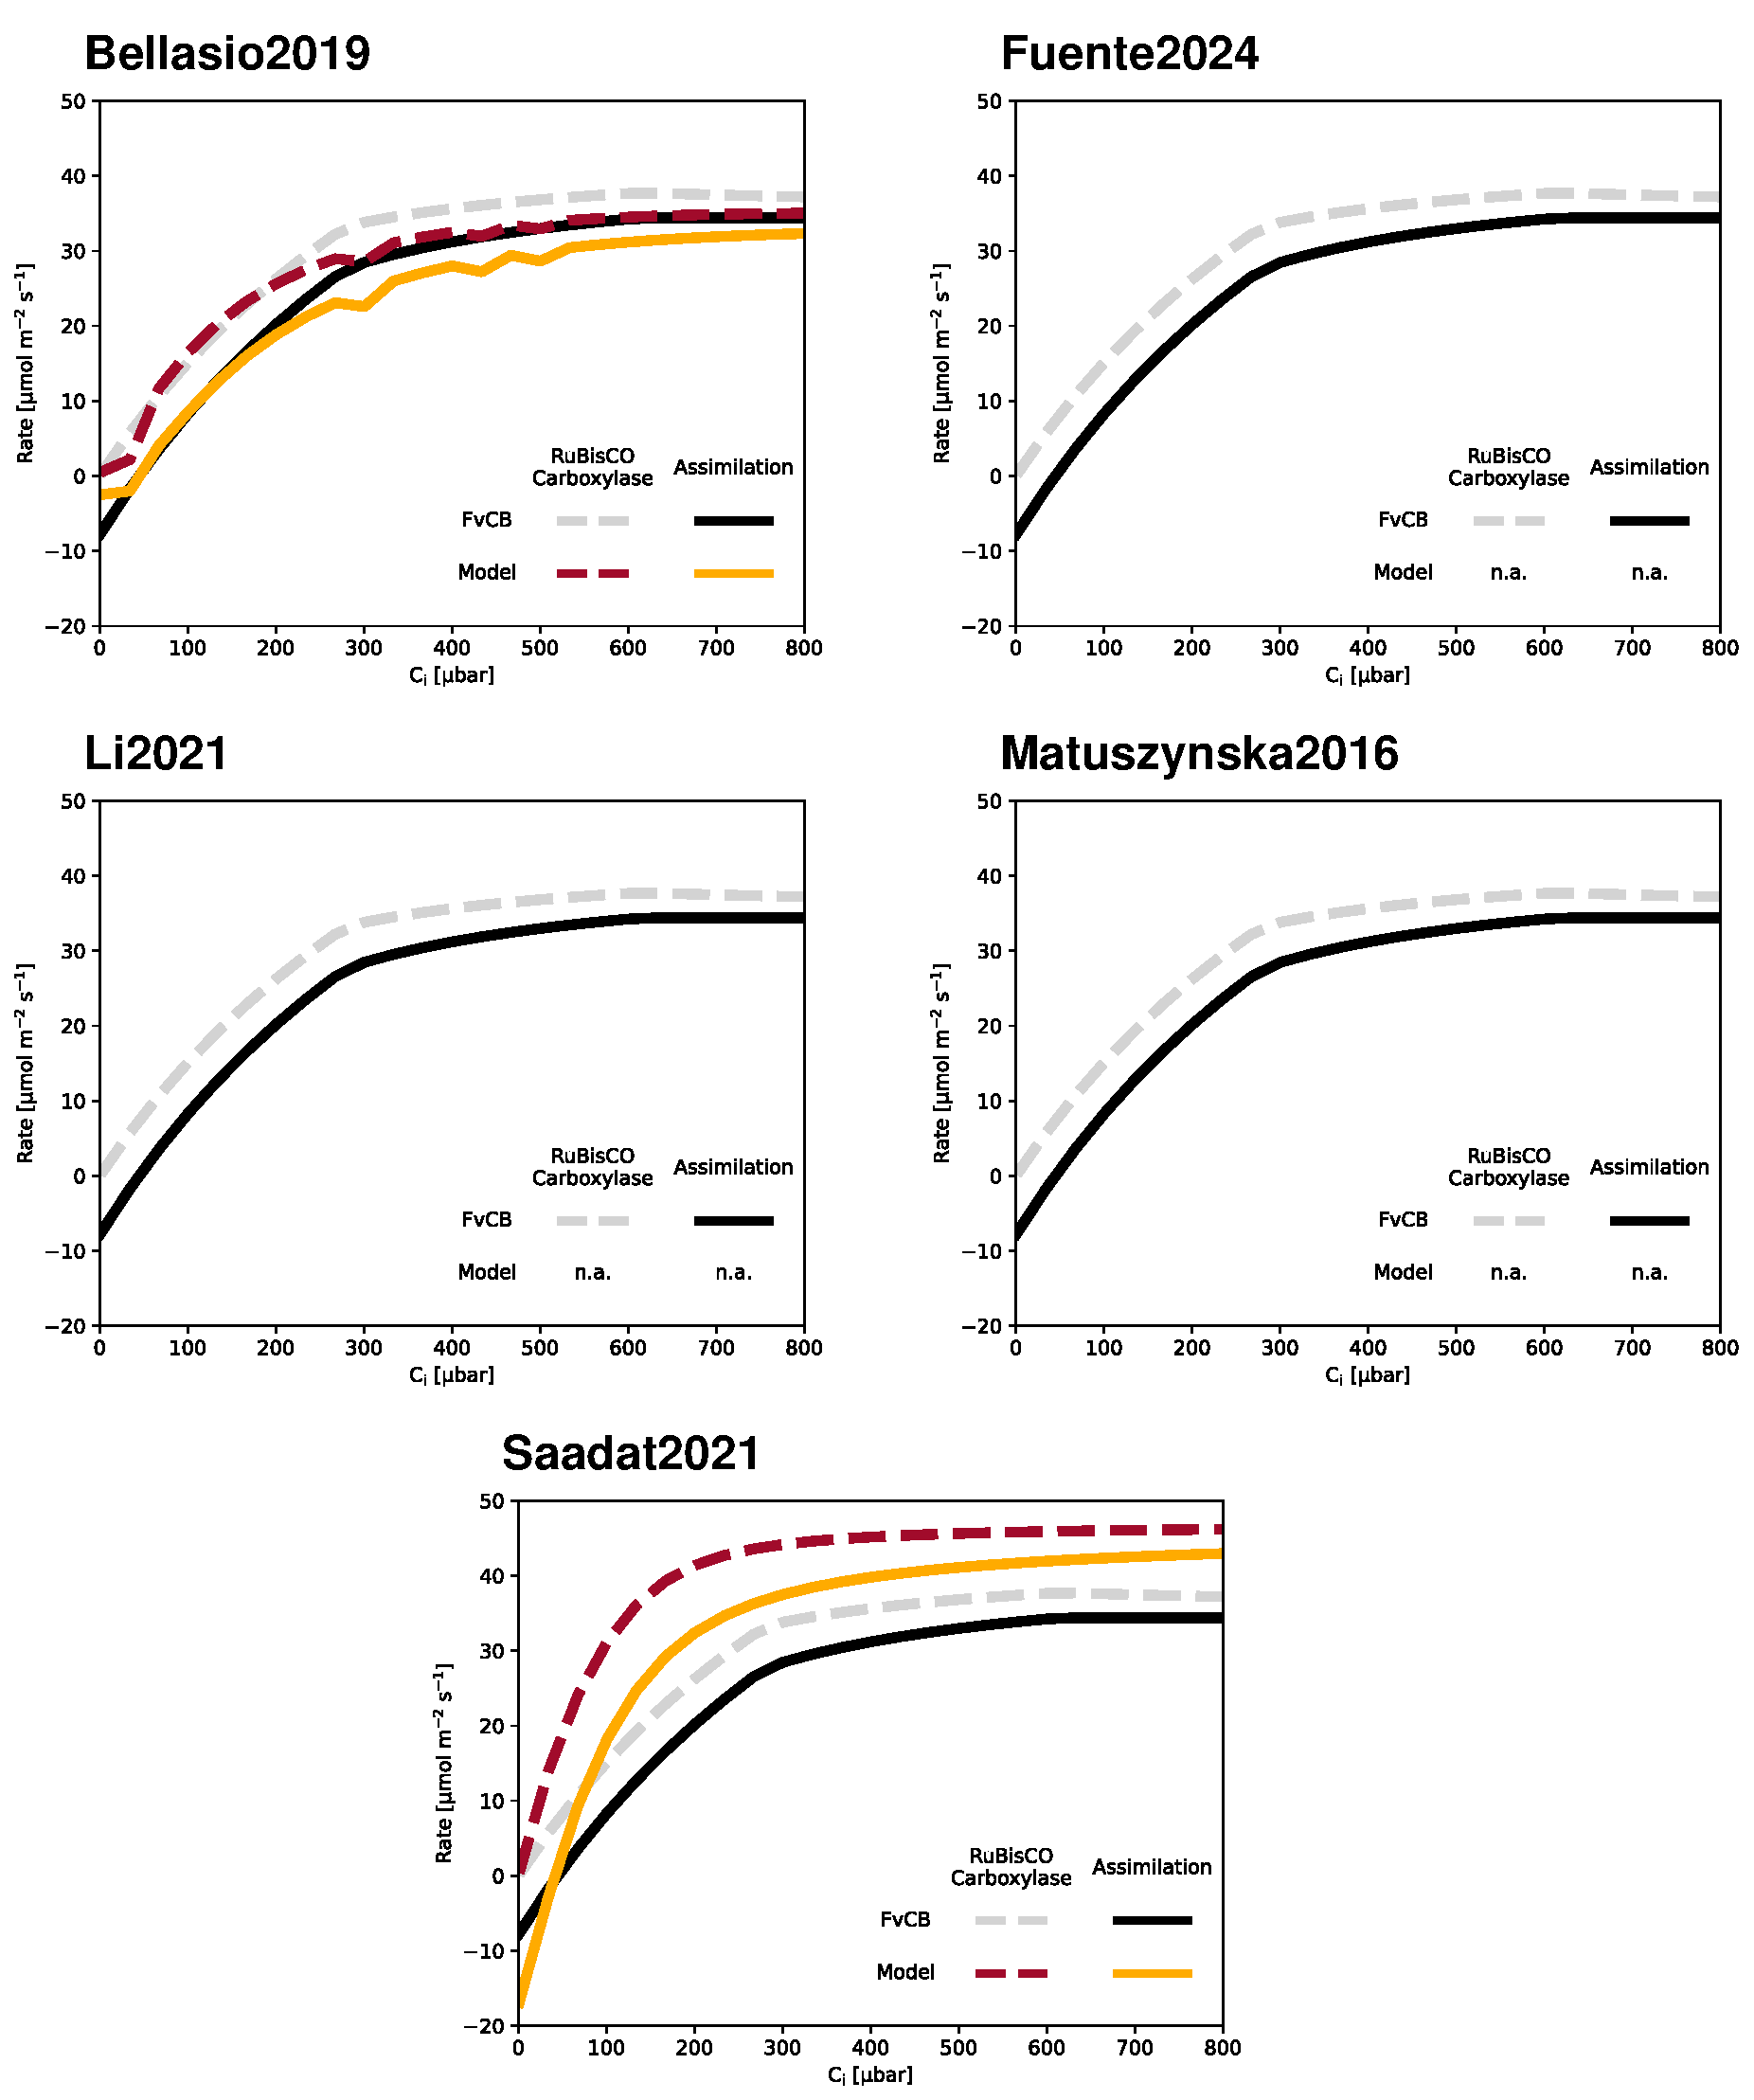
\includegraphics[width=0.7\textwidth]{Figures/Demonstrations/fvcb.pdf}
    \captionprof{Combined FvCB Addon demonstrations of all models.}{Comparison of modelled \glsentryfull{A} and \glsentryfull{vc} against the \glsentryfull{fvcb} model. The \glsentryshort{fvcb} model is calculated using the min-W approach as described by Lochoki and McGrath (2025)~\cite{lochockiWidelyUsedVariants2025a}. To be able to simulate \glsentryshort{A}, there are two mandatory quantities that need to be present in the model: \glsentryfull{co2} concentration and \glsentryshort{vc}. If one of these parameters is missing, the \glsentryshort{fvcb} model will still be shown, but no comparison with the model will be possible. Other parameters that are required to calculate the \glsentryshort{fvcb} model will be added as parameters with default values if they are not present in the model. The simulation is then run until steady-state, or quasi-steady-state if not otherwise possible, for different \glsentryfull{ci} partial pressure. The carbon assimilation shown does not represent actual values but rather a theoretical curve to compare the kinetic model to the popular \glsentryshort{fvcb} model.} 
    \label{fig:fvcb-demon}
\end{figure}

\subsubsection{Standard PAM Simulation}

All models show a successful demonstration of the standard \gls{pam} simulation~\figref{fig:pam-demon}, except the Bellasio2019 model, which does not have a quantity representing \gls{F} nor \gls{npq}. Additionally, the Li2021 model only includes a quantity for \gls{npq}, which shows a typical curve of \gls{npq} for the standard protocol. However, at the start of the protocol, an uncommon small peak can be seen, with a slow ascent and descent. Due to the fact, that the model does not contain a quantity for \gls{F}, it is harder to see the different points of time when a saturating pulse was used. Still, due to the continuous simulation of the \gls{npq}, the curve is much smoother than the other models, and small spikes can be seen that can be attributed to time points of saturating pulses.

The Fuente2024, Matuszynska2016, and Saadat2021 models all follow the typical pattern for \gls{F} a \gls{pam} protocol. The \gls{F} values starting relatively high after the dark adaptation period, with the \gls{Fm} at saturating pulses being the highest in the first dark period. Then the base \gls{F} values stay stagnant during the actinic light period, where they are higher than during the prior dark period for the Fuente2024 and Matuszynska2016 models, but lower for the Saadat2021 model. In the same light period, the \gls{Fm} values quickly drop to a lower and stable value in all three models. Then during the second dark period for all three models, the base \gls{F} values drop even lower than in the first dark period, but slowly rising back following the simulation time. The \gls{Fm} values all gradually rise during the second dark period, but do not reach the same values as during the first period.

The \gls{npq} curves of all three models also follow a typical pattern, with them start at near 0 in the first dark period, then quickly rising to a stable value in a curve during the actinic light period. Only the Saadat2021 model, shows a \gls{npq} curve in the actinic light period that reaches over its stagnating point at the start. However, then all three models show a curved drop during the second dark period, reaching a stable value that is higher than at the starting point. As the Matuszynska2016 and Saadat2021 models do not have a quantity for \gls{npq}, it had to be calculated using \gls{F} and \gls{Fm}~\cleverref[]{Equation}{eq:npq}, meaning the amount of points for the \gls{npq} curves is the same as the number of \gls{Fm} present in the simulation. This creates a more jagged curve, while the Fuente2024 model, which has a quantity for \gls{npq}, shows a smoother curve.

\begin{figure}
    \centering
    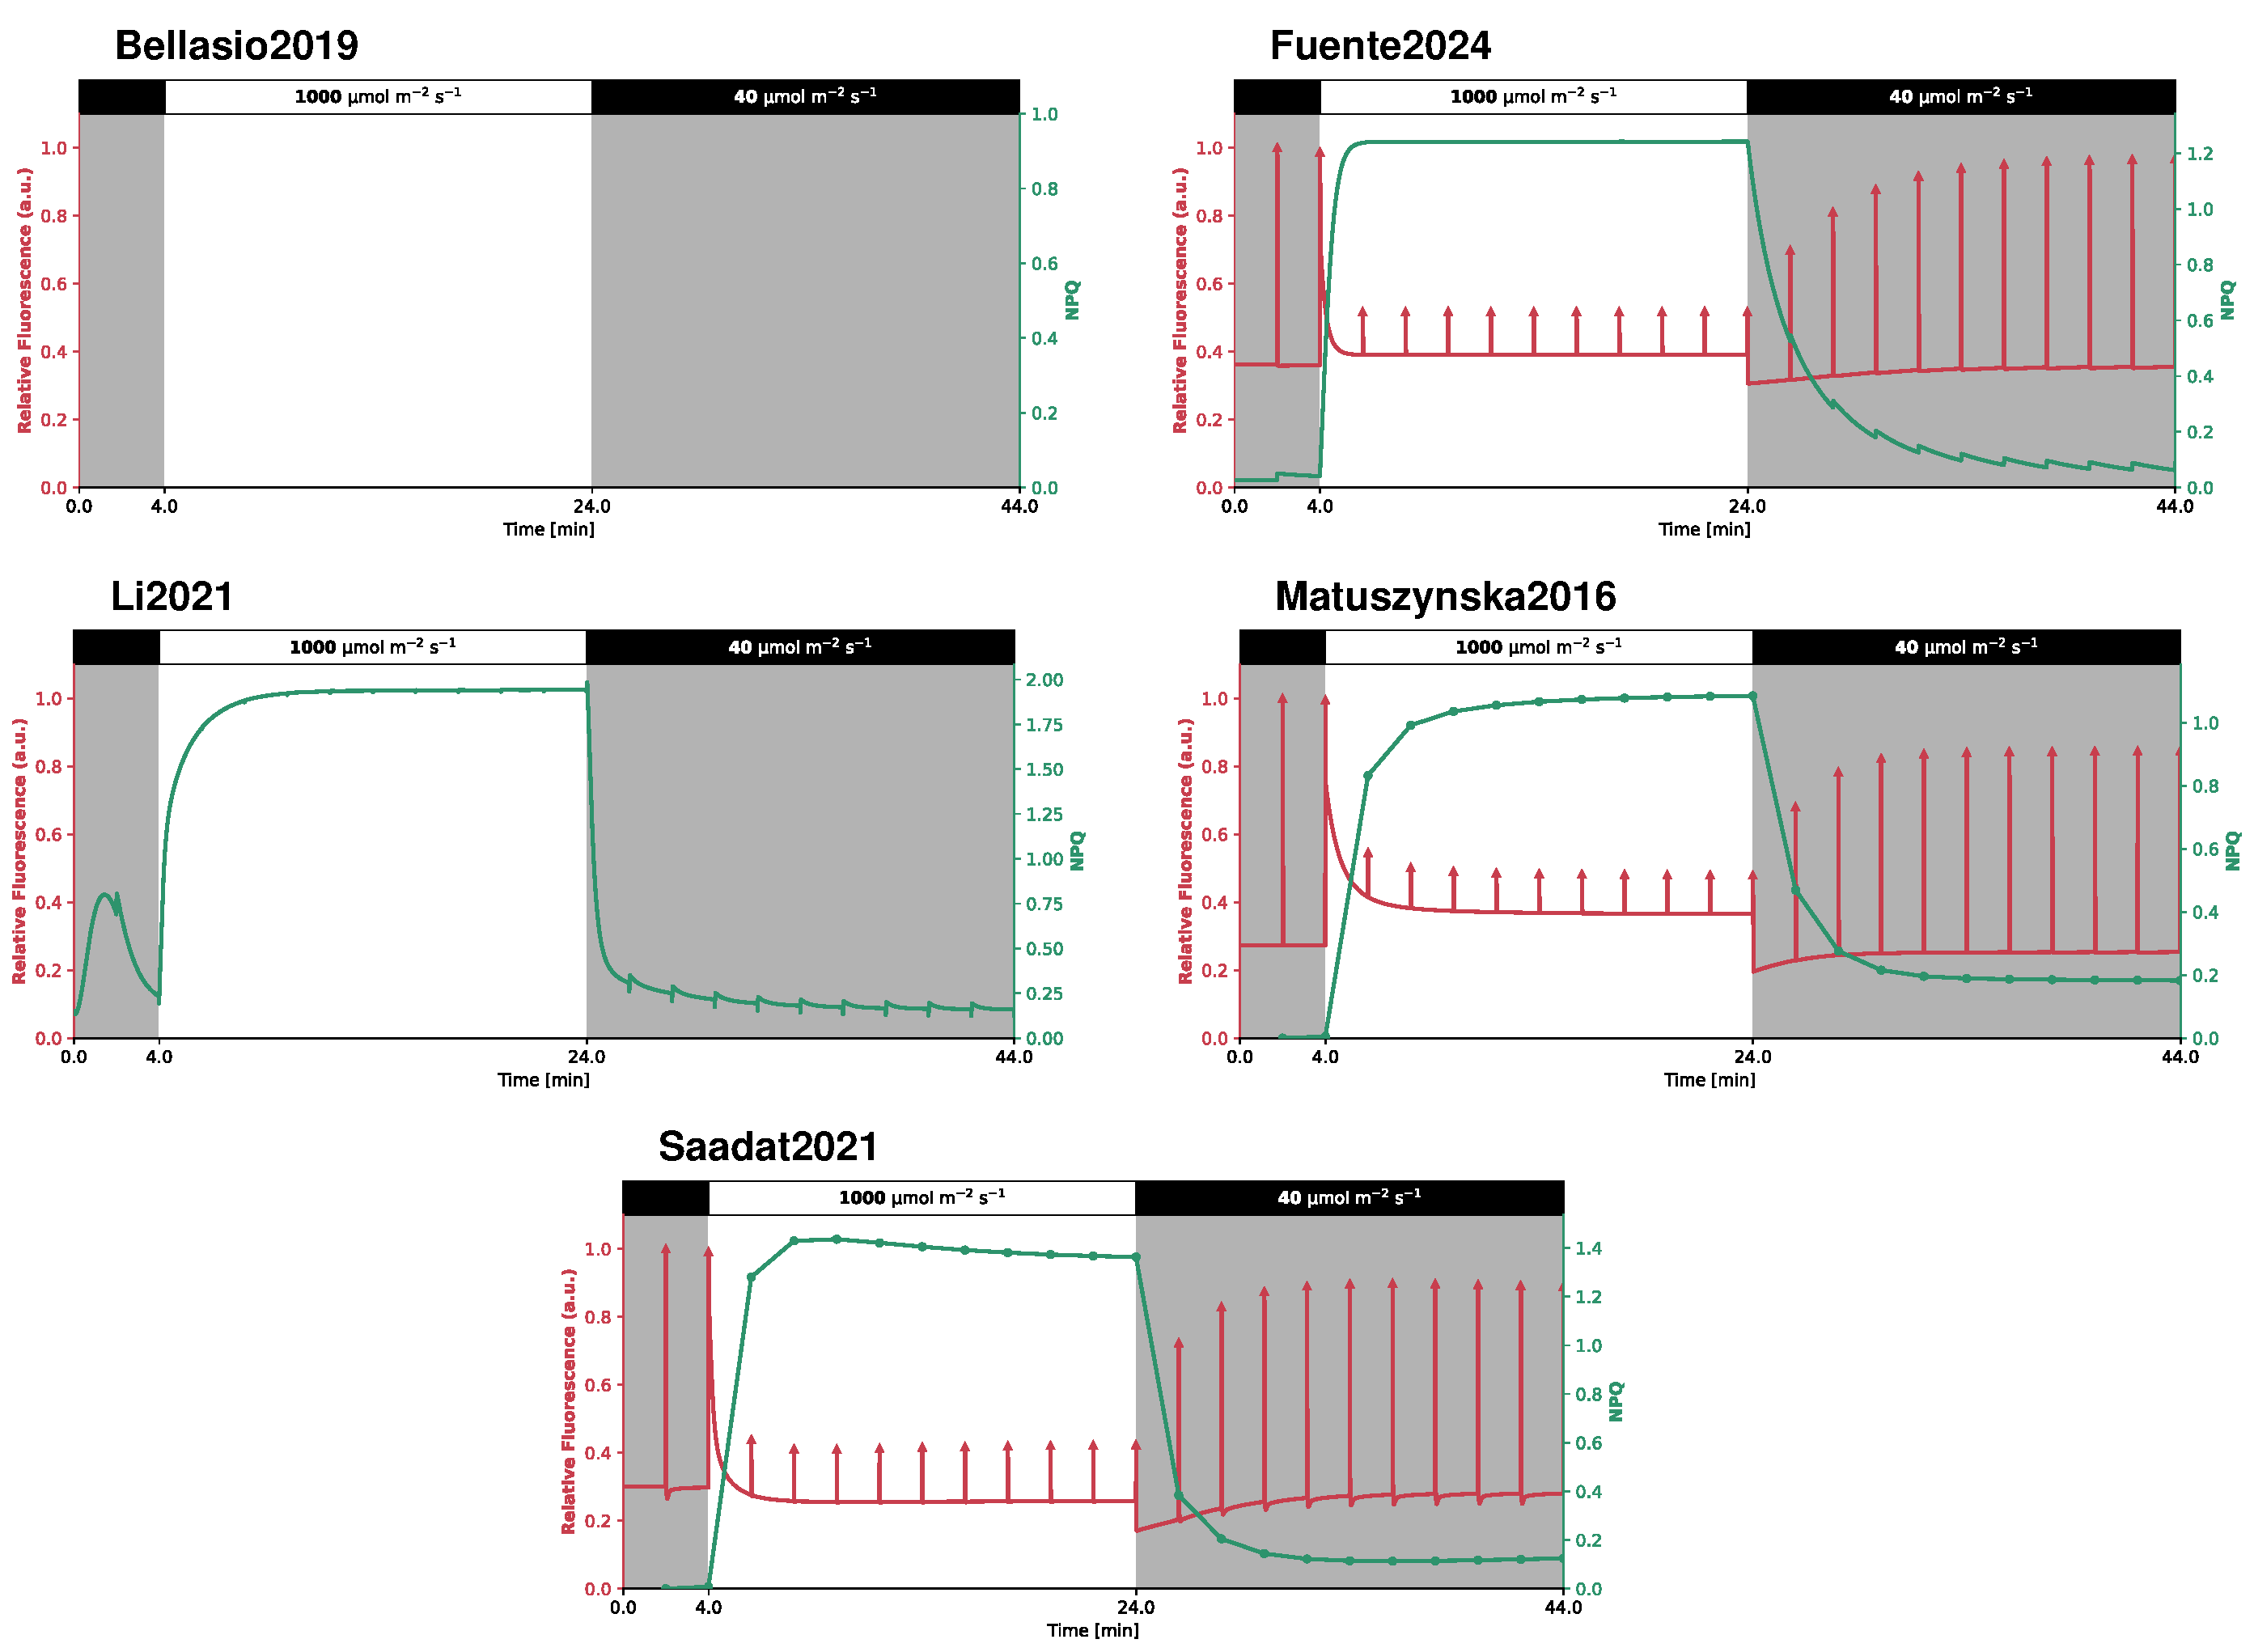
\includegraphics[width=0.7\textwidth]{Figures/Demonstrations/pam.pdf}
    \captionprof{Combined PAM Simulation demonstrations of all models.}{Sample simulation of a common \glsentryfull{pam} protocol to show fluctuations of \glsentryfull{F} and \glsentryfull{npq} using saturating pulses. The simulation protocol is as follows: A dark adaptation period that simulates for 30 minutes at a dark light intensity (\qty{40}{\micro\mol\per\square\meter\per\second}), then the actual protocol starts. The protocol consists of 22 periods with each being 2 minutes of length. That period consists of a specific light intensity of the respective type of period and ends with a saturating pulse with a length of \qty{0.8}{s} and a light intensity of \qty{3000}{\micro\mol\per\square\meter\per\second}. First, two dark periods with light intensity of \qty{40}{\micro\mol\per\square\meter\per\second}, followed by ten light periods with light intensity of \qty{1000}{\micro\mol\per\square\meter\per\second}, then ten dark periods again. The simulation is run using the default parameters and initial conditions of each model.}
    \label{fig:pam-demon}
\end{figure}

\subsubsection{MCA of Photosynthesis}

No models could complete the entire \gls{mca} heatmaps, neither the variables nor the fluxes~\figref{fig:mca-demon}. On top of that, the Li2021 shows completely empty heatmaps, even though it has some of the required quantities to perform the \gls{mca}. This is due to the model not being able to achieve steady-state for the parameters scanned, which is required for a \gls{mca} analysis on control coefficients.

The Bellasio2019 model shows results for the control coefficients of \gls{psii} and \gls{rubisco} for \gls{rubp}, \gls{co2}, \gls{atp}, and \gls{nadph} for the variables, and \gls{vc}, and \gls{vatp} for the fluxes. Both control coefficients do not have much control on the variables, except for the \gls{rubisco} coefficient on \gls{rubp}, which shows a strong negative control. On the fluxes side, both coefficients do not show much control on both \gls{vc} and \gls{vatp}.

The Fuente2024 model only shows results for the control coefficients of \gls{psii} and \gls{psi} for \gls{pq_ox}, \gls{atp}, \gls{vpsi}, and \gls{vpsii}. The control coefficient of \gls{psii} does not have much on either the variables or the fluxes mentioned prior. The control coefficient of \gls{psi} shows a strong positive control on \gls{pq_ox} and \gls{vpsi}, but also a smaller positive control on \gls{atp} and \gls{vpsii}.

The coefficients that are included in the Matuszynska2016 model are representative of \gls{psii}, \gls{cytb6f} and \gls{atp} synthase. The only viable variable in this model is \gls{atp}, which is positively controlled by all three coefficients, but most strongly by the coefficient of \gls{psii}. The fluxes that are included in this model are \gls{vpsii}, \gls{vb6f}, and \gls{vatp}. All the coefficients have a positive control on all the fluxes and show a consistent pattern respective to each coefficient, with the coefficient of \gls{psii} also having the strongest control on all three fluxes.

The Saadat2021 model includes the most control coefficients of the photosynthesis \gls{mca} out of all the models. It includes the coefficients of \gls{psii}, \gls{rubisco}, \gls{cytb6f}, and \gls{atp} synthase. Nearly all coefficients have only a small control on the variables and fluxes. Except the coefficient of \gls{cytb6f}, which has a low negative control on \gls{pc_ox} and the coefficient of \gls{rubisco} which has a stronger negative control, but on \gls{rubp}. On the fluxes side, only the coefficient of \gls{psii} shows a significant positive control on all the fluxes. The other coefficients do not show any control.

\begin{figure}
    \centering
    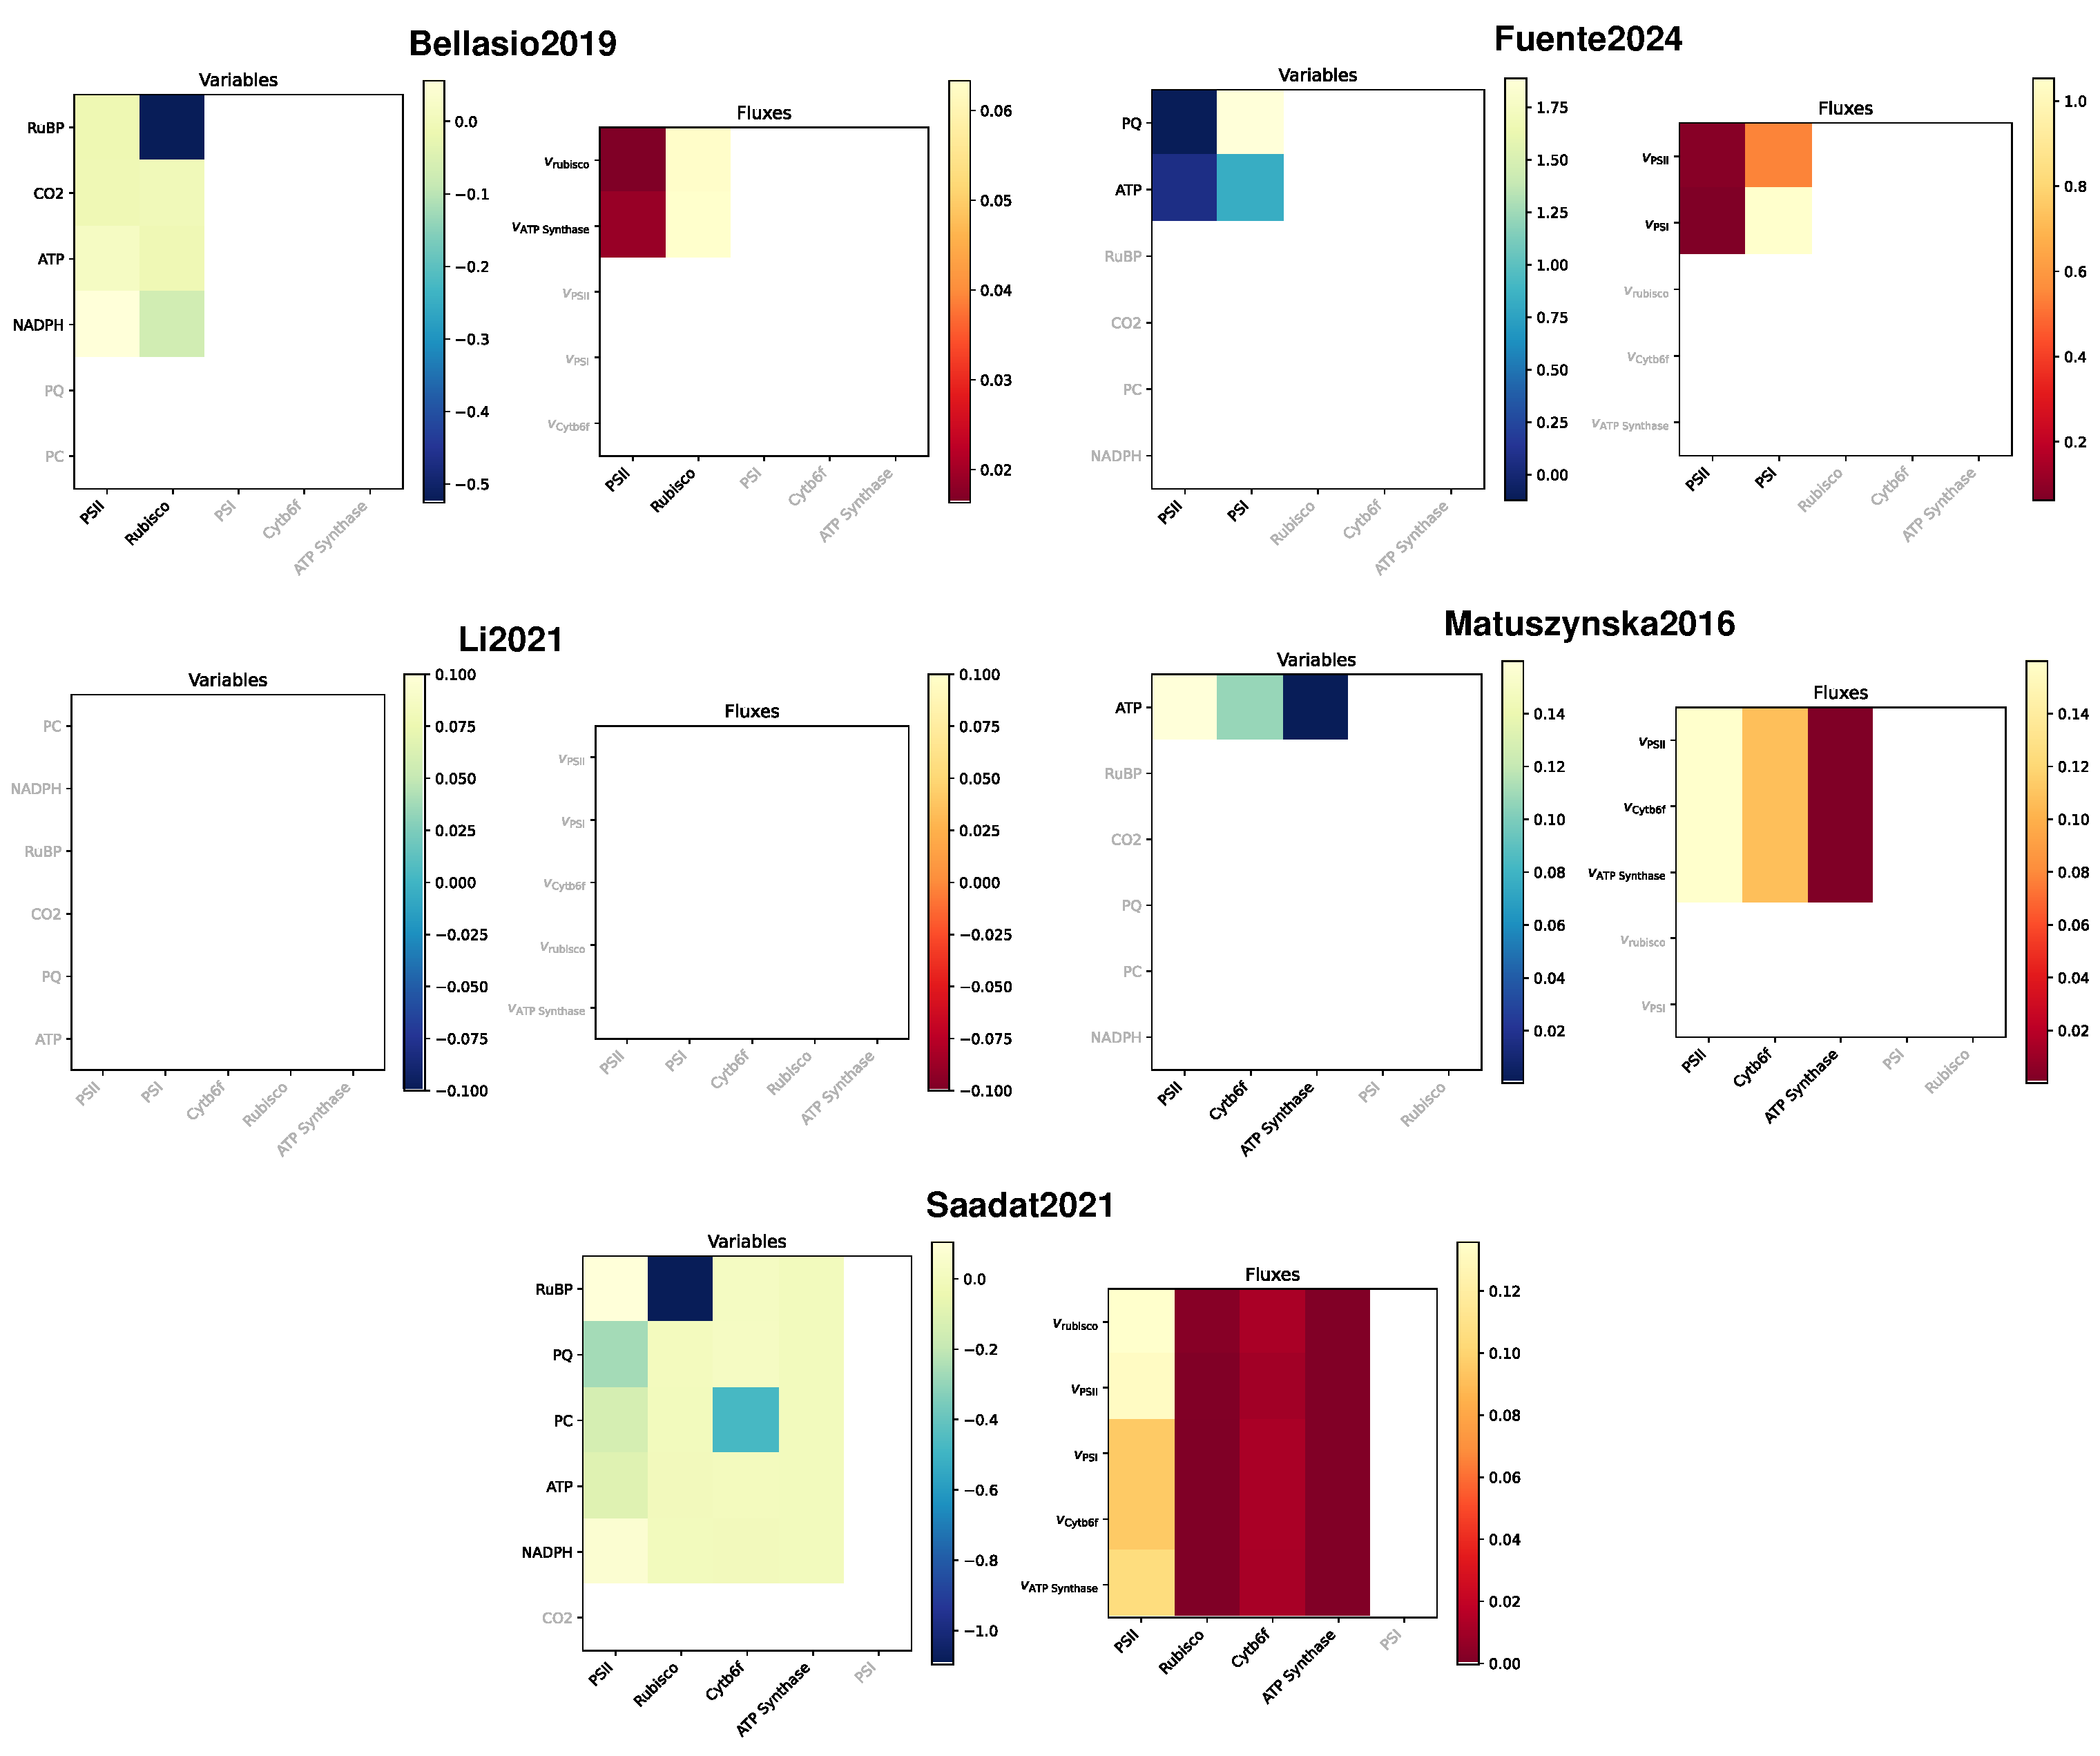
\includegraphics[width=0.7\textwidth]{Figures/Demonstrations/mca.pdf}
    \captionprof{Combined MCA of Photosynthesis demonstrations of all models.}{A sample \glsentryfull{mca} of typical photosynthesis variables and fluxes. A control coefficient analysis is to be performed, therefore each parameter represents a single coefficient of the photosynthesis rate. The rates chosen should represent \glsentryfull{vc}, \glsentryfull{vpsii}, \glsentryfull{vpsi}, \glsentryfull{vb6f} and \glsentryfull{vatp}. The variables chosen should represent \glsentryfull{co2} concentration, \glsentryfull{rubp}, \glsentryfull{pq_ox}, \glsentryfull{pc_ox}, \glsentryfull{atp}, and \glsentryfull{nadph}. For each parameter to be scanned, the model is simulated to steady-state, with a displacement of $\pm 0.01\%$ of each respective parameter. The control coefficients are then calculated for each variable and flux by the following formula: $C_{{p}}^{{x}} = \frac{{x_\mathrm{{upper}} - x_\mathrm{{lower}}}}{{2 \cdot \mathrm{{disp}} \cdot p}}$, where $C_{{p}}^{{x}}$ is the control coefficient of parameter $p$ on variable or flux $x$, and $\mathrm{{disp}}$ is the displacement value. $x_\mathrm{{upper}}$ and $x_\mathrm{{lower}}$ are the steady-state result of $x$ at either $+\mathrm{{disp}}$ and $-\mathrm{{disp}}$ respectively. It has to be noted that the \glsentryshort{mca} results can be very dependent on the other values of the parameters in the model, therefore the results shown here are only representative of the default parameter set of the model.}
    \label{fig:mca-demon}
\end{figure}

\subsubsection{Fitting of NPQ}

Of all models, only the Bellasio2019 could not produce a fit~\figref{fig:fit-demon}, due to it not having a quantity for \gls{F} nor \gls{npq}. Additionally, as the Li2021 model does not have quantity for \gls{F}, only the \gls{npq} curve could be plotted. However, the fitting could still occur, which produced a curve that followed the experimental data in lower light (\qty{90}{\micro\mol\per\square\meter\per\second}) and dark light (\qty{40}{\micro\mol\per\square\meter\per\second}) very closely. However, in high light (\qty{903}{\micro\mol\per\square\meter\per\second}), the curve first overfits and then underfits the data, showing an \gls{npq} curve that shows a peak before getting to a stable value.

The three other models, all show both a curve of \gls{F} and \gls{npq}, but have varying results. The Fuente2024 model shows a very close fit to the experimental data on the \gls{npq} side, but not on the \gls{F} side, where both the base \gls{F} and \gls{Fm} values are repeatedly higher. The model could best fit the \gls{npq} at high light and then first overfits but then underfits during lower light. At dark light, the \gls{npq} consistently overfit. For this model, the parameters that were fitted were \gls{npqmax} and \gls{k4}, by \qty{+80.44}{\percent} and \qty{-19.56}{\percent} respectively.

The Matuszynska2016 model shows a very similar fit to \gls{npq} as the Fuente2024 model, but is strikingly better at fitting the \gls{F} values. At high light, the \gls{F} and \gls{Fm} seem to be spot on, while following a very similar curve during lower light. There the points do not fit perfectly, but show a much nearer fit. In the last dark period, the base \gls{F} values are very close to the experimental data, while the fitted \gls{Fm} do not show the same rise from the prior period. For this model, the parameters fitted were \gls{gamma0}, \gls{gamma1}, \gls{gamma2}, \gls{gamma3}, and \gls{kzsat}, by \qty{22.12}{\percent}, \qty{573.61}{\percent}, \qty{259.39}{\percent}, \qty{1035.28}{\percent}, and \qty{4288.27}{\percent} respectively.

The Saadat2021 model shows a good fit for the \gls{F} and \gls{Fm} values, however the \gls{npq} is largely underfit during the high and lower light period. The dark period is also overfit, showing a much higher \gls{npq} than the experimental data. For this model, the parameters fitted were \gls{kphsat}, \gls{gamma0}, and \gls{kphsatlhc}, with \qty{-14.27}{\percent}, \qty{-99.99}{\percent}, and \qty{-16.89}{\percent} respectively.

\begin{figure}
    \centering
    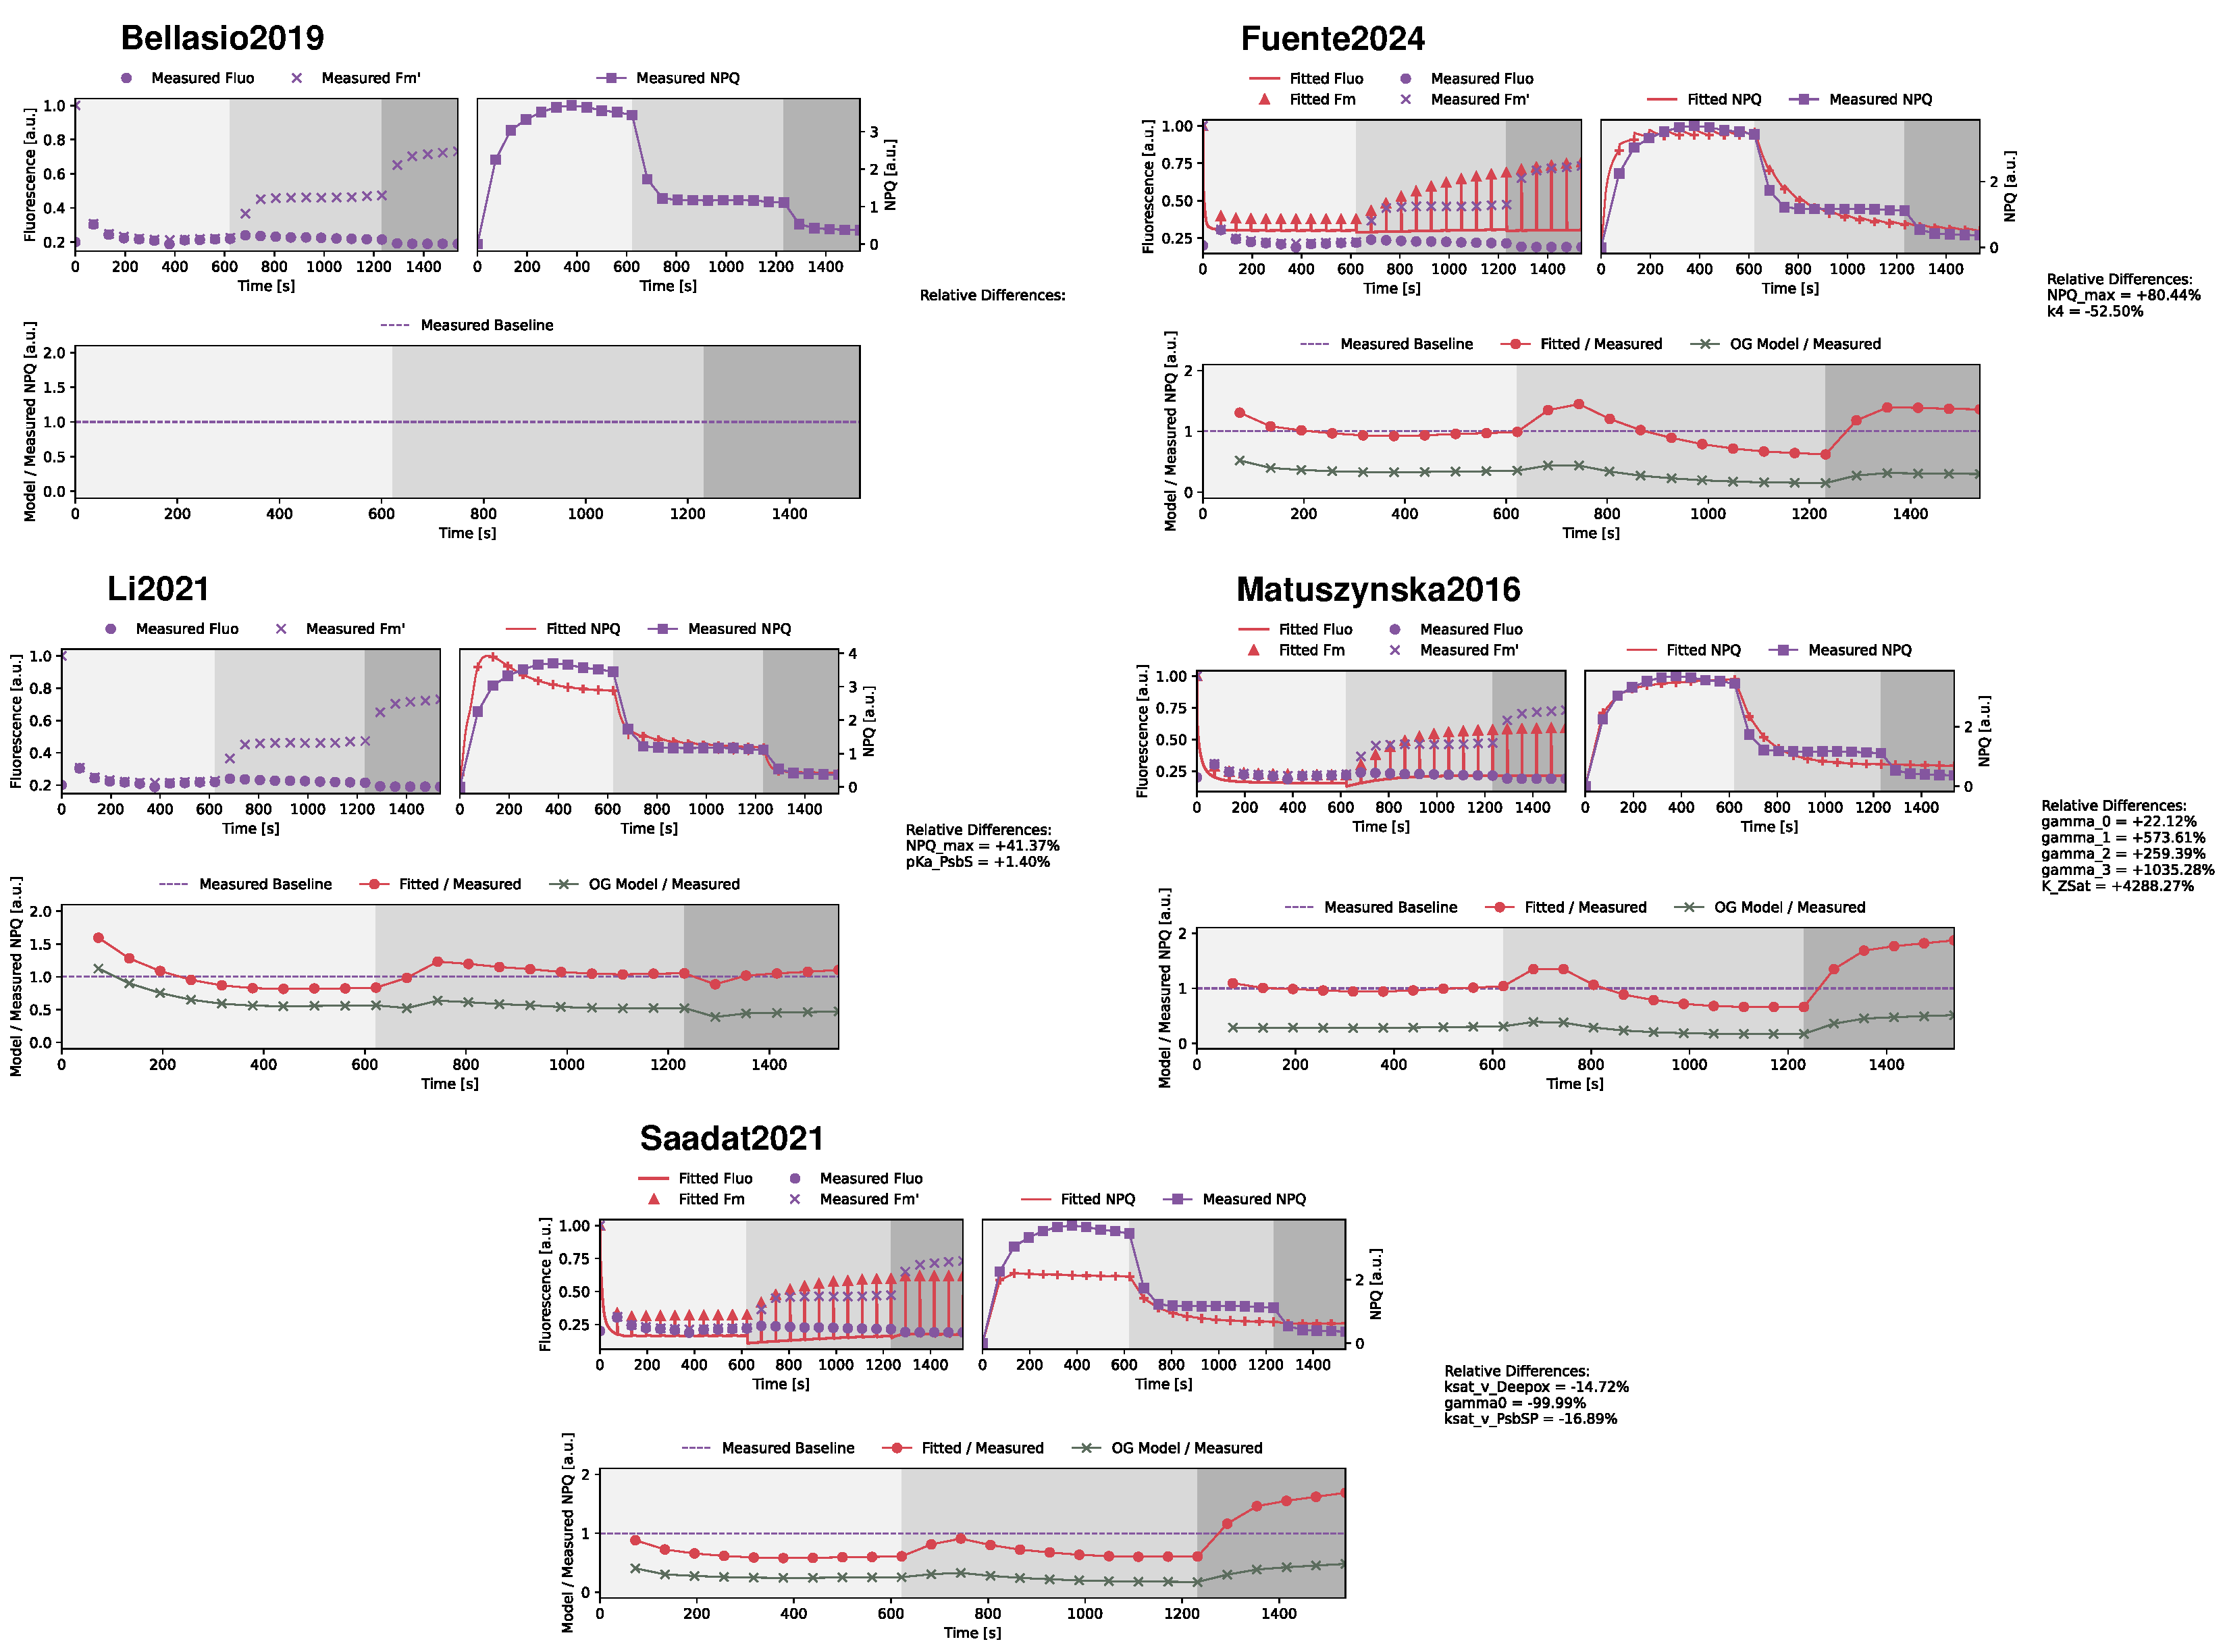
\includegraphics[width=\textwidth]{Figures/Demonstrations/fitting.pdf}
    \captionprof{Combined Fitting of NPQ demonstrations of all models.}{Sample fitting to experimental \glsentryfull{npq} data. The \glsentryshort{npq} data used is taken from experimental work published in von Bismarck (2022)~\cite{vonbismarckLightAcclimationInteracts2023} and was acquired using Maxi Imaging-PAM (Walz, Germany) using Col-0 \glsentryfull{arabidopsis} plants. It is assumed that the experiment follows the default \glsentryshort{pam} protocol of the machine, as no other experimental protocol has been given. Therefore, the protocol of each simulation follows the data given, where the length of one saturating pulse is set to \qty{720}{\micro\second} at a light intensity of \qty{5000}{\micro\mol\per\square\meter\per\second}. The light protocol consists of a dark adaptation period of 30 minutes to acclimate the simulation conditions. Then the actual protocol starts with a longer phase of high actinic light (\qty{903}{\micro\mol\per\square\meter\per\second}) for approximately 10 minutes, followed by a lower actinic light of (\qty{90}{\micro\mol\per\square\meter\per\second}) for 10 minutes, and then 5 minutes of a dark period. During each phase, saturating pulses are given approximately every 60 seconds. As the experimental data also provides exact time points for each pulse, these were taken as reference for the protocol and not the general time intervals. In the experimental work, the dark period consists of actual darkness, whereas in the simulation a low light intensity of \qty{40}{\micro\mol\per\square\meter\per\second} is used to avoid numerical issues. The fitting is performed using the \texttt{lmfit} package in Python with the leastsquare method. On top of that, a standard scaling towards the experimental data is done, to keep the fitting results in the same order of magnitude. To help the fitting converge, weights are applied to the data points, which are defined as the reciprocal of the standard deviation. These settings set are not to be taken as set in stone, as fitting is a highly experimental process and differing settings might be required depending on the model and data used. These settings are a basic starting point for fitting data to a model. The hardest and most impactful decision while fitting is the choice of parameters to fit. There are many ways to find which parameters may be most impactful to fit, such as sensitivity analysis or metabolic control analysis. However, either way experimenting with different parameter sets is always required to find the best fitting practice, which differs for each model and also data to fit to.}
    \label{fig:fit-demon}
\end{figure}

\subsection{Website}

When arriving on the \greensloth{} website, the user is first greeted with the Logo and the motto of the project, "Photosynthesis Models at your Pace"~\figref{fig:website-landingpage}. At the top of the page is a navigation bar, where the user can click to access different pages of the site. These are "Home", "Models", "GreenSloth" with a GitHub logo, "Compare", "How to Use", "About Us", and "Impressum". The "Home" page is the landing page of the website, that continues with an arrow pointing down to find out more. This brings the user to a section that explains the motivation of the project briefly, and then to another section that explains how to use the site. This section is also accessed by the "How To Use" navigation link in the top navigation bar and is separated into the three main aspects that \greensloth{} tries to provide: "Search", "Summary", and "Comparison"~\figref{fig:website-landingpage}. The "Search" part explains how the website's structure allows users to easily find models of photosynthesis, without the need of doing an intensive literature search. The "Summary" part explains how each model was prepared for \greensloth{}, including the detailed presentation of the model, the validation of the model, and the demonstrations performed. The "Compare" part explains how a direct comparison between models is made possible on the website. The user can however go one step further down, to a schematic overview of the photosynthetic machinery, where the user can click on different components that directly brings them to the "Models" page with the clicked machinery as a tag pre-selected.

\begin{figure}
    \centering
    \includegraphics[width=0.7\textwidth]{Figures/Website/landingpage.png}
    \captionprof{Screenshot of the landing page of the \greensloth{} website.}{A screenshot was done of the landing page of the \greensloth{} website, in a full screen mode. The top includes a navigation bar with links to the different pages of the website, and the main section includes the logo and motto of the project.}
    \label{fig:website-landingpage}
\end{figure}

\begin{figure}
    \centering
    \includegraphics[width=0.7\textwidth]{Figures/Website/howtouse.png}
    \captionprof{Screenshot of the How To Use page of the \greensloth{} website.}{A screenshot was done of the How To Use page of the \greensloth{} website, in a full screen mode. The top includes a navigation bar with links to the different pages of the website, and the main section includes three buttons, "Search", "Summary", and "Compare". They all independently show a section of text explaining the respective aspect of the website. These three aspects represent the three main aspect of model searching, understanding, and comparing that \greensloth{} tries to provide.}
    \label{fig:website-howtouse}
\end{figure}

\begin{figure}
    \centering
    \includegraphics[width=0.4\textwidth]{Figures/Website/machienry.png} \hspace{0.1\textwidth} \includegraphics[width=0.4\textwidth]{Figures/Website/machinery-select.png}
    \captionprof{Screenshot of the Machinery page of the \greensloth{} website.}{A screenshot was done of the page showing the photosynthesis machinery of the \greensloth{} website, in a full screen mode. The top includes a navigation bar with links to the different pages of the website, and the main section includes a schematic overview of the photosynthetic machinery, where the user can click on different components that directly brings them to the "Models" page with the clicked machinery as a tag pre-selected. On the left is the full schematic, while on the right is the representation, when the user hovers over one part of the machinery, in this case the "PSII" part. The hovering causes the all other parts to lose their color.}
    \label{fig:website-machienry}
\end{figure}

The "Models" page includes a search bar at the top, where the user can search for models solely by their name. Additionally, next to the bar is a button that opens the tag selection box. This allows the user to list all the models that have a specific tag, which can be related to the photosynthetic machinery, the demonstrations that can be performed with the model, or more~\figref{fig:website-howtouse}. The models are presented row by row, with their name and schemes for the easiest recognition. The user can click on the name of a model and be brought to that model's page.

\begin{figure}
    \centering
    \includegraphics[width=0.7\textwidth]{Figures/Website/modelpage.png}
    \captionprof{Screenshot of the Models page of the \greensloth{} website.}{A screenshot was done of the Models page of the \greensloth{} website, in a full screen mode. The top includes a navigation bar with links to the different pages of the website, and the main section includes a list of models that are available in the database. The list can be filtered by tags that are selected in the tag selection box.}
    \label{fig:website-modelpage}
\end{figure}

After choosing a model, the user is brought onto a page dedicated to that specific model~\figref{fig:website-model-top}. This page includes a sidebar on the left, which enables an easier navigation through the different sections of the page, which are "Summary", "ODE System", "Derived Quantities", "Parameters", "Derived Parameters", "Rates", "Figures", and "Demonstrations". At the top of the page, the name of the model is shown, along with the respective DOI as a link. Below that are two buttons, one to directly bring the user to the GitHub repository of that specific model, with a last update date, and another button that brings the user to the compare page, with this specific model already chosen. Briefly after these buttons, the summary section starts, with the scheme of the model on the left and a brief overview on what the model entails and how the implementation was done on the right. After that section, all the information of the model is shown in a table format, with the respective mathematical equations shown in a \LaTeX format. At the end, the figures and demonstrations sections showcase the recreations of the publication figures and the demonstrations that were performed, with a brief description. Each of the figures and demonstrations are in a collapsable box, to avoid overwhelming the user with too much information at once. If the user whishes to see details compared between the different models, they can click on the "Compare" in the sidebar or the top of the model page, which brings them to the compare page with the model already chosen.

\begin{figure}
    \centering
    \includegraphics[width=0.7\textwidth]{Figures/Website/model-top.png}
    \captionprof{Screenshot of a model page of the \greensloth{} website.}{A screenshot was done of the Fuente2024 model page of the \greensloth{} website, in a full screen mode. The top includes a navigation bar with links to the different pages of the website, and the main section includes a sidebar to navigate that specific page on the left and each section, one after another on the right. These sections are: "Summary", "ODE System", "Derived Quantities", "Parameters", "Derived Parameters", "Rates", "Figures", and "Demonstrations".}
    \label{fig:website-model-top}
\end{figure}

Arrived at the compare page, the user can choose two models from a dropdown menu and compare them side by side in five different categories. The first is the "Variables" category, that shows a Venn diagram of all the variables included in the models~\figref{fig:website-compare-var}. This Venn diagram is supposed to highlight in which variables the models overlap, but due to design and space issues, a figurative diagram is shown in the middle, with the actual variables listed to the left, right, or under it. The variables on the left are unique to the model on the left, and the same goes for the variables on the right, of course to the right sided chosen model. The variables underneath are all the variables, both models have in common. These are clickable, and when clicked, brings the user to the next category, the "Simulation".

\begin{figure}
    \centering
    \includegraphics[width=0.7\textwidth]{Figures/Website/compare-var.png}
    \captionprof{Screenshot of the compare page of the \greensloth{} website, with the variables category selected.}{A screenshot was done of the compare page of the \greensloth{} website, in a full screen mode. The top includes a navigation bar with links to the different pages of the website, and the main section includes two select boxes to choose the models to compare, and five different buttons that represent different categories to compare. The "Variables" category is selected, which shows a Venn diagram of all the variables included in the models. The variables on the left are unique to the model on the left, and the same goes for the variables on the right, of course to the right sided chosen model. The variables underneath are all the variables, both models have in common.}
    \label{fig:website-compare-var}
\end{figure}

In this category, the user can choose an overlapping variable between both models, and see a simple simulation over time~\figref{fig:website-compare-sim}. The protocol used always starts with a period of \qty{50}{\micro\mol\per\square\meter\per\second} light intensity for 10 seconds, followed by \qty{50}{\second} of light. This category also includes a slider, that lets the user change the light intensity of the light phase, giving a dynamic and instant way to showcase a simple simulation of the models. It has to be noted, that these simulations are not done live on the website, but have been pre-simulated for each of the models, and only the results are shown on the website. If the user, whishes to get more information on the models themselves, they can click on the "Information" tab, which brings them to a side by side numeric table view of all the meta-information of the models, such as the number of variables, parameters, and more.

\begin{figure}
    \centering
    \includegraphics[width=0.7\textwidth]{Figures/Website/compare-sim.png}
    \captionprof{Screenshot of the compare page of the \greensloth{} website, with the simulation category selected.}{A screenshot was done of the compare page of the \greensloth{} website, in a full screen mode. The top includes a navigation bar with links to the different pages of the website, and the main section includes two select boxes to choose the models to compare, and five different buttons that represent different categories to compare. The "Simulation" category is selected, which shows a simple simulation over time of an overlapping variable between both models. Here, the results of \glsentryfull{pq_ox} from the simulation of the Saadat2021 and the Fuente2024 at a \glsentryfull{ppfd} of \qty{100}{\micro\mol\per\square\meter\per\second} are shown.}
    \label{fig:website-compare-sim}
\end{figure}

The penultimate category is that of the "Demonstrations", where the user is able to choose from the demonstrations performed on the models, and see the results side by side~\figref{fig:website-compare-demon}. From the representing figure at the top, to the brief description underneath it. Then, the last category, "Schemes", is where both models' schemes are shown side by side, to easily compare the structure of the models~\figref{fig:website-compare-schemes}.

\begin{figure}
    \centering
    \includegraphics[width=0.7\textwidth]{Figures/Website/compare-demon.png}
    \captionprof{Screenshot of the compare page of the \greensloth{} website, with the demonstrations category selected.}{A screenshot was done of the compare page of the \greensloth{} website, in a full screen mode. The top includes a navigation bar with links to the different pages of the website, and the main section includes two select boxes to choose the models to compare, and five different buttons that represent different categories to compare. The "Demonstrations" category is selected, which shows two other select boxes, which contain the five possible demonstrations that were performed on each model. The Li2021 model on the left shows the PAM simulation, while the Matuszynska2016 model on the right shows the Day Simulation. The respective figures of the demonstrations are shown at the top, with a brief description of the demonstration underneath.}
    \label{fig:website-compare-demon}
\end{figure}

\begin{figure}
    \centering
    \includegraphics[width=0.7\textwidth]{Figures/Website/compare-schemes.png}
    \captionprof{Screenshot of the compare page of the \greensloth{} website, with the schemes category selected.}{A screenshot was done of the compare page of the \greensloth{} website, in a full screen mode. The top includes a navigation bar with links to the different pages of the website, and the main section includes two select boxes to choose the models to compare, and five different buttons that represent different categories to compare. The "Schemes" category is selected, which shows both models' schemes side by side. On the left, the Fuente2024 model is shown, while on the right, the Li2021 model is shown.}
    \label{fig:website-compare-schemes}
\end{figure}

The last two pages, "About Us" and "Impressum", include either information about the project and the team behind it, or legal information about the project. This, wraps up the entire \greensloth{} Website, and can be found here: \url{https://greensloth.rwth-aachen.de/}.